\documentclass[12pt,]{article}
%\usepackage{lmodern}  Melissa removed to deal with font rendering issue
\usepackage{amssymb,amsmath}
\usepackage{ifxetex,ifluatex}
\usepackage{fixltx2e} % provides \textsubscript

%Melissa removed the following section to deal with font rendering issue
%\ifnum 0\ifxetex 1\fi\ifluatex 1\fi=0 % if pdftex
%  \usepackage[T1]{fontenc}
%  \usepackage[utf8]{inputenc}
%%\else % if luatex or xelatex
%  \ifxetex
%    \usepackage{mathspec}
%  \else
%    \usepackage{fontspec}
%  \fi
%  \defaultfontfeatures{Ligatures=TeX,Scale=MatchLowercase}
%  \newcommand{\euro}{€}
%%%%%%\fi

% use upquote if available, for straight quotes in verbatim environments
\IfFileExists{upquote.sty}{\usepackage{upquote}}{}
% use microtype if available
\IfFileExists{microtype.sty}{%
\usepackage{microtype}
\UseMicrotypeSet[protrusion]{basicmath} % disable protrusion for tt fonts
}{}
\usepackage[margin=1in]{geometry}
\usepackage{hyperref}
\PassOptionsToPackage{usenames,dvipsnames}{color} % color is loaded by hyperref
\hypersetup{unicode=true,
            pdftitle={Status of Big Skate (Beringraja binoculata) Off the U.S. Pacific Coast in 2019},
            pdfborder={0 0 0},
            breaklinks=true}
\urlstyle{same}  % don't use monospace font for urls
\usepackage{graphicx,grffile}
\makeatletter
\def\maxwidth{\ifdim\Gin@nat@width>\linewidth\linewidth\else\Gin@nat@width\fi}
\def\maxheight{\ifdim\Gin@nat@height>\textheight\textheight\else\Gin@nat@height\fi}
\makeatother
% Scale images if necessary, so that they will not overflow the page
% margins by default, and it is still possible to overwrite the defaults
% using explicit options in \includegraphics[width, height, ...]{}
\setkeys{Gin}{width=\maxwidth,height=\maxheight,keepaspectratio}
\setlength{\parindent}{0pt}
\setlength{\parskip}{6pt plus 2pt minus 1pt}
\setlength{\emergencystretch}{3em}  % prevent overfull lines
\providecommand{\tightlist}{%
  \setlength{\itemsep}{0pt}\setlength{\parskip}{0pt}}
\setcounter{secnumdepth}{5}

%%% Use protect on footnotes to avoid problems with footnotes in titles
\let\rmarkdownfootnote\footnote%
\def\footnote{\protect\rmarkdownfootnote}

%%% Change title format to be more compact
\usepackage{titling}

% Create subtitle command for use in maketitle
\newcommand{\subtitle}[1]{
  \posttitle{
    \begin{center}\large#1\end{center}
    }
}

\setlength{\droptitle}{-2em}
  \title{Status of Big Skate (\emph{Beringraja binoculata}) Off the U.S. Pacific
Coast in 2019}
  \pretitle{\vspace{\droptitle}\centering\huge}
  \posttitle{\par}
  \author{}
  \preauthor{}\postauthor{}
  \date{}
  \predate{}\postdate{}


% This file contains all of the LaTeX packages you may need to compile the document
% Documentation for each package can be found onlines
\usepackage{tabularx}                                             % table environment providing flexibility
\usepackage{caption}                                              % for creating captions  
\usepackage{longtable}                                            % allows tables to span multiple pages
\usepackage{rotating}                                             % allows for sideways tables
\usepackage{float}                                                % floating environments; may not need in rmarkdown
\usepackage{placeins}                                             % keeps floats from moving
\usepackage{indentfirst}                                          % indents first paragraph of a section
\usepackage{mdwtab}                                               % continued float multi-page figure
\usepackage{enumerate}                                            % create lists
\usepackage{hyperref}                                             % highlight cross references
\hypersetup{colorlinks=true, urlcolor=blue, linktoc=page, linkcolor=blue, citecolor=blue} %define referencing colors
%\usepackage{makebox}                                             % make boxes around text
\usepackage[usenames,dvipsnames]{xcolor}                          % color name options
%\usepackage[space]{grffile}                                      % spaces in file name path
\usepackage{soul}                                                 % highlight text
\usepackage{enumitem}                                             % numbered lists
\usepackage{lineno}                                               % Line numbers; comment out for final
\usepackage{upquote}                                              % produce grave accent in latex
\usepackage{verbatim}                                             % produces verbatim results
\usepackage{fancyvrb}                                             % verbatim in a box
%\usepackage{draftwatermark}                                      % places Draft watermark in background; comment out for final
\usepackage{textcomp}                                             % fixes error with packages interfering
\usepackage{lscape}                                               % rotate pages - to allow for landscape longtables
%\pdfinterwordspaceon                                             % fix loss of inter word spacing
\usepackage{cmap}                                                 % fix mapping characters to unicode
\RequirePackage[linewidth = 1]{pdfcomment}                        % pdf comments
\RequirePackage[l2tabu, orthodox]{nag}                            % checks packages related to the accessibility?
\usepackage[inline]{showlabels}                                   % show table and figure labels; comment out for final
%\RequirePackage[tagged]{accessibilityMeta}


\linenumbers                                                      % specify use of line numbers


\definecolor{light-gray}{gray}{.85}                               % define light-gray as a color
%\usepackage[tagged]{accessibility-meta}

 
%\showlabels[\color{mred}]{label}

% Redefines (sub)paragraphs to behave more like sections
\ifx\paragraph\undefined\else
\let\oldparagraph\paragraph
\renewcommand{\paragraph}[1]{\oldparagraph{#1}\mbox{}}
\fi
\ifx\subparagraph\undefined\else
\let\oldsubparagraph\subparagraph
\renewcommand{\subparagraph}[1]{\oldsubparagraph{#1}\mbox{}}
\fi

\begin{document}
\maketitle


\begin{center}
\thispagestyle{empty}

\vspace{.7cm}

% 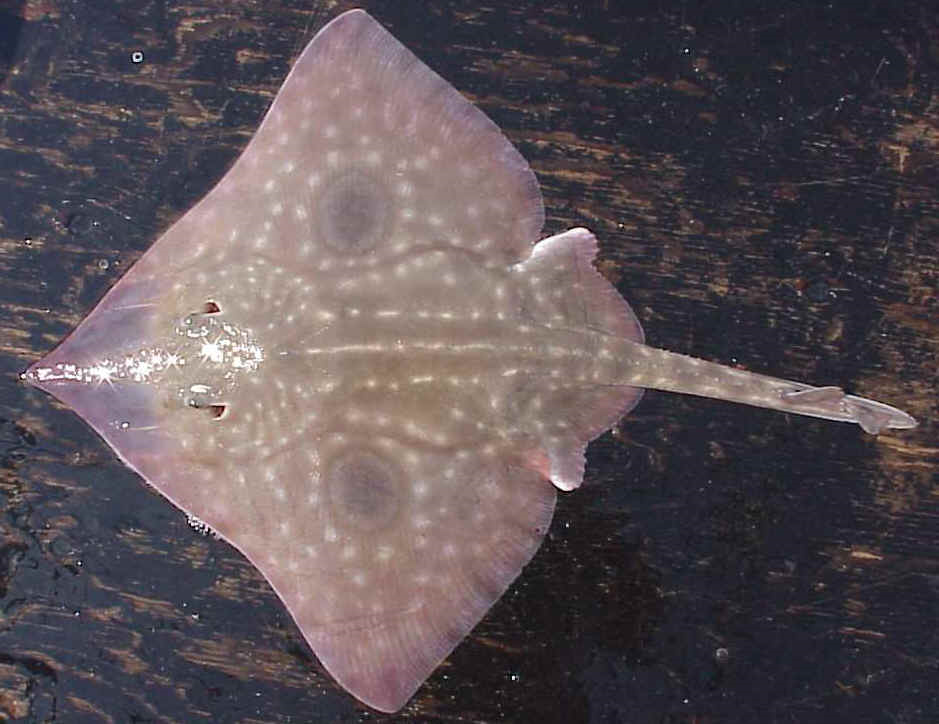
\includegraphics{cover_photo}~\\[1cm]
\pdftooltip{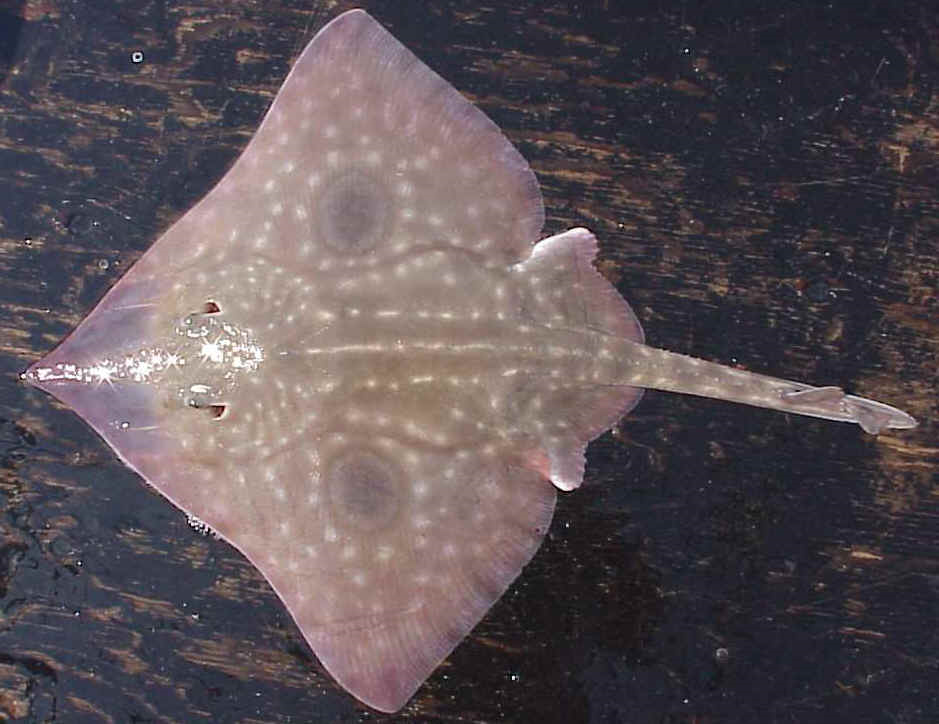
\includegraphics{cover_photo}}{This is a fish.}

\vspace{.5cm}

Ian G. Taylor\textsuperscript{1}\\
Vladlena Gertseva\textsuperscript{1}\\
Joseph Bizzarro\textsuperscript{2}\\
Andi Stephens\textsuperscript{3}\\

\vspace{.7cm}

\small

\textsuperscript{1}Northwest Fisheries Science Center, U.S. Department of Commerce, National Oceanic and Atmospheric Administration, National Marine Fisheries Service, 2725 Montlake Boulevard East, Seattle, Washington 98112\\

\vspace{.3cm}

\textsuperscript{2}Southwest Fisheries Science Center, U.S. Department of Commerce, National Oceanic and Atmospheric Administration, National Marine Fisheries Service, 110 Shaffer Road, Santa Cruz, California 95060\\

\vspace{.3cm}

\textsuperscript{3}Northwest Fisheries Science Center, U.S. Department of Commerce, National Oceanic and Atmospheric Administration, National Marine Fisheries Service, 2032 S.E. OSU Drive Newport, Oregon 97365


\vspace{.5cm}

\vfill
DRAFT SAFE\\
Disclaimer: This information is distributed solely for the purpose of pre-dissemination
peer review under applicable information quality guidelines. It has not been formally
disseminated by NOAA Fisheries. It does not represent and should not be construed to
represent any agency determination or policy. 

\vspace{.3cm}
%Bottom of the page
%{\large \today}


\newpage{\thispagestyle{empty}}


\begin{flushleft}
This report may be cited as:

Taylor, I.G., Gertseva, V., Bizzarro, J., and Stephens, A. Status of Big Skate (\emph{Beringraja binoculata}) Off the U.S. West Coast, 2019. Pacific Fishery Management Council, Portland, OR. Available from http://www.pcouncil.org/groundfish/stock-assessments/
\end{flushleft}

\maketitle

\pagenumbering{roman}
\setcounter{page}{1}
\end{center}

{
\setcounter{tocdepth}{4}
\tableofcontents
}
\setlength{\parskip}{5mm plus1mm minus1mm}
\pagebreak

\pagenumbering{arabic}

\renewcommand{\thefigure}{\alph{figure}}
\renewcommand{\thetable}{\alph{table}}

\hypertarget{executive-summary}{%
\section*{Executive Summary}\label{executive-summary}}
\addcontentsline{toc}{section}{Executive Summary}

\hypertarget{stock}{%
\subsection*{Stock}\label{stock}}
\addcontentsline{toc}{subsection}{Stock}

This assessment reports the status of the Big Skate
(\emph{Beringraja binoculata}) resource in U.S. waters off the coast of
\ldots{} using data through 2018.

\hypertarget{catches}{%
\subsection*{Catches}\label{catches}}
\addcontentsline{toc}{subsection}{Catches}

Information on historical landings of Big Skate are available back to
xxxx\ldots{} (Table \ref{tab:Exec_catch}). Commercial landings were
small during the years of World War II, ranging between 329 to 395
metric tons (mt) per year.

(Figures \ref{fig:Exec_catch1}-\ref{fig:Exec_catch2})\\
(Figure \ref{fig:r4ss_catches})

Since 2000, annual total landings of Big Skate have ranged between
135-412 mt, with landings in 2018 totaling 173 mt.

\FloatBarrier

\begin{figure}
\centering
\includegraphics{00_Assessment_Compile_files/figure-latex/unnamed-chunk-15-1.pdf}
\caption{Big Skate catch history for the recreational fleets.
\label{fig:Exec_catch1}}
\end{figure}

\begin{figure}
\centering
\includegraphics{00_Assessment_Compile_files/figure-latex/unnamed-chunk-16-1.pdf}
\caption{Stacked line plot of Big Skate catch history for the commercial
fleets. \label{fig:Exec_catch2}}
\end{figure}

\FloatBarrier

\begin{figure}
\centering
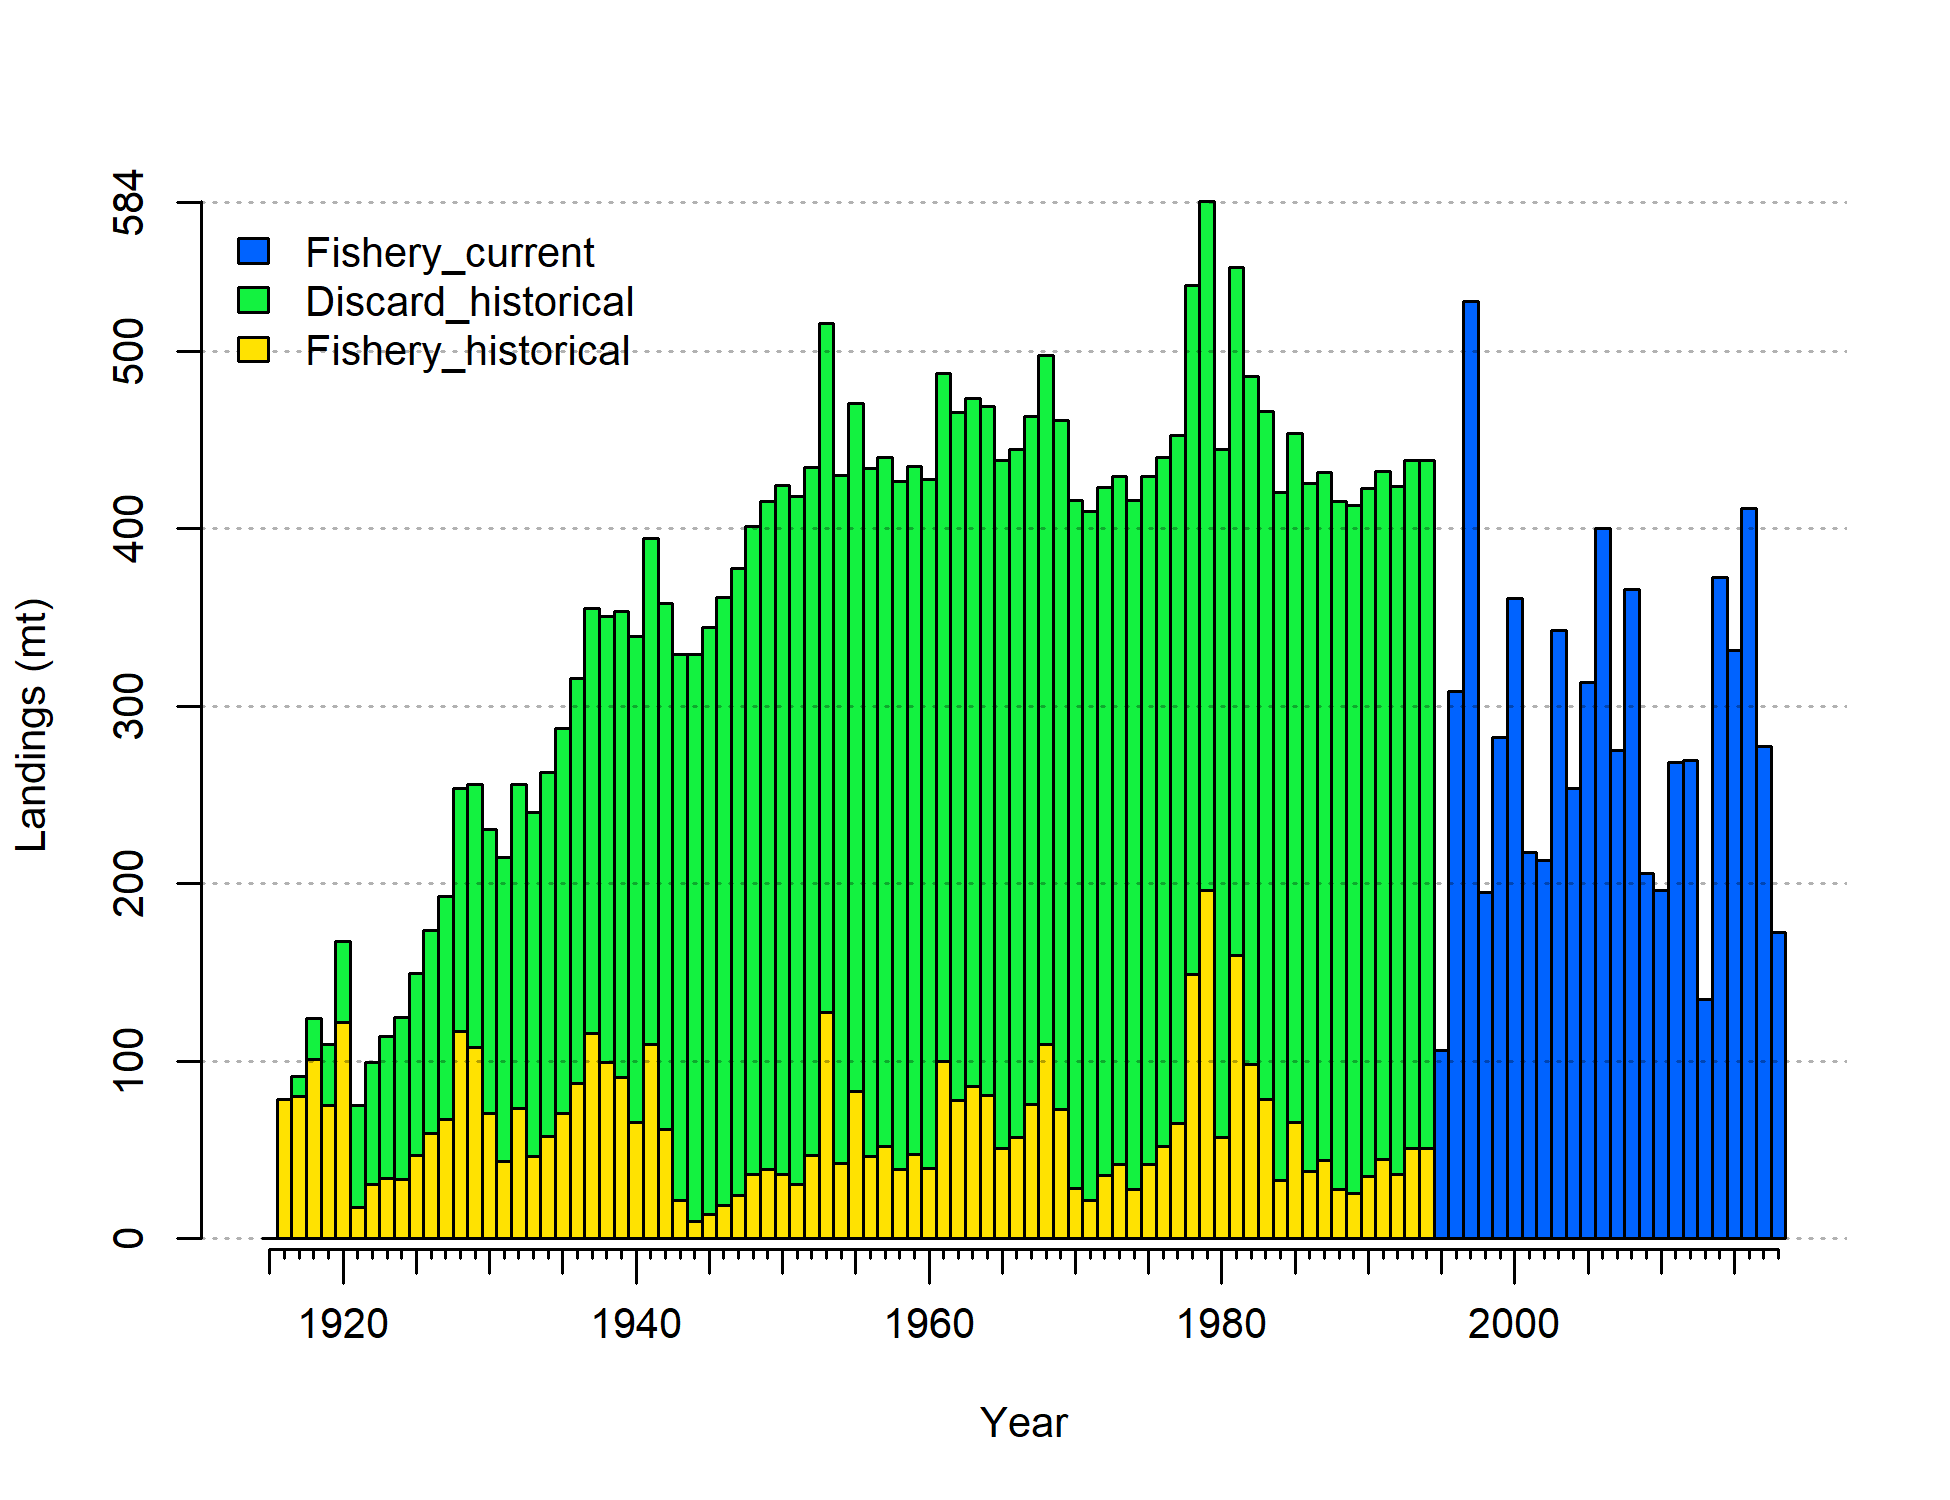
\includegraphics{r4ss/plots_mod1/catch2 landings stacked.png}
\caption{Catch history of Big Skate in the model.
\label{fig:r4ss_catches}}
\end{figure}

\begin{table}[ht]
\centering
\caption{Recent Big Skate landings (mt) by 
                                            fleet.} 
\label{tab:Exec_catch}
\begin{tabular}{l>{\centering}p{1in}>{\centering}p{1in}>{\centering}p{1in}>{\centering}p{.9in}>{\centering}p{.9in}>{\centering}p{.6in}}
  \hline
Year & Landings 1 & Landings 2 & Landings 3 & Landings 4 & Landings 5 & Total \\ 
  \hline
2005 & - & - & - & - & - & - \\ 
  2006 & - & - & - & - & - & - \\ 
  2007 & - & - & - & - & - & - \\ 
  2008 & - & - & - & - & - & - \\ 
  2009 & - & - & - & - & - & - \\ 
  2010 & - & - & - & - & - & - \\ 
  2011 & - & - & - & - & - & - \\ 
  2012 & - & - & - & - & - & - \\ 
  2013 & - & - & - & - & - & - \\ 
  2014 & - & - & - & - & - & - \\ 
   \hline
\end{tabular}
\end{table}

\FloatBarrier

\newpage

\hypertarget{data-and-assessment}{%
\subsection*{Data and Assessment}\label{data-and-assessment}}
\addcontentsline{toc}{subsection}{Data and Assessment}

This the first full assessment for Big Skate, which was last assessed as
part of the ``Other species'' Complex. This assessment uses the newest
version of Stock Synthesis (3.30.xx). The model begins in 1916, and
assumes the stock was at an unfished equilibrium that year.

(Figure \ref{fig:assess_region_map}).

\begin{figure}
\centering
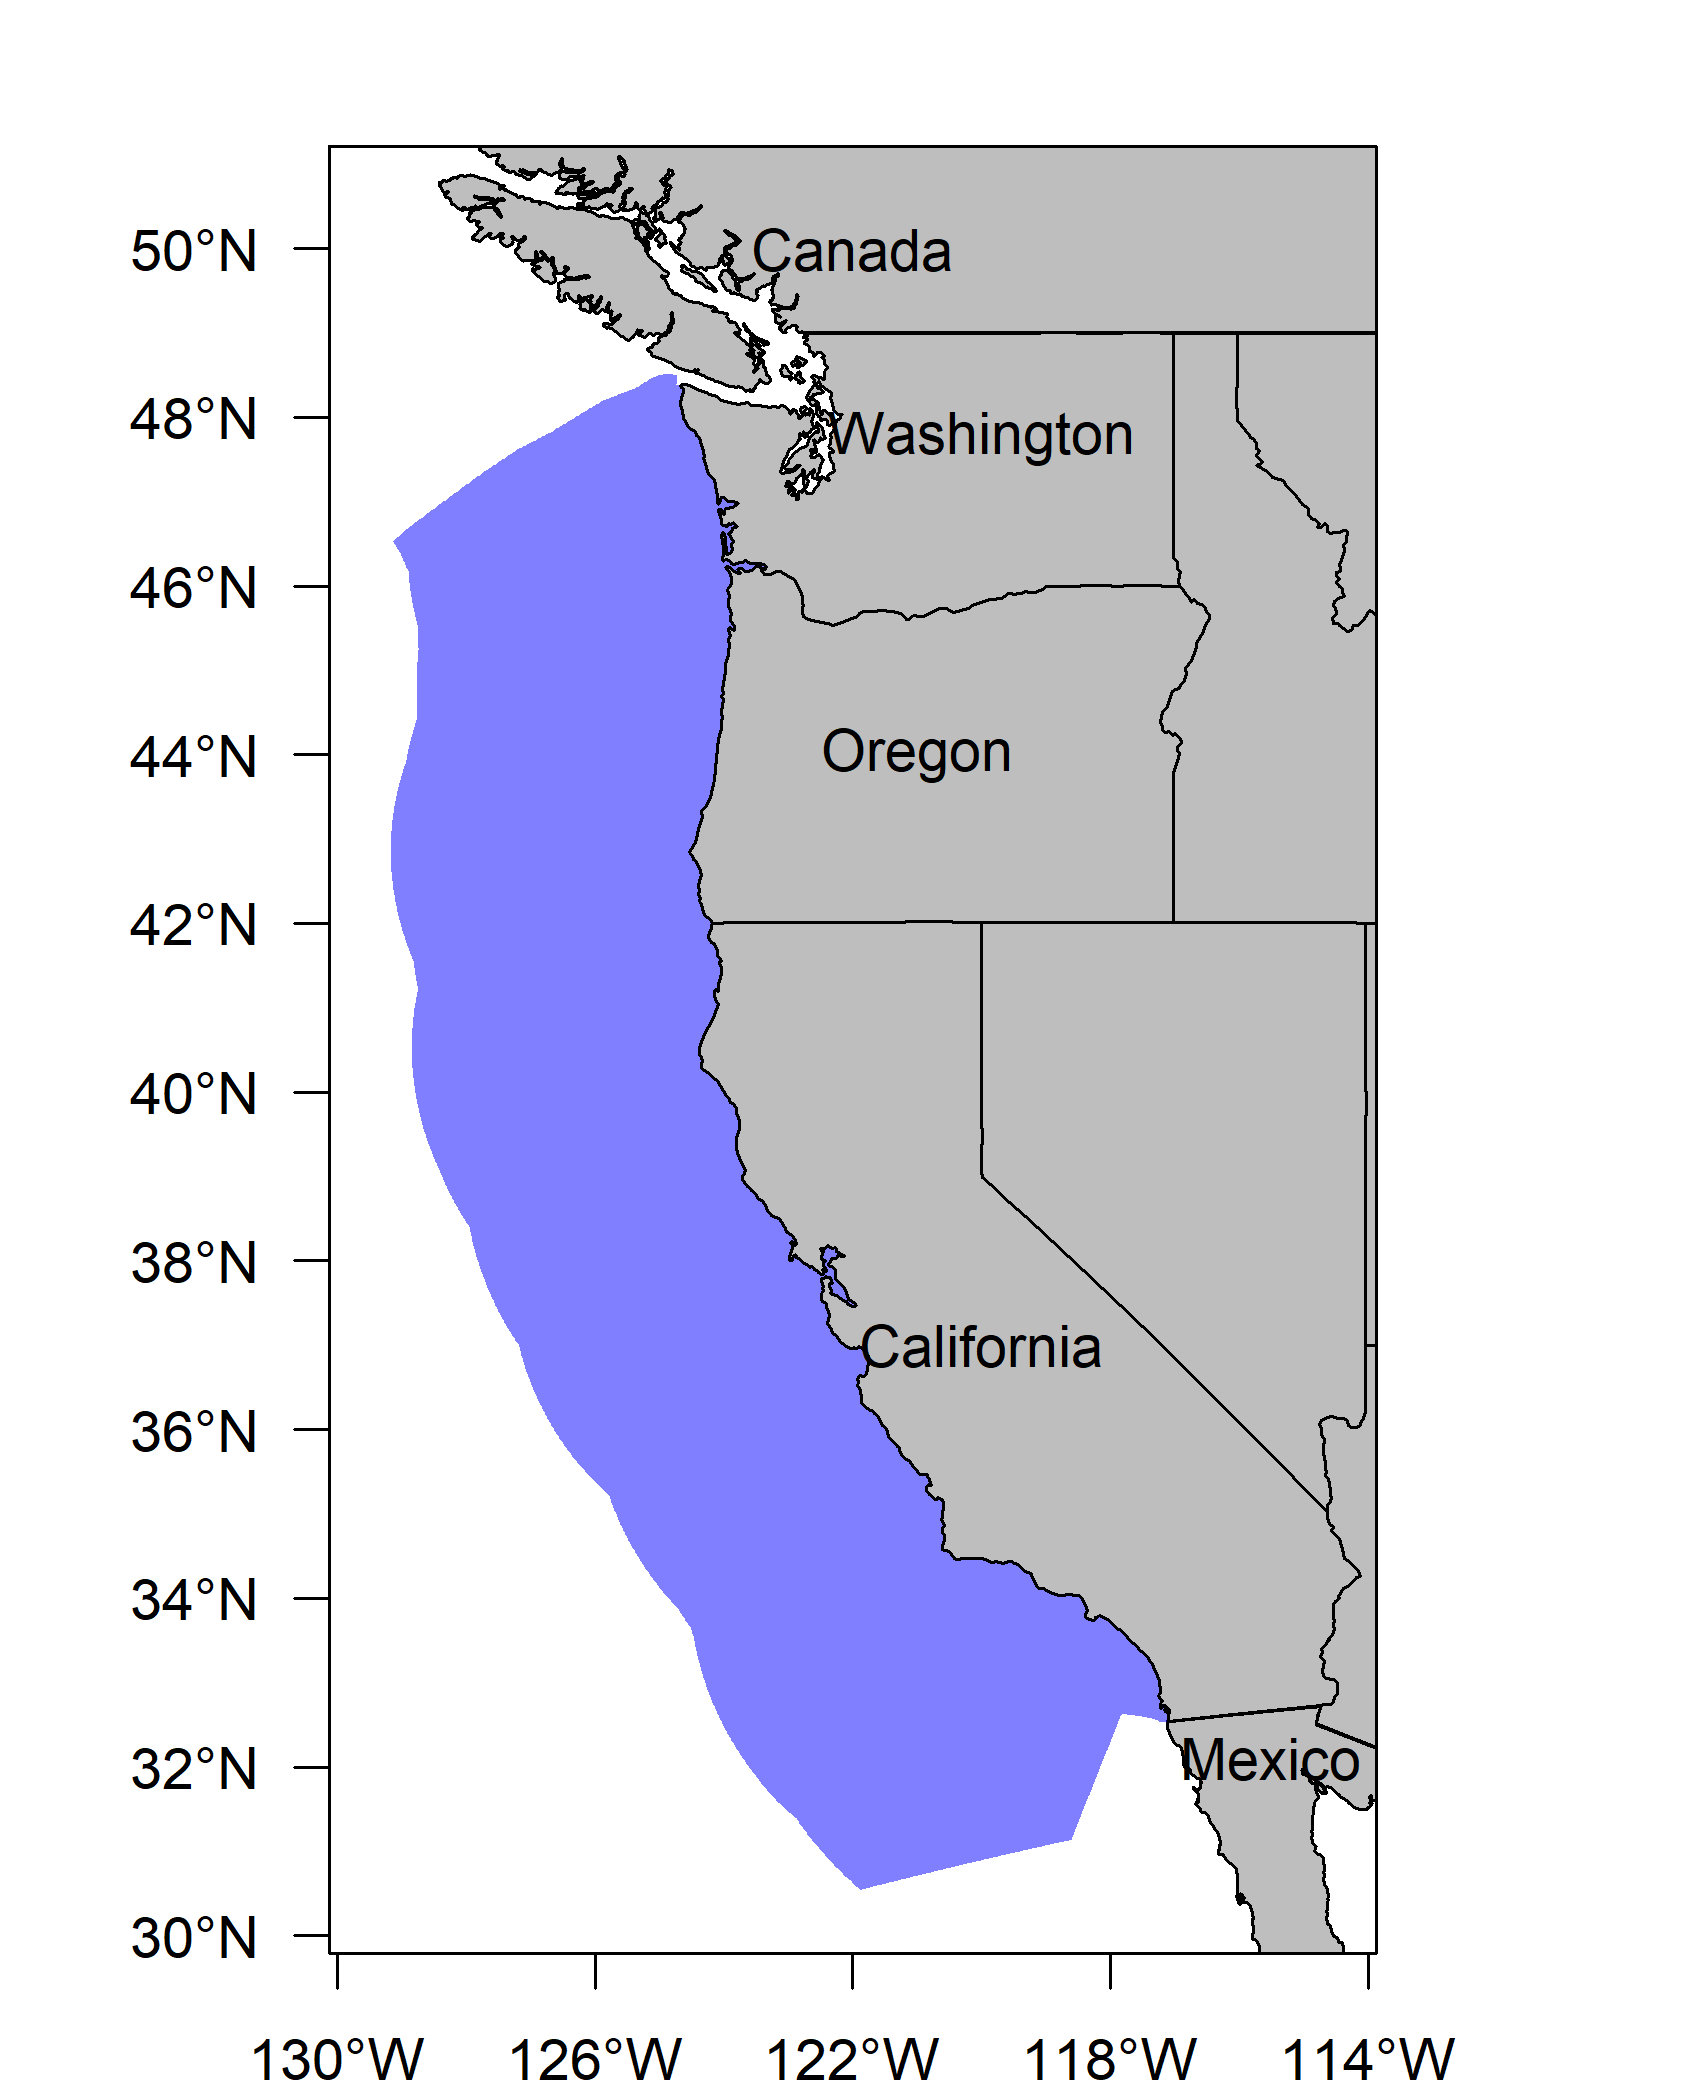
\includegraphics{Figures/assess_region_map.png}
\caption{Map depicting the distribution of California scorpionfish out
to 600 ft. The stock assessment is bounded at Pt. Conception in the
north to the U.S./Mexico border in the south.
\label{fig:assess_region_map}}
\end{figure}

\FloatBarrier

\#\#Stock Biomass\{-\} (Figure \ref{fig:Spawnbio_all} and Table
\ref{tab:SpawningDeplete_mod1}).

The 2018 estimated spawning biomass relative to unfished equilibrium
spawning biomass is above the target of 40\% of unfished spawning
biomass at 99.8\% (95\% asymptotic interval: \(\pm\) 99.8\%-99.8\%)
(Figure \ref{fig:RelDeplete_all}). Approximate confidence intervals
based on the asymptotic variance estimates show that the uncertainty in
the estimated spawning biomass is high.

\FloatBarrier

\begin{table}[ht]
\centering
\caption{Recent trend in beginning of the 
                                      year spawning output and depletion for
                                      the model for Big Skate.} 
\label{tab:SpawningDeplete_mod1}
\begin{tabular}{l>{\centering}p{1.3in}>{\centering}p{1.2in}>{\centering}p{1in}>{\centering}p{1.2in}}
  \hline
Year & Spawning Output (million eggs) & \~{} 95\% confidence interval & Estimated depletion & \~{} 95\% confidence interval \\ 
  \hline
2010 & 70693.200 & (70693.2-70693.2) & 0.998 & (0.998-0.998) \\ 
  2011 & 70697.500 & (70697.5-70697.5) & 0.998 & (0.998-0.998) \\ 
  2012 & 70699.900 & (70699.9-70699.9) & 0.998 & (0.998-0.998) \\ 
  2013 & 70702.400 & (70702.4-70702.4) & 0.998 & (0.998-0.998) \\ 
  2014 & 70709.200 & (70709.2-70709.2) & 0.998 & (0.998-0.998) \\ 
  2015 & 70708.700 & (70708.7-70708.7) & 0.998 & (0.998-0.998) \\ 
  2016 & 70708.900 & (70708.9-70708.9) & 0.998 & (0.998-0.998) \\ 
  2017 & 70706.000 & (70706-70706) & 0.998 & (0.998-0.998) \\ 
  2018 & 70706.500 & (70706.5-70706.5) & 0.998 & (0.998-0.998) \\ 
  2019 & 70709.900 & (70709.9-70709.9) & 0.998 & (0.998-0.998) \\ 
   \hline
\end{tabular}
\end{table}

\FloatBarrier

\begin{figure}
\centering
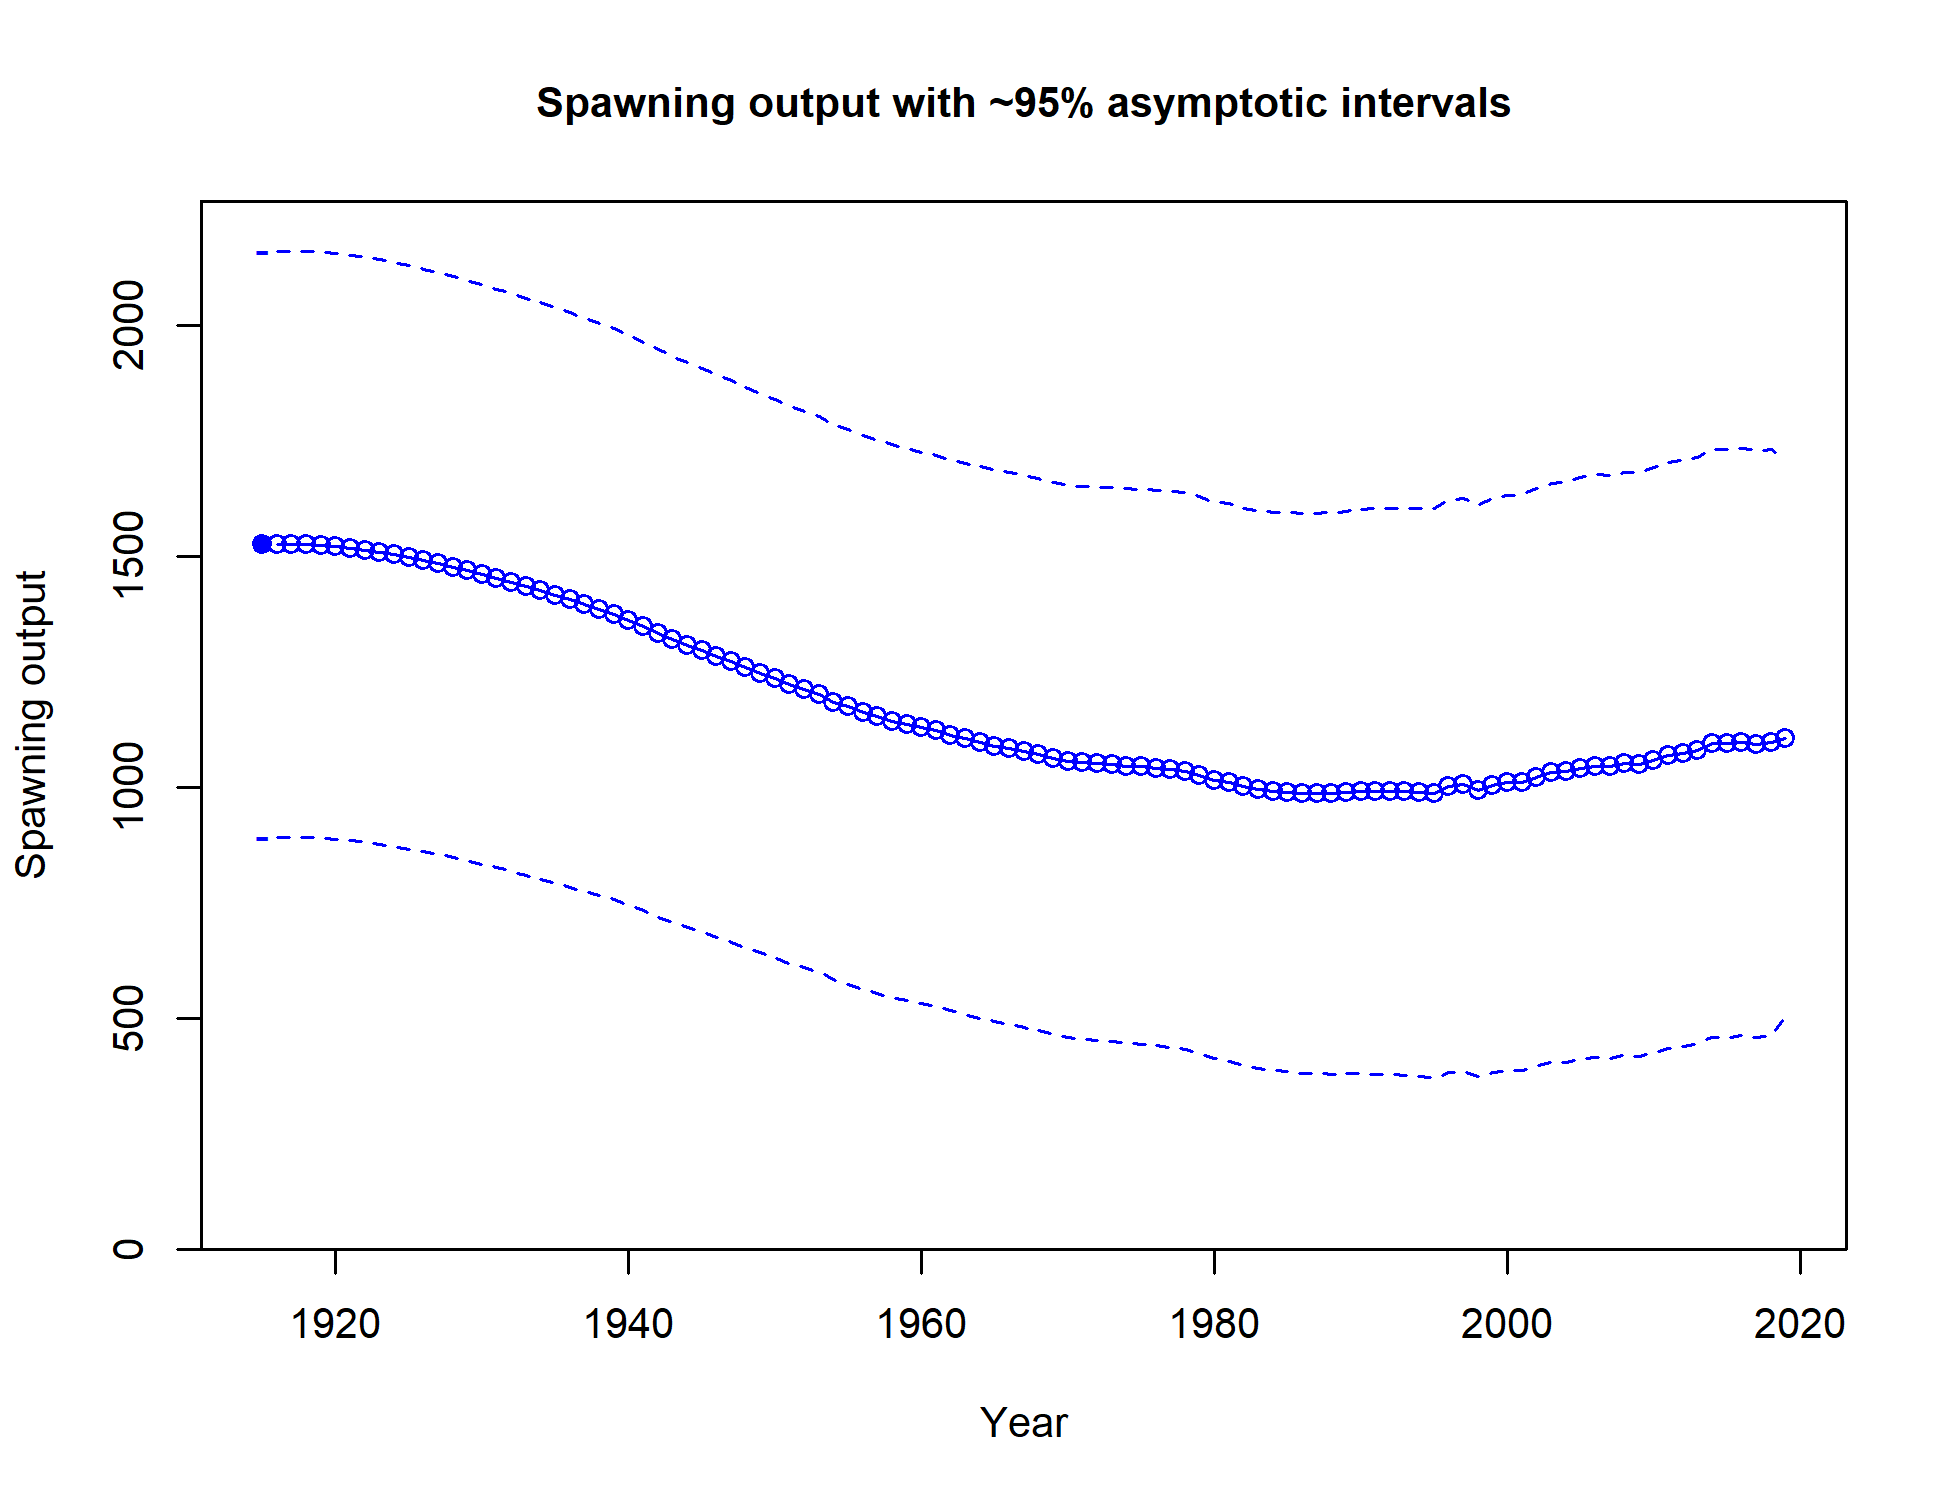
\includegraphics{r4ss/plots_mod1/ts7_Spawning_output_with_95_asymptotic_intervals_intervals.png}
\caption{Time series of spawning biomass trajectory (circles and line:
median; light broken lines: 95\% credibility intervals) for the base
case assessment model. \label{fig:Spawnbio_all}}
\end{figure}

\begin{figure}
\centering
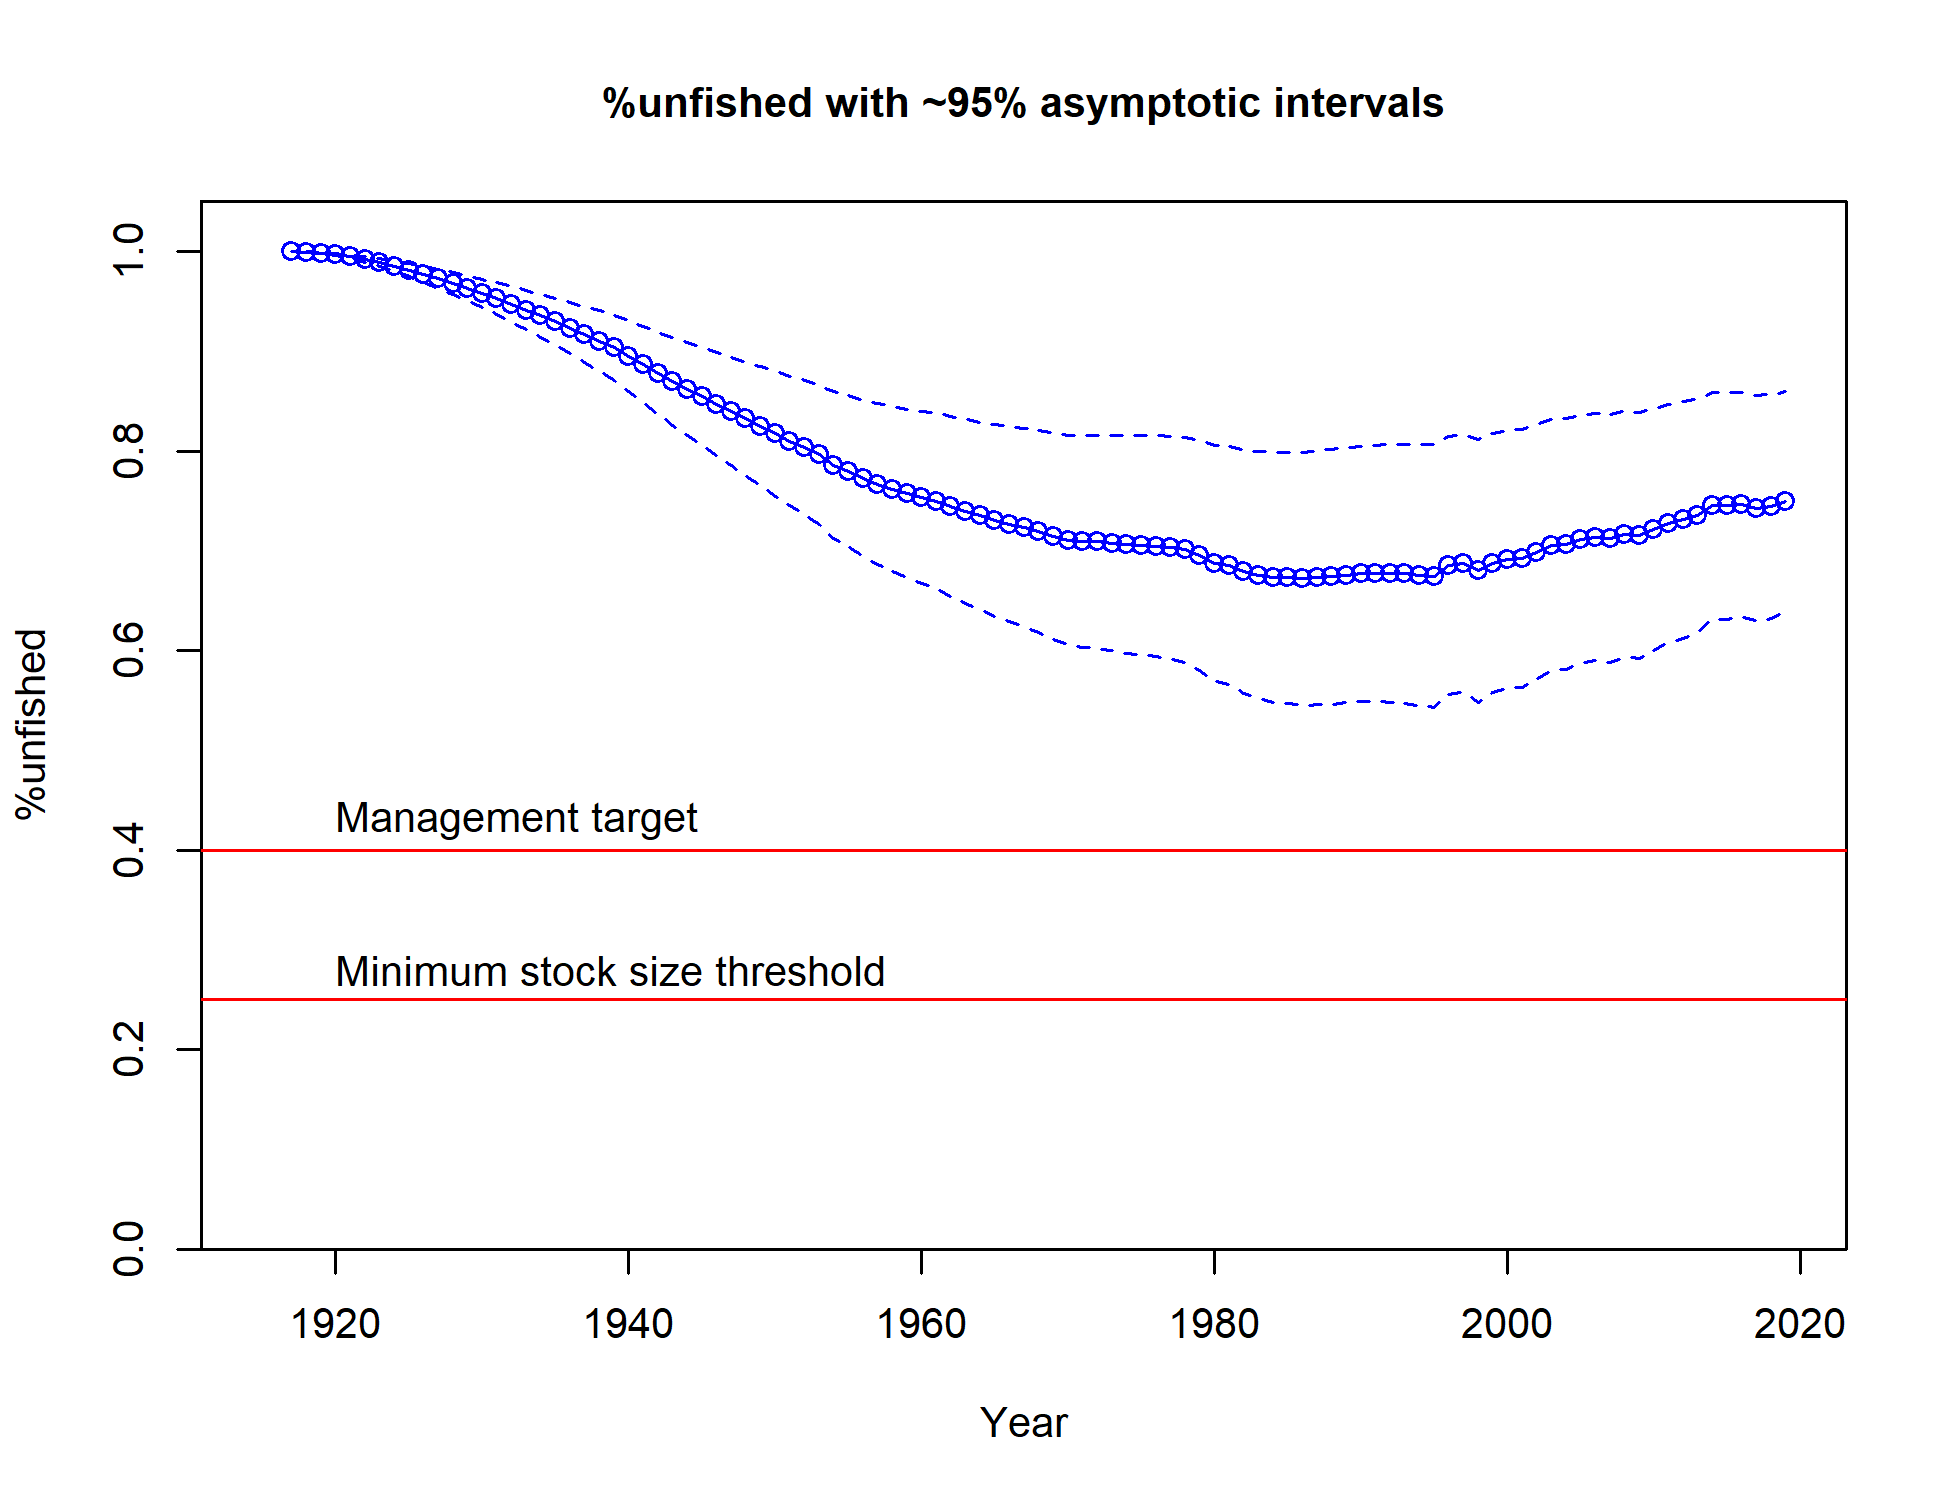
\includegraphics{r4ss/plots_mod1/ts9_Spawning_depletion_with_95_asymptotic_intervals_intervals.png}
\caption{Estimated relative depletion with approximate 95\% asymptotic
confidence intervals (dashed lines) for the base case assessment model.
\label{fig:RelDeplete_all}}
\end{figure}

\FloatBarrier

\hypertarget{recruitment}{%
\subsection*{Recruitment}\label{recruitment}}
\addcontentsline{toc}{subsection}{Recruitment}

Recruitment deviations were estimated from xxxx-xxxx (Figure
\ref{fig:Recruits_all} and Table \ref{tab:Recruit_mod1}).

\begin{table}[ht]
\centering
\caption{Recent recruitment for the model.} 
\label{tab:Recruit_mod1}
\begin{tabular}{>{\centering}p{.8in}>{\centering}p{1.6in}>{\centering}p{1.3in}}
  \hline
Year & Estimated Recruitment (millions) & \~{} 95\% confidence interval \\ 
  \hline
2010 & 749.57 & (749.57 - 749.57) \\ 
  2011 & 749.59 & (749.59 - 749.59) \\ 
  2012 & 749.60 & (749.6 - 749.6) \\ 
  2013 & 749.61 & (749.61 - 749.61) \\ 
  2014 & 749.64 & (749.64 - 749.64) \\ 
  2015 & 749.63 & (749.63 - 749.63) \\ 
  2016 & 749.63 & (749.63 - 749.63) \\ 
  2017 & 749.62 & (749.62 - 749.62) \\ 
  2018 & 749.62 & (749.63 - 749.63) \\ 
  2019 & 749.64 & (749.64 - 749.64) \\ 
   \hline
\end{tabular}
\end{table}

\FloatBarrier

\begin{figure}
\centering
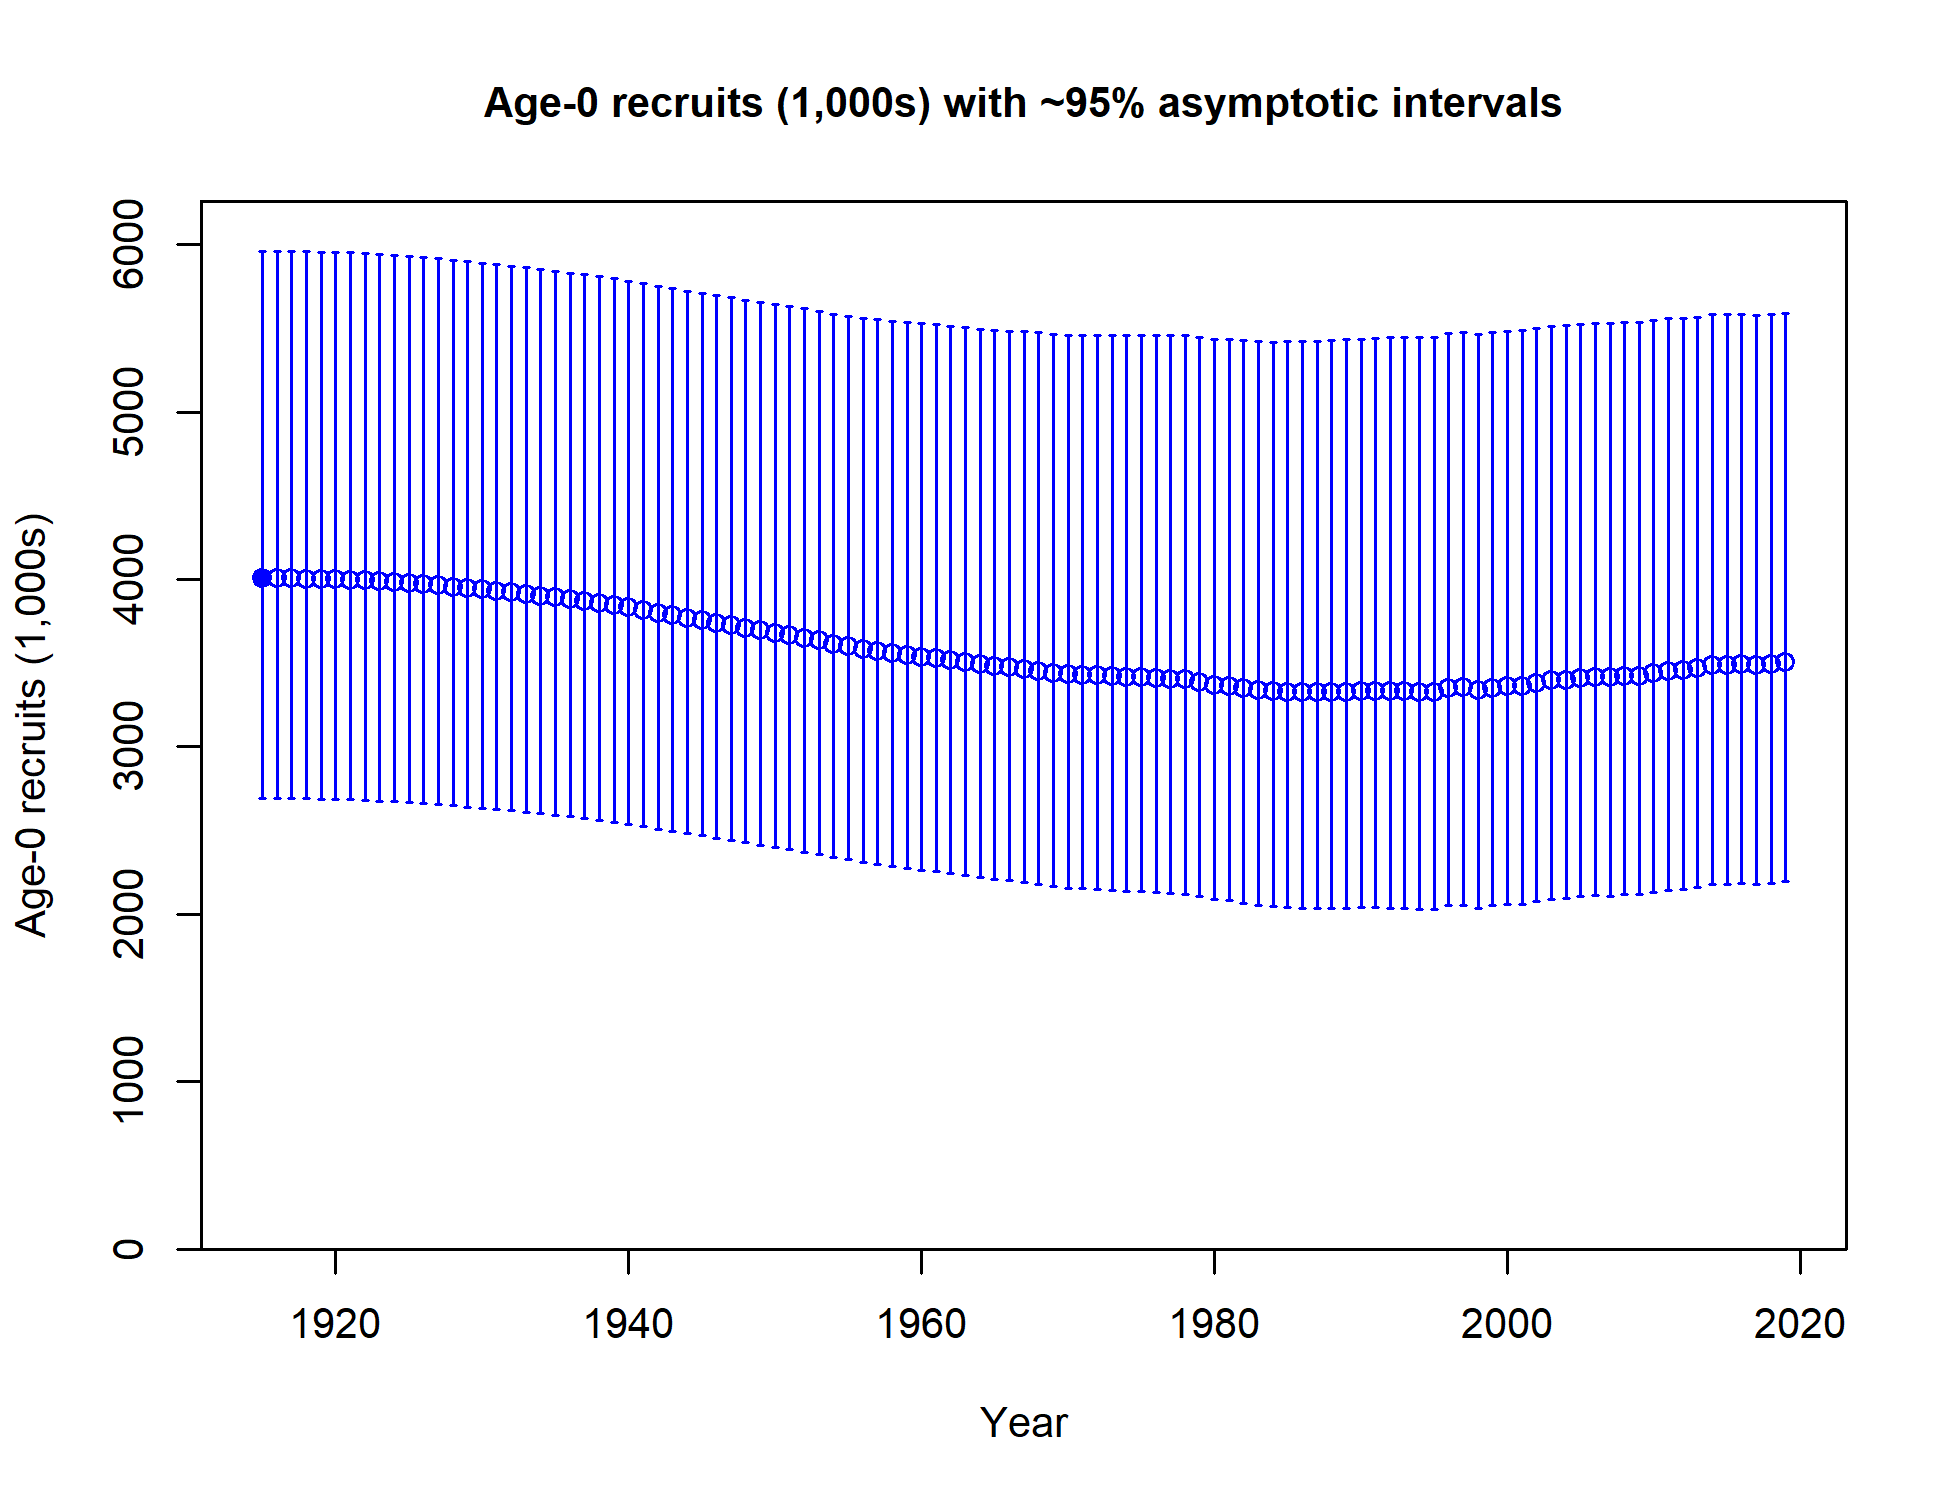
\includegraphics{r4ss/plots_mod1/ts11_Age-0_recruits_(1000s)_with_95_asymptotic_intervals.png}
\caption{Time series of estimated Big Skate recruitments for the
base-case model with 95\% confidence or credibility intervals.
\label{fig:Recruits_all}}
\end{figure}

\FloatBarrier

\hypertarget{exploitation-status}{%
\subsection*{Exploitation status}\label{exploitation-status}}
\addcontentsline{toc}{subsection}{Exploitation status}

Harvest rates estimated by the base model \ldots{}.. management target
levels (Table \ref{tab:SPR_Exploit_mod1} and Figure \ref{fig:SPR_all}).

\FloatBarrier

\begin{table}[ht]
\centering
\caption{Recent trend in spawning potential 
                                        ratio and exploitation for Big Skate in the model.  Fishing intensity is (1-SPR) 
                                        divided by 50\% (the SPR target) and exploitation 
                                        is F divided by F\textsubscript{SPR}.} 
\label{tab:SPR_Exploit_mod1}
\begin{tabular}{l>{\centering}p{1in}>{\centering}p{1.2in}>{\centering}p{1in}>{\centering}p{1.2in}}
  \hline
Year & Fishing intensity & \~{} 95\% confidence interval & Exploitation rate & \~{} 95\% confidence interval \\ 
  \hline
2009 & 0.00 & (0-0) & 0.00 & (0-0) \\ 
  2010 & 0.00 & (0-0) & 0.00 & (0-0) \\ 
  2011 & 0.00 & (0-0) & 0.00 & (0-0) \\ 
  2012 & 0.00 & (0-0) & 0.00 & (0-0) \\ 
  2013 & 0.00 & (0-0) & 0.00 & (0-0) \\ 
  2014 & 0.00 & (0-0) & 0.00 & (0-0) \\ 
  2015 & 0.00 & (0-0) & 0.00 & (0-0) \\ 
  2016 & 0.00 & (0-0) & 0.00 & (0-0) \\ 
  2017 & 0.00 & (0-0) & 0.00 & (0-0) \\ 
  2018 & 0.00 & (0-0) & 0.00 & (0-0) \\ 
   \hline
\end{tabular}
\end{table}

\FloatBarrier

\begin{figure}
\centering
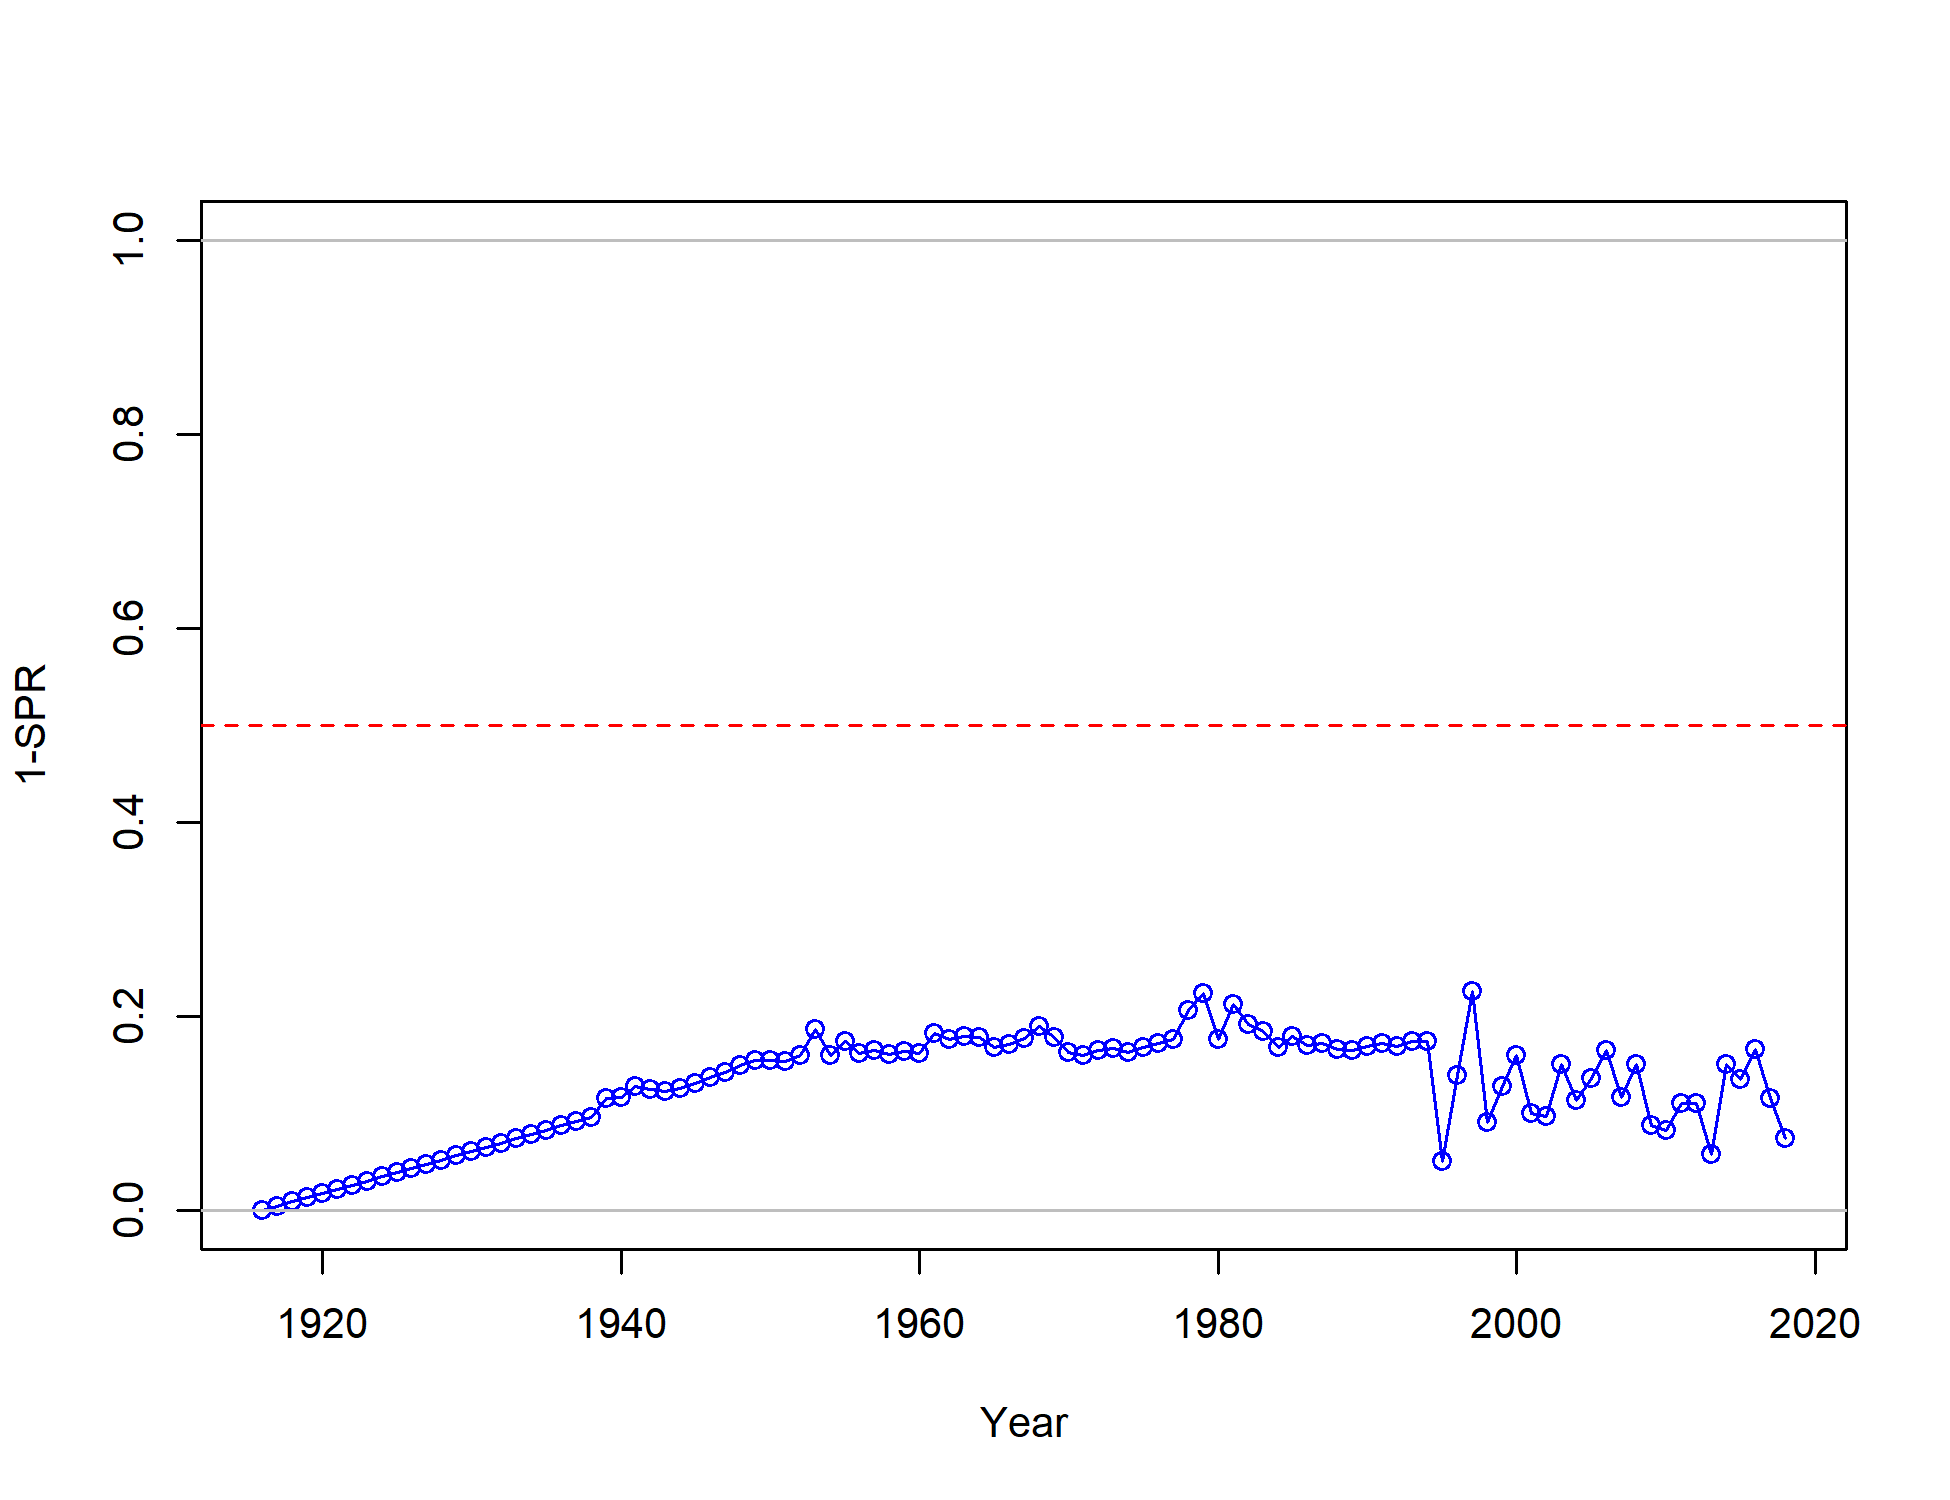
\includegraphics{r4ss/plots_mod1/SPR2_minusSPRseries.png}
\caption{Estimated spawning potential ratio (SPR) for the base-case
model. One minus SPR is plotted so that higher exploitation rates occur
on the upper portion of the y-axis. The management target is plotted as
a red horizontal line and values above this reflect harvests in excess
of the overfishing proxy based on the SPR\textsubscript{50\%} harvest
rate. The last year in the time series is 2018. \label{fig:SPR_all}}
\end{figure}

\FloatBarrier

\hypertarget{ecosystem-considerations}{%
\subsection*{Ecosystem Considerations}\label{ecosystem-considerations}}
\addcontentsline{toc}{subsection}{Ecosystem Considerations}

In this assessment, ecosystem considerations were not explicitly
included in the analysis.\\
This is primarily due to a lack of relevant data and results of analyses
(conducted elsewhere) that could contribute ecosystem-related
quantitative information for the assessment.

\hypertarget{reference-points}\)), and well above the minimum stock size
threshold (\(SB_{25\%}\)). The estimated relative depletion level for
the base model in 2019 is 99.8\% (95\% asymptotic interval: \(\pm\)
99.8\%-99.8\%, corresponding to an unfished spawning biomass of 70709.9
million eggs (95\% asymptotic interval: 70709.9-70709.9 million eggs) of
spawning biomass in the base model (Table \ref{tab:Ref_pts_mod1}).
Unfished age 1+ biomass was estimated to be 2,814 mt in the base case
model. The target spawning biomass (\(SB_{40\%}\)) is 2,834 million
eggs, which corresponds with an equilibrium yield of 5,906 mt.
Equilibrium yield at the proxy \(F_{MSY}\) harvest rate corresponding to
\(SPR_{50\%}\) is 5,070 mt (Figure \ref{fig:Yield_all}).

\FloatBarrier

\begin{table}[ht]
\centering
\caption{Summary of reference 
                                      points and management quantities for the 
                                      base case model.} 
\label{tab:Ref_pts_mod1}
\begin{tabular}{>{\raggedright}p{4.1in}>{\raggedleft}p{.62in}>{\raggedleft}p{.62in}>{\raggedleft}p{.62in}}
  \hline
\textbf{Quantity} & \textbf{Estimate} & \textbf{Low 2.5\%  limit} & \textbf{High 2.5\%  limit} \\ 
  \hline
Unfished spawning output (million eggs) & 7,086 & 7,086 & 7,086 \\ 
  Unfished age 1+ biomass (mt) & 2,814 & 2,814 & 2,814 \\ 
  Unfished recruitment ($R_{0}$) & 7,502 & 7,502 & 7,502 \\ 
  Spawning output(2018 million eggs) & 7,071 & 7,071 & 7,071 \\ 
  Depletion (2018) & 0.998 & 0.998 & 0.998 \\ 
  \textbf{$\text{Reference points based on } \mathbf{SB_{40\%}}$} &  &  &  \\ 
  Proxy spawning output ($B_{40\%}$) & 2,834 & 2,834 & 2,834 \\ 
  SPR resulting in $B_{40\%}$ ($SPR_{B40\%}$) & 0.625 & 0.625 & 0.625 \\ 
  Exploitation rate resulting in $B_{40\%}$ & 0.04 & 0.04 & 0.04 \\ 
  Yield with $SPR_{B40\%}$ at $B_{40\%}$ (mt) & 5,906 & 5,906 & 5,906 \\ 
  \textbf{\textit{Reference points based on SPR proxy for MSY}} &  &  &  \\ 
  Spawning output & 1,417 & 1,417 & 1,417 \\ 
  $SPR_{proxy}$ & 0.5 &  &  \\ 
  Exploitation rate corresponding to $SPR_{proxy}$ & 0.058 & 0.058 & 0.058 \\ 
  Yield with $SPR_{proxy}$ at $SB_{SPR}$ (mt) & 5,070 & 5,070 & 5,070 \\ 
  \textbf{\textit{Reference points based on estimated MSY values}} &  &  &  \\ 
  Spawning output at $MSY$ ($SB_{MSY}$) & 2,578 & 2,578 & 2,578 \\ 
  $SPR_{MSY}$ & 0.602 & 0.602 & 0.602 \\ 
  Exploitation rate at $MSY$ & 0.043 & 0.043 & 0.043 \\ 
  Dead Catch $MSY$ (mt) & 5,939 & 5,939 & 5,939 \\ 
  Retained Catch $MSY$ (mt) & 5,939 & 5,939 & 5,939 \\ 
   \hline
\end{tabular}
\end{table}

\FloatBarrier

\hypertarget{management-performance}{%
\subsection*{Management Performance}\label{management-performance}}
\addcontentsline{toc}{subsection}{Management Performance}

Table \ref{tab:mnmgt_perform}

\begin{table}[ht]
\centering
\caption{Recent trend in total catch and commercial 
                              landings (mt) relative to the management guidelines. 
                              Estimated total catch reflect the commercial landings 
                              plus the model estimated discarded biomass.} 
\label{tab:mnmgt_perform}
\scalebox{0.9}{
\begin{tabular}{>{\raggedleft}p{1in}>{\centering}p{1in}>{\centering}p{1in}>{\centering}p{1in}>{\centering}p{1in}}
  \hline
Year & OFL (mt; ABC prior to 2011) & ABC (mt) & ACL (mt; OY prior to 2011) & Estimated total catch (mt) \\ 
  \hline
\textbf{2007} & - & - & - & - \\ 
  \textbf{2008} & - & - & - & - \\ 
  \textbf{2009} & - & - & - & - \\ 
  \textbf{2010} & - & - & - & - \\ 
  \textbf{2011} & - & - & - & - \\ 
  \textbf{2012} & - & - & - & - \\ 
  \textbf{2013} & - & - & - & - \\ 
  \textbf{2014} & - & - & - & - \\ 
  \textbf{2015} & - & - & - & - \\ 
  \textbf{2016} & - & - & - & - \\ 
  \textbf{2017} & - & - & - & - \\ 
  \textbf{2018} & - & - & - & - \\ 
   \hline
\end{tabular}
}
\end{table}

\hypertarget{unresolved-problems-and-major-uncertainties}{%
\subsection*{Unresolved Problems and Major
Uncertainties}\label{unresolved-problems-and-major-uncertainties}}
\addcontentsline{toc}{subsection}{Unresolved Problems and Major
Uncertainties}

\FloatBarrier

\hypertarget{decision-table}{%
\subsection*{Decision Table}\label{decision-table}}
\addcontentsline{toc}{subsection}{Decision Table}

\begin{table}[ht]
\centering
\caption{Projections of potential OFL (mt) for 
                                        each model, using the base model forecast.} 
\label{tab:OFL_projection}
\begin{tabular}{lr}
  \hline
Year & OFL \\ 
  \hline
2019 & 158932.00 \\ 
  2020 & 149035.00 \\ 
  2021 & 141655.00 \\ 
  2022 & 136395.00 \\ 
  2023 & 132529.00 \\ 
  2024 & 129293.00 \\ 
  2025 & 126187.00 \\ 
  2026 & 122991.00 \\ 
  2027 & 119650.00 \\ 
  2028 & 116197.00 \\ 
  2029 & 112719.00 \\ 
  2030 & 109333.00 \\ 
   \hline
\end{tabular}
\end{table}
\begin{table}[ht]
\centering
\caption{Summary of 10-year 
                                             projections beginning in 2020 
                                             for alternate states of nature based on 
                                             an axis of uncertainty for the model.  Columns range over low, mid, and high
                                             states of nature, and rows range over different 
                                             assumptions of catch levels. An entry of "--" 
                                             indicates that the stock is driven to very low 
                                             abundance under the particular scenario.} 
\label{tab:Decision_table_mod1}
\scalebox{0.85}{
\begin{tabular}{l|cc|>{\centering}p{.7in}c|>{\centering}p{.7in}c|>{\centering}p{.7in}c}
   \multicolumn{3}{c}{}  &  \multicolumn{2}{c}{} 
                               & \multicolumn{2}{c}{\textbf{States of nature}} 
                               & \multicolumn{2}{c}{} \\
  \multicolumn{3}{c}{}  &  \multicolumn{2}{c}{Low M 0.05} 
                               & \multicolumn{2}{c}{Base M 0.07} 
                               &  \multicolumn{2}{c}{High M 0.09} \\
 \hline
 & Year & Catch & Spawning Output & Depletion & Spawning Output & Depletion & Spawning Output & Depletion \\ 
  \hline
 & 2019 & - & - & - & - & - & - & - \\ 
   & 2020 & - & - & - & - & - & - & - \\ 
   & 2021 & - & - & - & - & - & - & - \\ 
  40-10 Rule,  & 2022 & - & - & - & - & - & - & - \\ 
  Low M & 2023 & - & - & - & - & - & - & - \\ 
   & 2024 & - & - & - & - & - & - & - \\ 
   & 2025 & - & - & - & - & - & - & - \\ 
   & 2026 & - & - & - & - & - & - & - \\ 
   & 2027 & - & - & - & - & - & - & - \\ 
   & 2028 & - & - & - & - & - & - & - \\ 
   \hline
 & 2019 & - & - & - & - & - & - & - \\ 
   & 2020 & - & - & - & - & - & - & - \\ 
   & 2021 & - & - & - & - & - & - & - \\ 
  40-10 Rule & 2022 & - & - & - & - & - & - & - \\ 
   & 2023 & - & - & - & - & - & - & - \\ 
   & 2024 & - & - & - & - & - & - & - \\ 
   & 2025 & - & - & - & - & - & - & - \\ 
   & 2026 & - & - & - & - & - & - & - \\ 
   & 2027 & - & - & - & - & - & - & - \\ 
   & 2028 & - & - & - & - & - & - & - \\ 
   \hline
 & 2019 & - & - & - & - & - & - & - \\ 
   & 2020 & - & - & - & - & - & - & - \\ 
   & 2021 & - & - & - & - & - & - & - \\ 
  40-10 Rule, & 2022 & - & - & - & - & - & - & - \\ 
  High M & 2023 & - & - & - & - & - & - & - \\ 
   & 2024 & - & - & - & - & - & - & - \\ 
   & 2025 & - & - & - & - & - & - & - \\ 
   & 2026 & - & - & - & - & - & - & - \\ 
   & 2027 & - & - & - & - & - & - & - \\ 
   & 2028 & - & - & - & - & - & - & - \\ 
   \hline
 & 2019 & - & - & - & - & - & - & - \\ 
   & 2020 & - & - & - & - & - & - & - \\ 
   & 2021 & - & - & - & - & - & - & - \\ 
  Average & 2022 & - & - & - & - & - & - & - \\ 
  Catch & 2023 & - & - & - & - & - & - & - \\ 
   & 2024 & - & - & - & - & - & - & - \\ 
   & 2025 & - & - & - & - & - & - & - \\ 
   & 2026 & - & - & - & - & - & - & - \\ 
   & 2027 & - & - & - & - & - & - & - \\ 
   & 2028 & - & - & - & - & - & - & - \\ 
   \hline
\end{tabular}
}
\end{table}

\begin{sidewaystable}[ht]
\centering
\caption{Base case results summary.} 
\label{tab:base_summary}
\scalebox{0.6}{
\begin{tabular}{r>{\centering}p{1.1in}>{\centering}p{1.1in}>{\centering}p{1.1in}>{\centering}p{1.1in}>{\centering}p{1.1in}>{\centering}p{1.1in}>{\centering}p{1.1in}>{\centering}p{1.1in}>{\centering}p{1.1in}>{\centering}p{1.1in}}
  \hline
Quantity & 2010 & 2011 & 2012 & 2013 & 2014 & 2015 & 2016 & 2017 & 2018 & 2019 \\ 
  \hline
Landings (mt) &  &  &  &  &  &  &  &  &  &  \\ 
  Total Est. Catch (mt) &  &  &  &  &  &  &  &  &  &  \\ 
  OFL (mt) &  &  &  &  &  &  &  &  &  &  \\ 
  ACL (mt) &  &  &  &  &  &  &  &  &  &  \\ 
   \hline
(1-$SPR$)(1-$SPR_{50\%}$) &  0 &  0 &  0 &  0 &  0 &  0 &  0 &  0 &  0 &  \\ 
   \hline
Exploitation rate &  0 &  0 &  0 &  0 &  0 &  0 &  0 &  0 &  0 &  \\ 
  Age 1+ biomass (mt) & 2654110 & 2654240 & 2654360 & 2654400 & 2654430 & 2654570 & 2654490 & 2654470 & 2654390 & 2654450 \\ 
   \hline
Spawning Output & 70693.2 & 70697.5 & 70699.9 & 70702.4 & 70709.2 & 70708.7 & 70708.9 & 70706.0 & 70706.5 & 70709.9 \\ 
  ~95\% CI & (70693.2-70693.2) & (70697.5-70697.5) & (70699.9-70699.9) & (70702.4-70702.4) & (70709.2-70709.2) & (70708.7-70708.7) & (70708.9-70708.9) & (70706-70706) & (70706.5-70706.5) & (70709.9-70709.9) \\ 
   \hline
Depletion & 1 & 1 & 1 & 1 & 1 & 1 & 1 & 1 & 1 & 1 \\ 
  ~95\% CI & (0.998-0.998) & (0.998-0.998) & (0.998-0.998) & (0.998-0.998) & (0.998-0.998) & (0.998-0.998) & (0.998-0.998) & (0.998-0.998) & (0.998-0.998) & (0.998-0.998) \\ 
   \hline
Recruits & 749.57 & 749.59 & 749.60 & 749.61 & 749.64 & 749.63 & 749.63 & 749.62 & 749.62 & 749.64 \\ 
  ~95\% CI & (749.57 - 749.57) & (749.59 - 749.59) & (749.6 - 749.6) & (749.61 - 749.61) & (749.64 - 749.64) & (749.63 - 749.63) & (749.63 - 749.63) & (749.62 - 749.62) & (749.63 - 749.63) & (749.64 - 749.64) \\ 
   \hline
\end{tabular}
}
\end{sidewaystable}

\begin{figure}
\centering
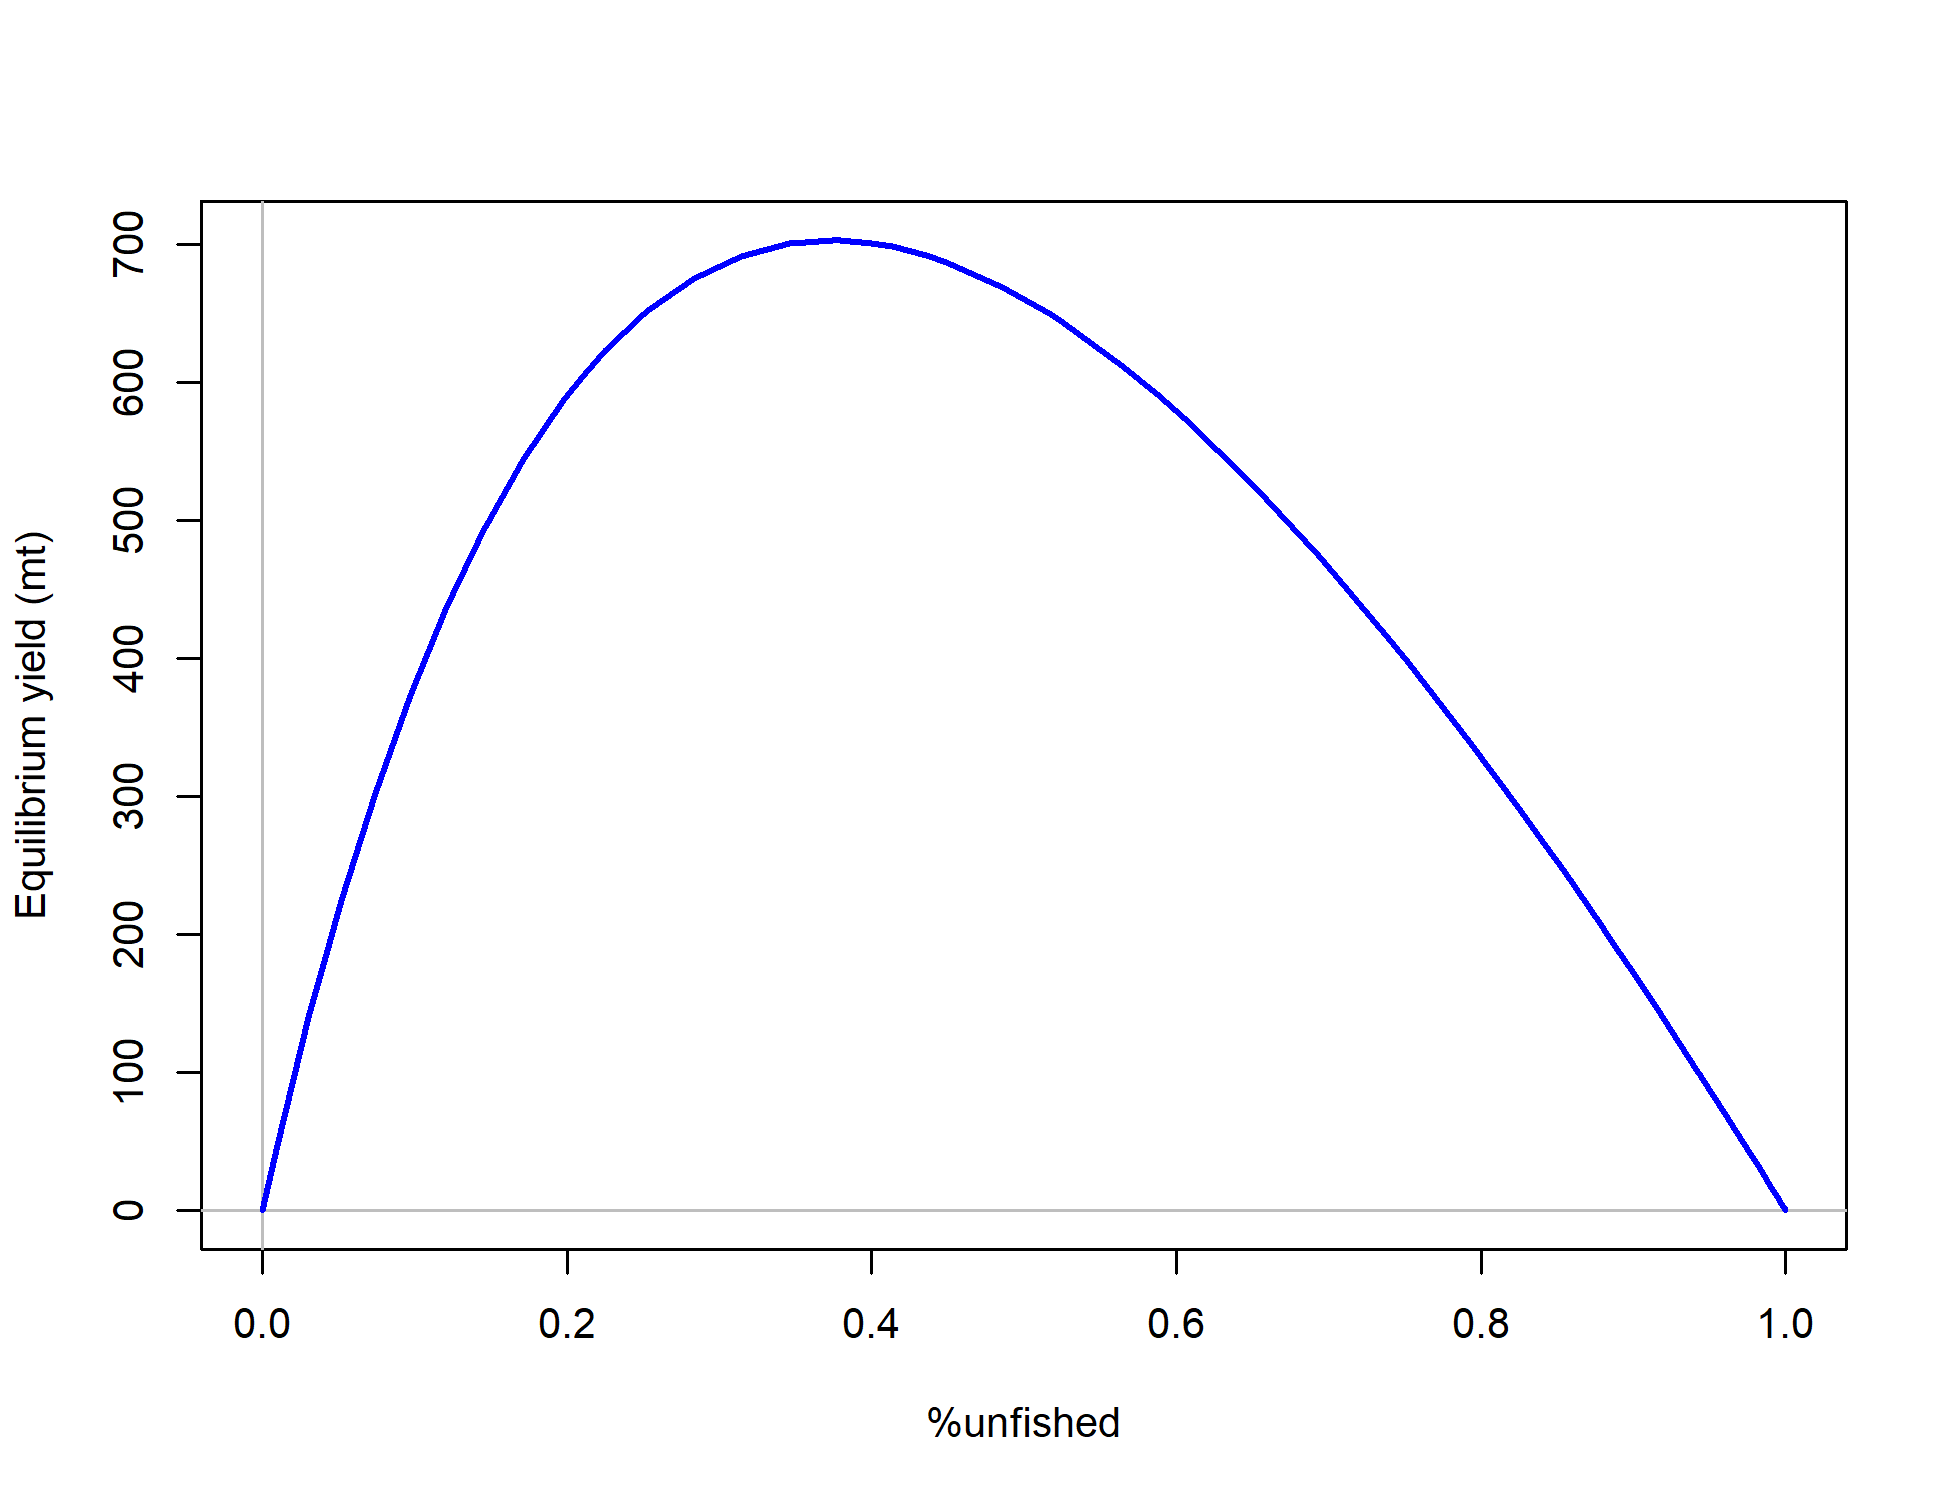
\includegraphics{r4ss/plots_mod1/yield1_yield_curve.png}
\caption{Equilibrium yield curve for the base case model. Values are
based on the 2018 fishery selectivity and with steepness fixed at 0.718.
\label{fig:Yield_all}}
\end{figure}

\FloatBarrier

\newpage

\hypertarget{research-and-data-needs}{%
\subsection*{Research and Data Needs}\label{research-and-data-needs}}
\addcontentsline{toc}{subsection}{Research and Data Needs}

We recommend the following research be conducted before the next
assessment:

\begin{enumerate}

\item \textbf{xxxx}: 

\item \textbf{xxxx}:

\item \textbf{xxxx}:

\item \textbf{xxxx}:

\item \textbf{xxxx}:

\end{enumerate}

\FloatBarrier

\newpage
\renewcommand{\thefigure}{\arabic{figure}}
\renewcommand{\thetable}{\arabic{table}}
\setcounter{figure}{0}
\setcounter{table}{0}

\newpage
\setcounter{page}{1}
\renewcommand{\thefigure}{\alph{figure}}
\renewcommand{\thetable}{\alph{table}}

\hypertarget{introduction}{%
\section{Introduction}\label{introduction}}

\hypertarget{distribution-and-life-history}{%
\subsection{Distribution and Life
History}\label{distribution-and-life-history}}

Big Skate (\emph{Raja binoculata}) is the largest of the skate species
in North America with a documented maximum length of 244 cm total length
and a maximum weight of 91 kg (Eschmeyer, et al.~1983). The species name
``binoculata'' (two-eyed) refers to the prominent ocellus at the base of
each pectoral fin. Big skate range from the Bering Sea to Cedros Island
in Baja California, but are uncommon south of Pt. Conception. Big skate
have a shallow depth distribution of 3-800 m, but are most common in the
3-110 m depth zone. Big Skate are observed in progressively shallower
water in the northern parts of its range. They occur in coastal bays,
estuaries, and over the continental shelf, usually on sandy or muddy
bottoms, but occasionally on low strands of kelp.

Skates are the largest and most widely distributed group of batoid fish
with approximately 245 species ascribed to two families (Ebert and
Compagno 2007; McEachran 1990). Skates are benthic fish that are found
in all coastal waters but are most common in cold temperatures and polar
waters (Ebert and Compagno 2007).

There are about eleven species of skates from either of three genera
(Amblyraja, Bathyraja, and Raja) present in the Northeast Pacific Ocean
off California, Oregon and Washington (Ebert 2003). Of that number, just
three species (Longnose Skate, \emph{Raja rhina}; Big Skate, \emph{Raja
binoculata}; and Sandpaper Skate, \emph{Bathyraja interrupta}) make up
over 95 percent of West Coast Groundfish Bottom Trawl Survey (WCGBTS)
catches in terms of biomass and numbers, with the Longnose Skate leading
in both categories (with 62 percent of biomass and 56 percent of
numbers).

Mating has been observed with distinct pairing with embrace. Big Skate
are oviparous and lay horned egg cases up to a foot in length with up to
seven embryos per egg case (Eschmeyer, et al.1983). The female deposits
her eggs in pairs on sandy or muddy flats; there is no discrete
breedingseason and egg-laying occurs year-round (Ebert 2003). Females
may use discrete spawning beds, as large numbers of egg cases have been
found in certain localized areas (IUCN/SSC Shark Specialist Group 2005).
The young emerge after 9 months and measure 18--23 cm (7--9 in).

Female Big Skates mature at 1.3--1.4 m (4 ft 3 in--4 ft 7 in) long and
12--13 years old, while males mature at 0.9--1.1 m (2 ft 11 in--3 ft 7
in) long and seven to eight years old (Bester 2009). The growth rate of
Big Skates in the Gulf of Alaska are comparable to those off California,
but differ from those off British Columbia. The lifespans of big skates
off Alaska are up to 15 years, while those off British Columbia are up
to 26 years.

Big Skates are usually seen buried in sediment with only their eyes
showing. They feed on polychaete worms, mollusks, crustaceans, and small
benthic fishes. Polychaetes and mollusks comprise a slightly greater
percentage of the diet of younger individuals. A known predator of big
skates is the Broadnose Sevengill Shark (\emph{Notorhynchus
cepedianus}); the eyespots on the skates' wings are believed to serve as
decoys to confuse predators. Juvenile Northern Elephant Seals
(\emph{Mirounga angustirostris}) are known to consume the egg cases of
the Big Skate. Known parasites of the Big Skate include the copepod
\emph{Lepeophtheirus cuneifer}.

\hypertarget{early-life-history}{%
\subsection{Early Life History}\label{early-life-history}}

\hypertarget{map}{%
\subsection{Map}\label{map}}

A map showing the scope of the assessment and depicting boundaries for
fisheries or data collection strata is provided in Figure
\ref{fig:boundary_map}.

\hypertarget{ecosystem-considerations-1}{%
\subsection{Ecosystem Considerations}\label{ecosystem-considerations-1}}

In this assessment, ecosystem considerations were not explicitly
included in the analysis. This is primarily due to a lack of relevant
data and results of analyses (conducted elsewhere) that could contribute
ecosystem-related quantitative information for the assessment.

\hypertarget{fishery-information}{%
\subsection{Fishery Information}\label{fishery-information}}

\hypertarget{stock-status-and-management-history}{%
\subsection{Stock Status and Management
History}\label{stock-status-and-management-history}}

Big Skate are caught in commercial and recreational fisheries on the
West Coast using line and trawl gears. They are commercially utilized to
a limited extent by removing the pectoral fins (skate wings) for sale in
fresh fish markets.

Big Skate were managed in the Other Fish complex until 2015 when they
were designated an Ecosystem Component (EC) species. Catches of Big
Skate are estimated to have averaged 95 mt from 2007--2011, along with
large landings of Unspecified Skate. Analysis of Oregon port sampling
data indicates that about 98 percent of the recent Unspecified Skate
landings in Oregon were comprised of Big Skate. Such large landings
indicates targeting of Big Skate has occurred and an EC designation was
not warranted. Based on this evidence, Big Skate was redesignated as an
actively-managed species in the fishery. Big skate have been managed
with stock-specific harvest specifications since 2017.

The recent OFL of 541 mt was calculated by applying approximate MSY
harvest rates to estimates of stock biomass from the Northwest Fisheries
Science Center (NWFSC) West Coast Bottom Trawl Survey. This survey-based
biomass estimate is likely underestimated since Big Skate are
distributed to the shore and no West Coast trawl surveys have been
conducted shallower than 55 m. This adds a level of precaution to the
management of Big Skate with stock-specific management reducing
management uncertainty and the risk of overfishing the stock.

There has been consideration for managing Big Skate in a complex with
Longnose Skate, the other actively-managed West Coast skate species, but
the two species have disparate distributions and fishery interactions
(Longnose Skate is much more deeply distributed than Big Skate) and that
option was not endorsed. The Council has chosen to set the Annual Catch
Limit (ACL) equal to the Allowable Biological Catch (ABC) with a buffer
for management uncertainty (P* of 0.45).

\hypertarget{management-performance-1}{%
\subsection{Management Performance}\label{management-performance-1}}

Table \ref{tab:mnmgt_perform}

\hypertarget{fisheries-off-mexico-or-canada}{%
\subsection{Fisheries Off Mexico or
Canada}\label{fisheries-off-mexico-or-canada}}

\newpage

\#Assessment

\#\#Data Data used in the Big Skate assessment are summarized in Figure
\ref{fig:data_plot}. Descriptions of the data sources are in the
following sections.

\#\#\#Commercial Fishery Landings

Catch reconstructions for WA, OR, and CA Tribal catch in WA

\#\#\#Commercial Discards

Estimated discards

\#\#\#Commercial Fishery Length and Age Data

The input sample sizes were calculated via the Stewart Method (Ian
Stewart, personal communication, IPHC):

\begin{centering}

Input effN = $N_{\text{trips}} + 0.138 * N_{\text{fish}}$ if $N_{\text{fish}}/N_{\text{trips}}$ is $<$ 44

Input effN = $7.06 * N_{\text{trips}}$ if $N_{\text{fish}}/N_{\text{trips}}$ is $\geq$ 44

\end{centering}

\#\#\#Sport Fishery Removals and Discards

Biological samples from the recreational fleets are described in the
sections below.

\#\#\#Fishery-Dependent Indices of Abundance

\textbf{Data Source 1}

\emph{Data Source 1 Index Standardization}

\emph{Data Source 1 Length Composition}

\textbf{Data Source 2}

\textbf{Data Source 3}

\#\#\#Fishery-Independent Data Sources

\textbf{Alaska Fisheries Science Center (AFSC) Triennial Shelf Survey}\\
Research surveys have been used since the 1970s to provide
fishery-independent information about the abundance, distribution, and
biological characteristics of Big Skate. A coast-wide survey was
conducted in 1977 (Gunderson, Donald Raymond and Sample, Terrance M.
\protect\hyperlink{ref-Gunderson1980}{n.d.}) by the Alaska Fisheries
Science Center, and repeated every three years through 2001. The final
year of this survey, 2004, was conducted by the NWFSC according to the
AFSC protocol. We refer to this as the \textbf{Triennial Survey}.

The survey design used equally-spaced transects from which searches for
tows in a specific depth range were initiated. The depth range and
latitudinal range was not consistent across years, but all years in the
period 1980-2004 included the area from 40\(^\circ\) 10'N north to the
Canadian border and a depth range that included 55-366 meters, which
spans the range where the vast majority of Big Skate encountered in all
trawl surveys. Therefore the index was based on this depth range. The
survey as conducted in 1977 had incomplete coverage and is not believe
to be comparable to the later years, and is not used in the index.

An index of abundance was estimated based on the VAST delta-GLMM model
as described for the NWFSC Combo Index above. In this case as well, Q-Q
plots indicated slightly better performance of the gamma over lognormal
models for positive tows (Figure \ref{fig:VAST_QQ}).

\textbf{Northwest Fisheries Science Center West Coast Groundfish Bottom
Trawl Survey}

In 2003, the NWFSC took over an ongoing slope survey the AFSC had been
conducting, and expanded it spatially to include the continental shelf.
This survey, referred to in this document as the \textbf{NWFSC Combo
Survey}, has been conducted annually since. It uses a random-grid design
covering the coastal waters from a depth of 55 m to 1,280 m from
late-May to early-October (Bradburn, M.J. and Keller, A.A and Horness,
B.H. \protect\hyperlink{ref-Bradburn2011}{n.d.} , Keller, A.A. and
Wallace, J.R. and Methot, R.D.
\protect\hyperlink{ref-Keller2017}{n.d.}). Four chartered industry
vessels are used each year (with the exception of 2013 when the U.S.
federal-government shutdown curtailed the survey). Yellowtail catches in
the NWFSC Combo Survey are shown in \ref{fig:assess_region_map2}.

The data from the NWFSC Combo survey was analyzed using a
spatio-temporal delta-model (Thorson, J. T. and Shelton, A. O. and Ward,
E. J. and Skaug, H. J. \protect\hyperlink{ref-Thorson2015}{n.d.}),
implemented as an R package VAST ({\textbf{???}}) and publicly available
online (\url{https://github.com/James-Thorson/VAST}). Spatial and
spatio-temporal variation is specifically included in both encounter
probability and positive catch rates, a logit-link for encounter
probability, and a log-link for positive catch rates. Vessel-year
effects were included for each unique combination of vessel and year in
the database.

\emph{Data Source 1 Index Standardization} VAST

\emph{Data Source 1 Length Composition}

\textbf{Triennial Survey} \emph{Data Source 2 Index Standardization}
VAST

\newpage

\#\#\#Biological Parameters and Data

\textbf{Measurement Details and Conversion Factors}

Disc width to total length (estimated by Ian on Apr 15, similar to Ebert
2008 estimates for Alaska) L = 1.3399 * W estimated from 95 samples from
WCGBTS where both measurements collected (R-squared = 0.9983). Little
sex difference observed, so using single relationship for both sexes.
Inter-spiracle width to total length from Downs \& Cheng (2013): L =
12.111 + 9.761\emph{ISW (females) L = 3.824 + 10.927}ISW (males)

Love et al.~(\protect\hyperlink{ref-Love1987}{n.d.})

\textbf{Length and Age Compositions}

Length comps (some based on widths)

WCGBTS Lengths from all years except 2006 and 2007 Widths in 2006 and
2007

Triennial Survey Sample sizes: 3 in 1998 (all widths), 84 in 2001 (3
widths, 81 lengths), 100 in 2004 (all lengths) Triennial survey About
90+ samples in each of 2001 and 2004 Only 3 unsexed fish from 1998

Commercial fisheries In process Discard comps from 2010-2015

Length compositions were provided from the following sources:

\begin{itemize}[noitemsep,nolistsep,topsep=0pt]
  \item Source 1 (\emph{type, e.g., commercial dead fish, research, recreational}, yyyy-yyyy)    
  \item Source 2 (\emph{type}, yyyy-yyyy)    
  \item Source 3 (\emph{research}, yyyy, yyyy, yyyy, yyyy) 
\end{itemize}

The length composition of all fisheries aggregated across time by fleet
is in Figure \ref{fig:comp_lendat_aggregated_across_time}. Descriptions
and details of the length composition data are in the above section for
each fleet or survey.

\vspace{.5cm}

\textbf{Age Structures}

von Bertalanffy growth curve ({\textbf{???}}),
\(L_i = L_{\infty}e^{(-k[t-t_0])}\), where \(L_i\) is the length (cm) at
age \(i\), \(t\) is age in years, \(k\) is rate of increase in growth,
\(t_0\) is the intercept, and \(L_{\infty}\) is the asymptotic length.

Ages WCGBTS Currently only 333 ages from 2010 present in data warehouse
as of Apr 15 Patrick submitting an 300 additional ages from 2016 and
2017 to Beth on Apr 2 and promised further additions during the week of
Apr 15.

Triennial Survey No ages

Commercial fisheries 2009 samples from WA were stratified by length, so
should be treated as conditionals

\vspace{.5cm}

\textbf{Aging Precision and Bias}

\vspace{.5cm}

\textbf{Weight-Length}

Estimated by Ian based on WCGBT samples (n = 1159) using code in
/R/growth\_plots.R Weight = 7.4924e-06 * Length \^{} 2.9925

\vspace{.5cm}

\textbf{Sex Ratio, Maturity, and Fecundity}

Estimated by Melissa Head from port samplers samples (n = 278, of which
241 were from OR and 37 from WA). 24 were mature.

Code is in /maturity/Longnose\_BigSkate\_maturity.r

Parameter estimates: L50\% = 149.5858, Slope parameter for SS = -0.13358

Adding 55 additional samples from the WCGBTS (of which only 4 were
mature) changes the parameter estimate to L50\% = 148.2453, Slope =
-0.13155

\vspace{.5cm}

\textbf{Natural Mortality}

The Hamel prior for M is lognormal(ln(5.4/max age),.438), which based on
1 age-15 fish out of 1034 observed in the WCGBTS results in lognormal(
-1.021651, 0.438)

If it needs to be fixed, it should be set to M = 5.4/max age = 5.4/15 =
0.36

\vspace{.5cm}

\#\#\#Environmental or Ecosystem Data Included in the Assessment In this
assessment, neither environmental nor ecosystem considerations were
explicitly included in the analysis. This is primarily due to a lack of
relevant data and results of analyses (conducted elsewhere) that could
contribute ecosystem-related quantitative information for the
assessment.

\newpage

\#\#Previous Assessments

\#\#\#History of Modeling Approaches Used for this Stock

Deriving estimates of OFL for species in the ``Other Fish'' complex or
potential alternative complexes

The current ``Other Fish'' complex and proposed alternatives include a
number of species for which estimates of OFL contributions are not
available from stock assessments or data-poor methods. Four of the
species had OFL contributions for the 2013--2014 management cycle
calculated by applying approximate MSY harvest rates to estimates of
stock biomass from the NWFSC West Coast Bottom Trawl Survey (Bradburn et
al., 2012). This approach is described in detail in Cope et al.~(2012).

\#\#\#yyyy Assessment Recommendations

\begin{description}[style=unboxed]

  \item[Recommendation 1: ] \hfill \\

   STAT response: xxxxx

\item[Recommendation 2: ] \hfill \\

  STAT response: xxxxx

\item[Recommendation 3: ] \hfill \\

  STAT response: xxxx

  
\end{description}

\#\#Model Description

\#\#\#Transition to the Current Stock Assessment

\#\#\#Summary of Data for Fleets and Areas There are xxx fleets in the
base model. They include:

\emph{Commercial}: The commercial fleets include \ldots{}

\emph{Recreational}: The recreational fleets include \ldots{}

\emph{Research}: There are xx sources of fishery-independent data
available \ldots{}

\#\#\#Other Specifications

\#\#\#Modeling Software The STAT team used Stock Synthesis 3 version
3.30.05.03 by Dr.~Richard Methot at the NWFSC. This most recent version
was used, since it included improvements and corrections to older
versions. The r4SS package (GitHub release number v1.27.0) was used to
post-processing output data from Stock Synthesis.

\#\#\#Data Weighting

\#\#\#Priors The log-normal prior for female natural mortality were
based on a meta-analysis completed by Hamel
(\protect\hyperlink{ref-Hamel2015}{n.d.}), as described under ``Natural
Mortality.'' Female natural mortality was fixed at the median of the
prior, 0.xxx for an assumed maximum age of xx. An uninformative prior
was used for the male offset natural mortality, which was estimated.

The prior for steepness (\emph{h}) assumes a beta distribution with
parameters based on an update for the Thorson-Dorn rockfish prior (Dorn,
M. and Thorson, J., pers. comm.), which was endorsed by the Science and
Statistical Committee in 2018. The prior is a beta distribution with
\(mu\)=0.xxx and \(sigma\)=0.xxx. Steepness is fixed in the base model
at the mean of the prior. The priors were applied in sensitivity
analyses where these parameters were estimated.

\#\#\#Estimated and Fixed Parameters A full list of all estimated and
fixed parameters is provided in Tables \ref{tab:model_params}.

The base model has a total of xxx estimated parameters in the following
categories:

\begin{itemize}
  \item xxx,
  \item xxx
  \item xxx, and
  \item xxx selectivity parameters
\end{itemize}

The estimated parameters are described in greater detail below and a
full list of all estimated and parameters is provided in Table
\ref{tab:model_params}.

\emph{Growth.}

\emph{Natural Mortality.}

\emph{Selectivity.}

\emph{Other Estimated Parameters.}

\emph{Other Fixed Parameters.}

\#\#Model Selection and Evaluation \#\#\#Key Assumptions and Structural
Choices

\#\#\#Alternate Models Considered

\#\#\#Convergence

\#\#Response to the Current STAR Panel Requests

\begin{description}[style=sameline]

\item[Request No. 1: ] \hfill \\
  
\textbf{Rationale:} xxx   
    
\textbf{STAT Response:} xxx


\item[Request No. 2: ] \hfill \\


\textbf{Rationale:} xxx 


\textbf{STAT Response:} xxx
    

\item[Request No. 3: ] \hfill \\

\textbf{Rationale:} x.  
    
  
\textbf{STAT Response:} xxx

\item[Request No. 4: ] \hfill \\

\textbf{Rationale:} xxx 
    
    
\textbf{STAT Response:} xxx


\item[Request No. 5: ] \hfill \\

\textbf{Rationale:} xxx
  
\textbf{STAT Response:} xxx  
    


\end{description}

\#\#Base Case Model Results The following description of the model
results reflects a base model that incorporates all of the changes made
during the STAR panel (see previous section). The base model parameter
estimates and their approximate asymptotic standard errors are shown in
Table \ref{tab:model_params} and the likelihood components are in Table
\ref{tab:like_components}. Estimates of derived reference points and
approximate 95\% asymptotic confidence intervals are shown in Table
\ref{tab:Ref_pts_mod1}. Time-series of estimated stock size over time
are shown in Table \ref{tab:Timeseries_mod1}.

\#\#\#Parameter Estimates

The additional survey variability (process error added directly to each
year's input variability) for all surveys was estimated within the
model.

(Figure
\ref{fig:ts11_Age-0_recruits_(1000s)_with_95_asymptotic_intervals} ).

The stock-recruit curve \ldots{} Figure \ref{fig:SR_curve2} with
estimated recruitments also shown.

\#\#\#Fits to the Data Model fits to the indices of abundance, fishery
length composition, survey length composition, and conditional
age-at-length observations are all discussed below.

\#\#\#Uncertainty and Sensitivity Analyses A number of sensitivity
analyses were conducted, including:

\begin{enumerate}

  \item Sensitivity 1
  
  \item Sensitivity 2
  
  \item Sensitivity 3
  
  \item Sensitivity 4
  
  \item Sensitivity 5, etc/
  
  
\end{enumerate}

\#\#\#Retrospective Analysis

\#\#\#Likelihood Profiles

\#\#\#Reference Points Reference points were calculated using the
estimated selectivities and catch distribution among fleets in the most
recent year of the model, (2017). Sustainable total yield (landings plus
discards) were 5,070 mt when using an \(SPR_{50\%}\) reference harvest
rate and with a 95\% confidence interval of 5,070 mt based on estimates
of uncertainty. The spawning biomass equivalent to 40\% of the unfished
level (\(SB_{40\%}\)) was 2,834 mt.

(Figure
\ref{fig:ts7_Spawning_biomass_(mt)_with_95_asymptotic_intervals_intervals}

The 2018 spawning biomass relative to unfished equilibrium spawning
biomass is above/below the target of 40\% of unfished levels (Figure
\ref{fig:ts9_Spawning_depletion_with_95_asymptotic_intervals_intervals}).
The relative fishing intensity, \((1-SPR)/(1-SPR_{50\%})\), has been xxx
the management target for the entire time series of the model.

Table \ref{tab:Ref_pts_mod1} shows the full suite of estimated reference
points for the base model and Figure \ref{fig:yield1_yield_curve} shows
the equilibrium curve based on a steepness value xxx.

\newpage

\#Harvest Projections and Decision Tables The forecasts of stock
abundance and yield were developed using the final base model, with the
forecasted projections of the OFL presented in Table
\ref{tab:OFL_projection}.

The forecasted projections of the OFL for each model are presented in
Table \ref{tab:Decision_table_mod1}.

\newpage

\#Regional Management Considerations \newpage

\#Research Needs There are a number of areas of research that could
improve the stock assessment for Big Skate. Below are issues identified
by the STAT team and the STAR panel:

\begin{enumerate}

\item \textbf{xxxx}: 

\item \textbf{xxxx}:

\item \textbf{xxxx}:

\item \textbf{xxxx}:

\item \textbf{xxxx}:

\end{enumerate}

\#Acknowledgments

\newpage
\FloatBarrier
\newpage

\FloatBarrier

\FloatBarrier

\FloatBarrier
\newpage

\newpage
\FloatBarrier

\FloatBarrier

\FloatBarrier

\FloatBarrier

\newpage

\FloatBarrier

\newpage

\#Figures

\begin{figure}
\centering
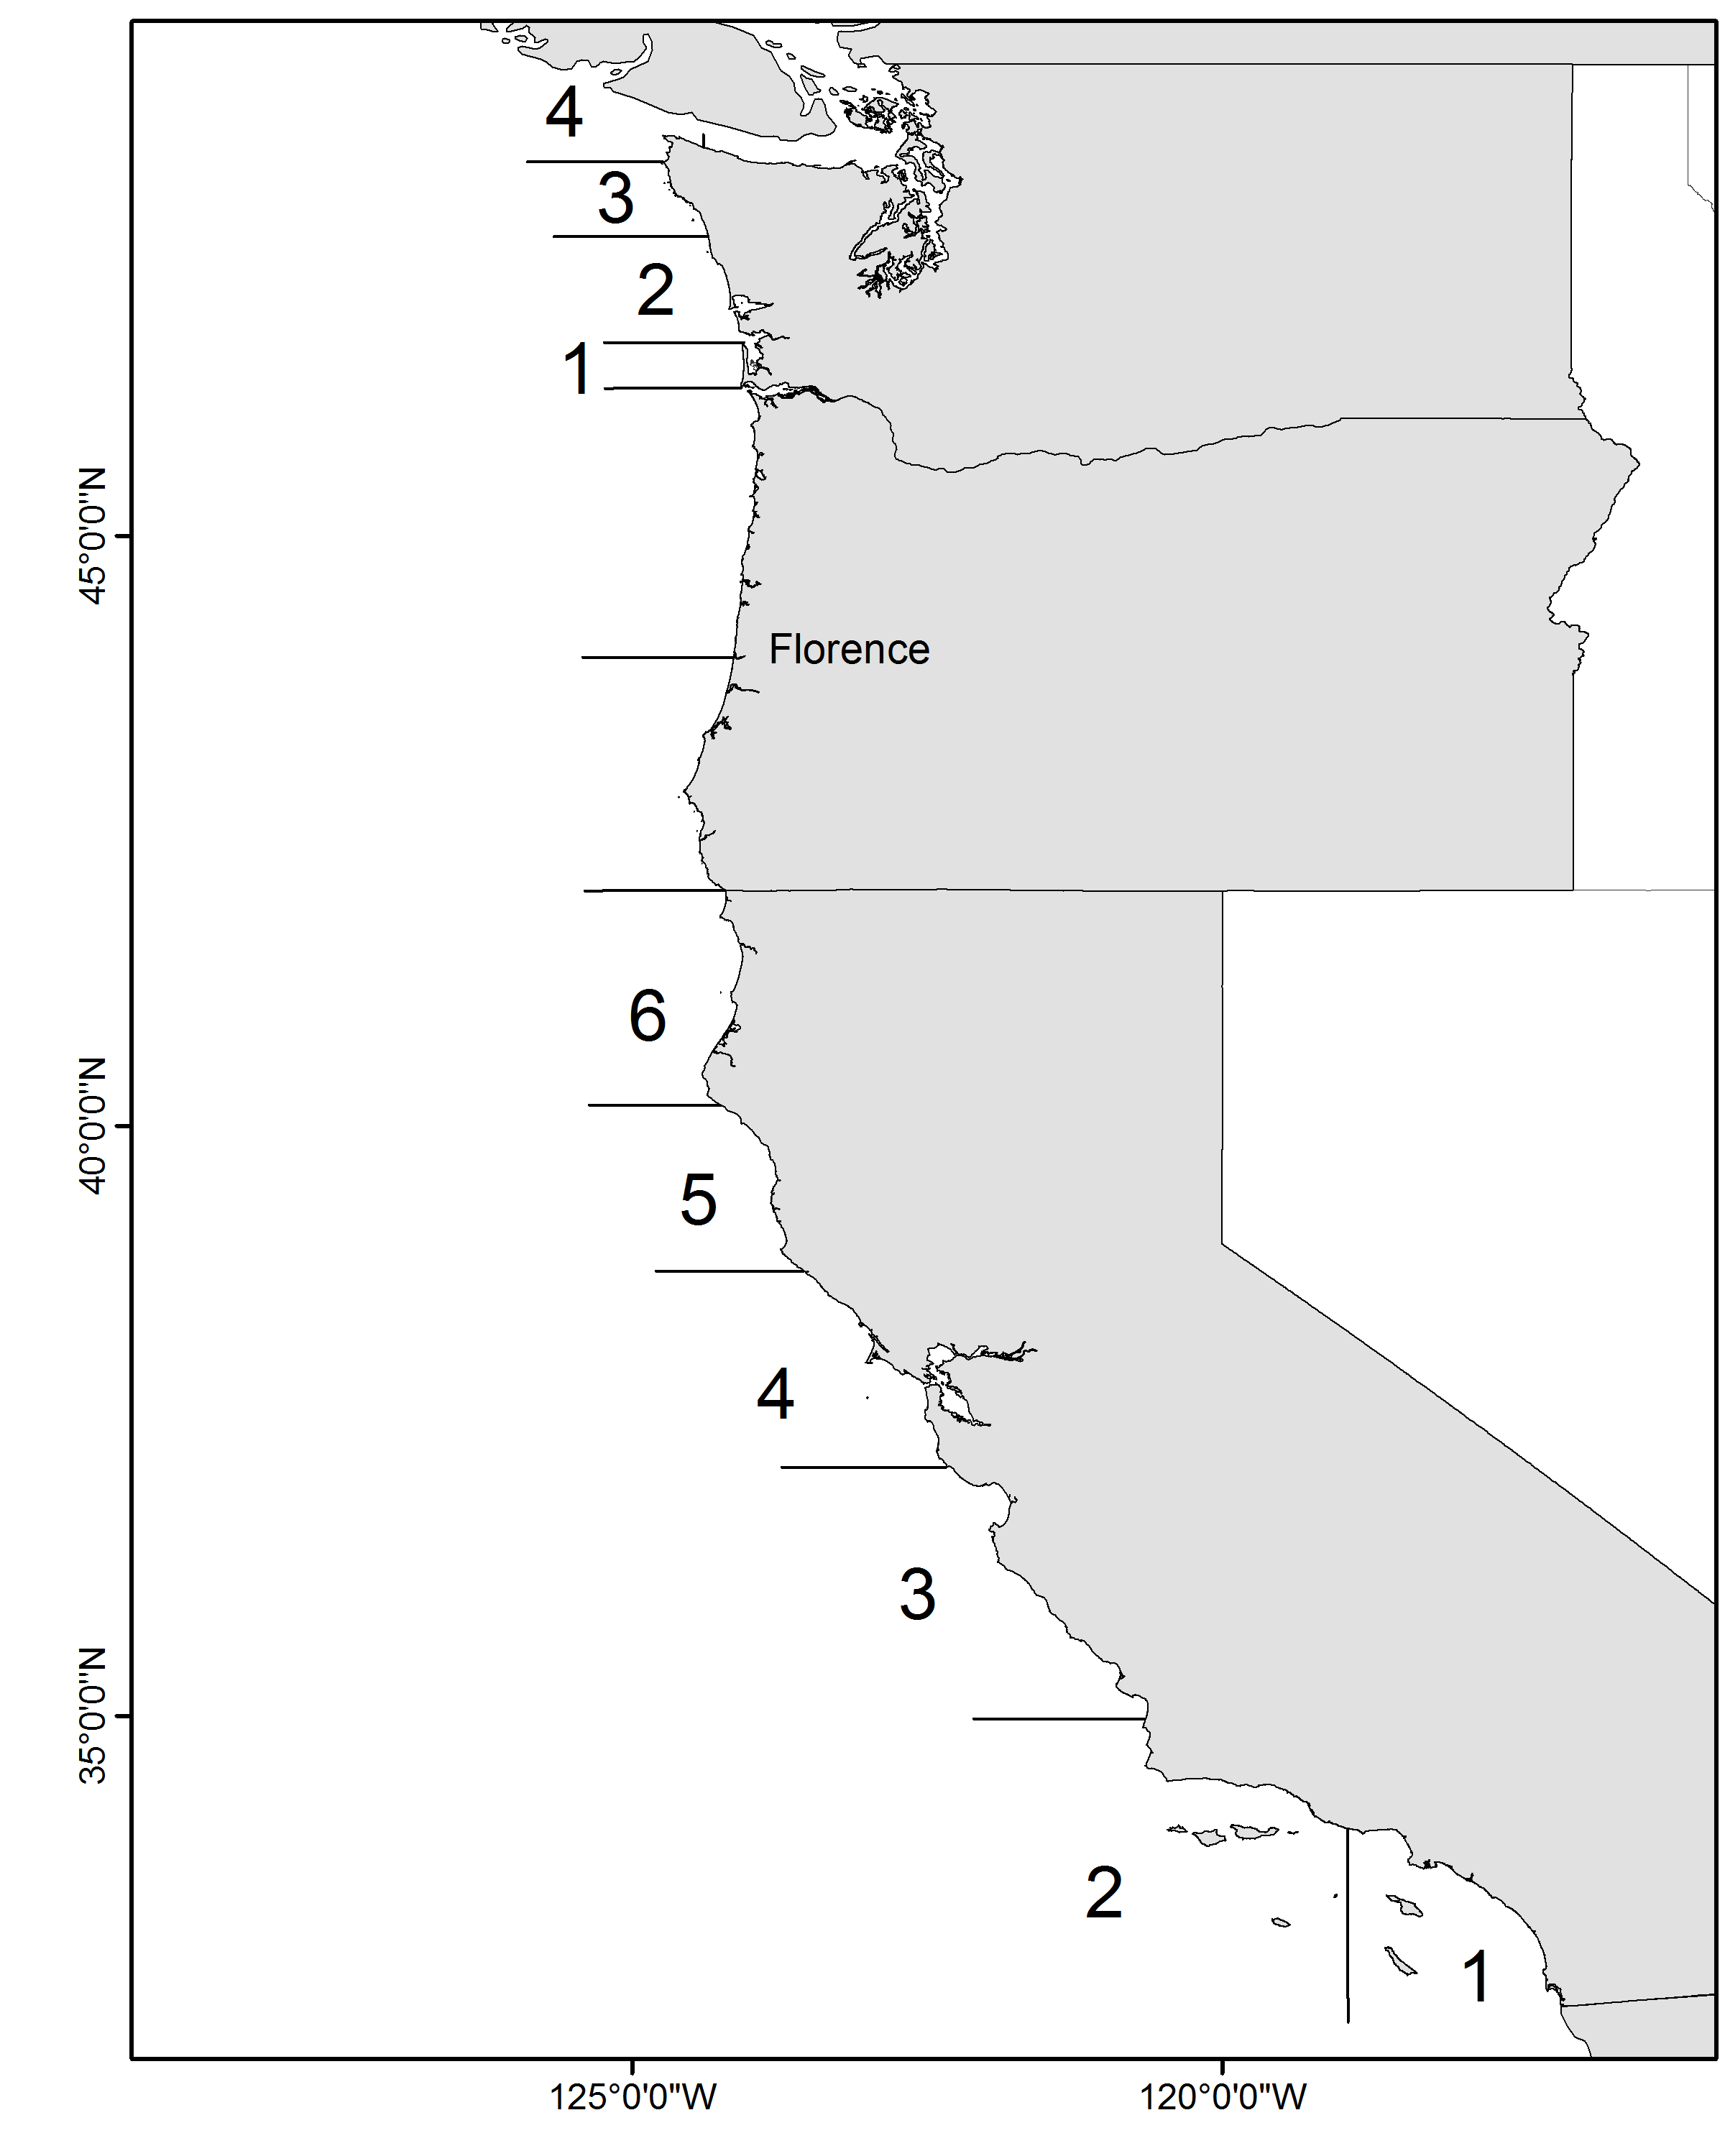
\includegraphics{Figures/boundary_map.png}
\caption{Map showing the state boundary lines for management of the
recreational fishing fleets \label{fig:boundary_map}}
\end{figure}

\begin{figure}
\centering
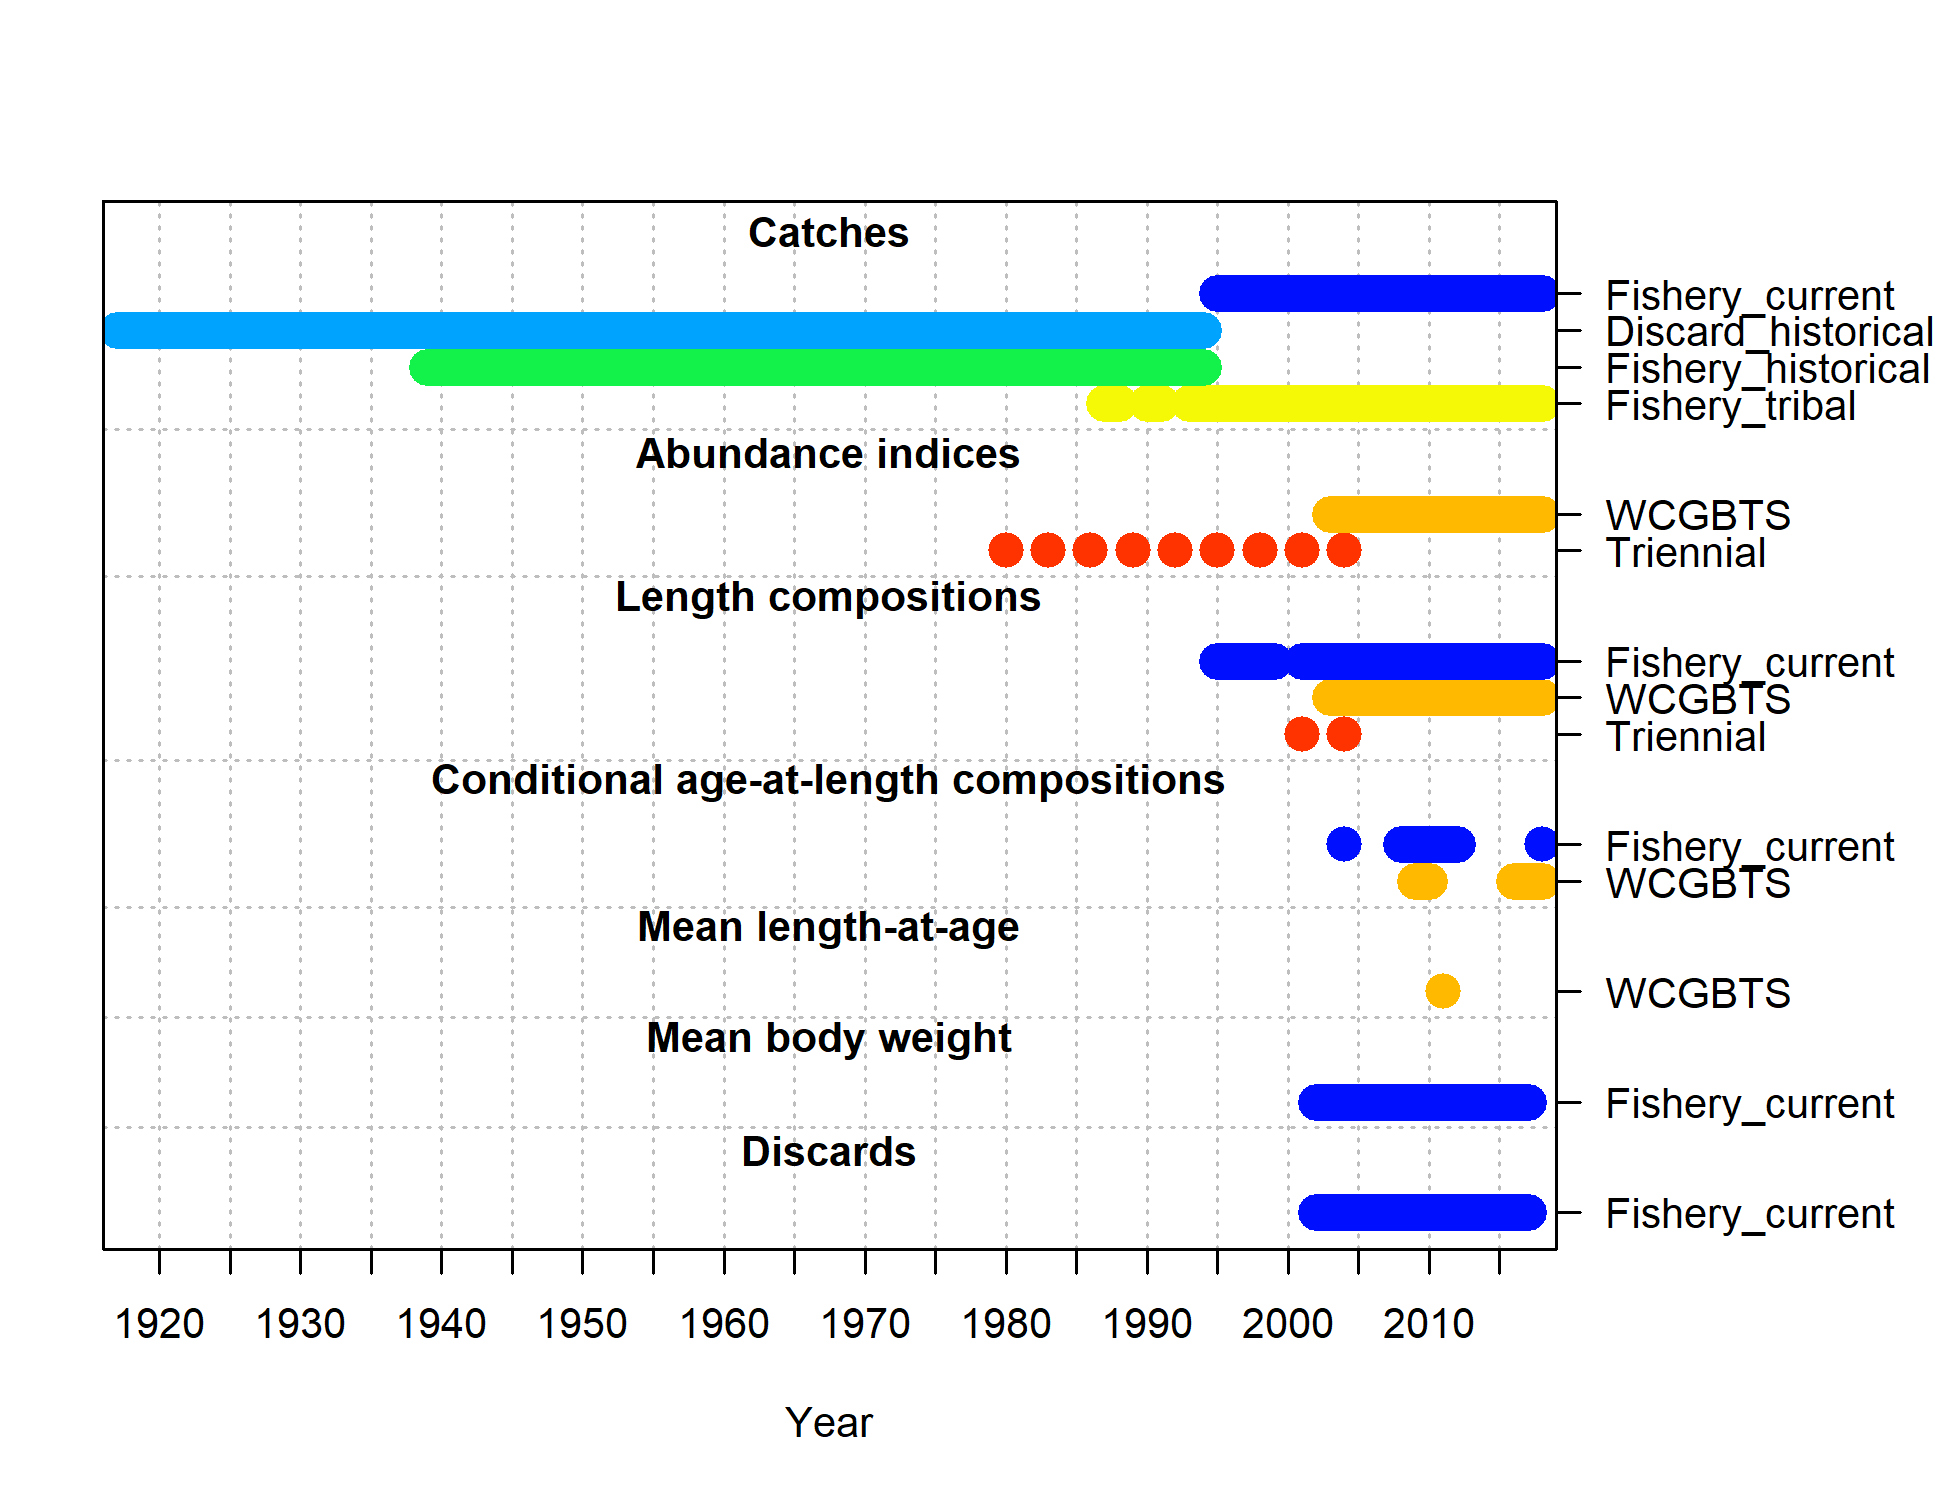
\includegraphics{r4ss/plots_mod1/data_plot.png}
\caption{Summary of data sources used in the model.
\label{fig:data_plot}}
\end{figure}

\FloatBarrier

\FloatBarrier

\FloatBarrier

\FloatBarrier

\FloatBarrier

\FloatBarrier

\FloatBarrier

\newpage

\begin{figure}
\centering
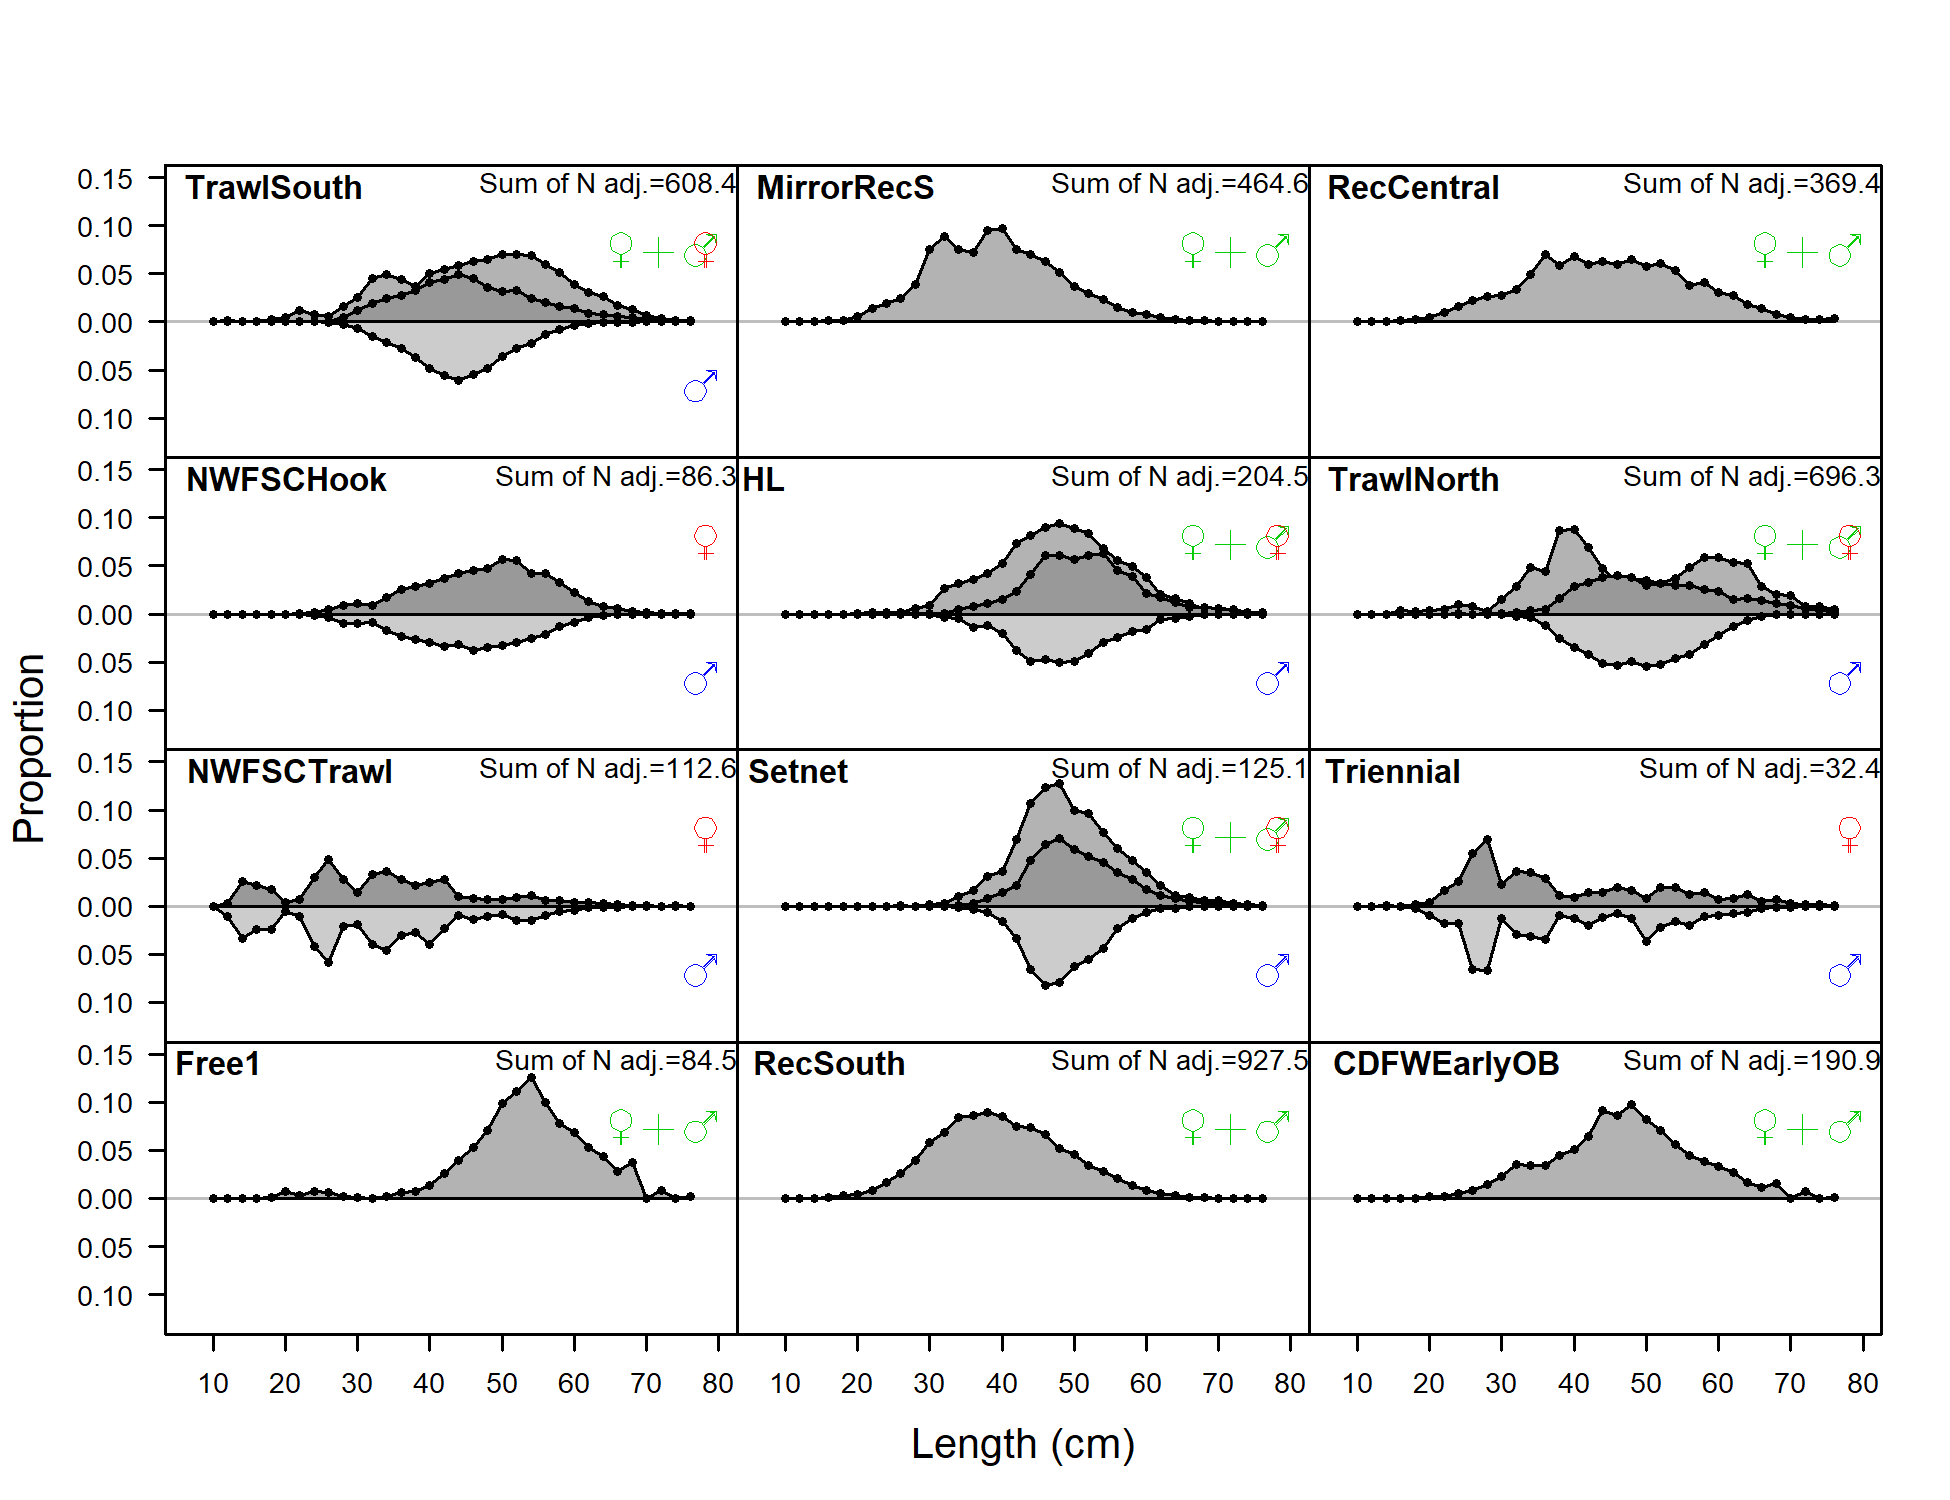
\includegraphics{r4ss/plots_mod1/comp_lendat__aggregated_across_time.png}
\caption{Length comp data, aggregated across time by fleet. Labels
`retained' and `discard' indicate discarded or retained sampled for each
fleet. Panels without this designation represent the whole catch.
\label{fig:comp_lendat_aggregated_across_time}}
\end{figure}

\newpage

\FloatBarrier

\FloatBarrier

\FloatBarrier

\FloatBarrier

\begin{figure}
\centering
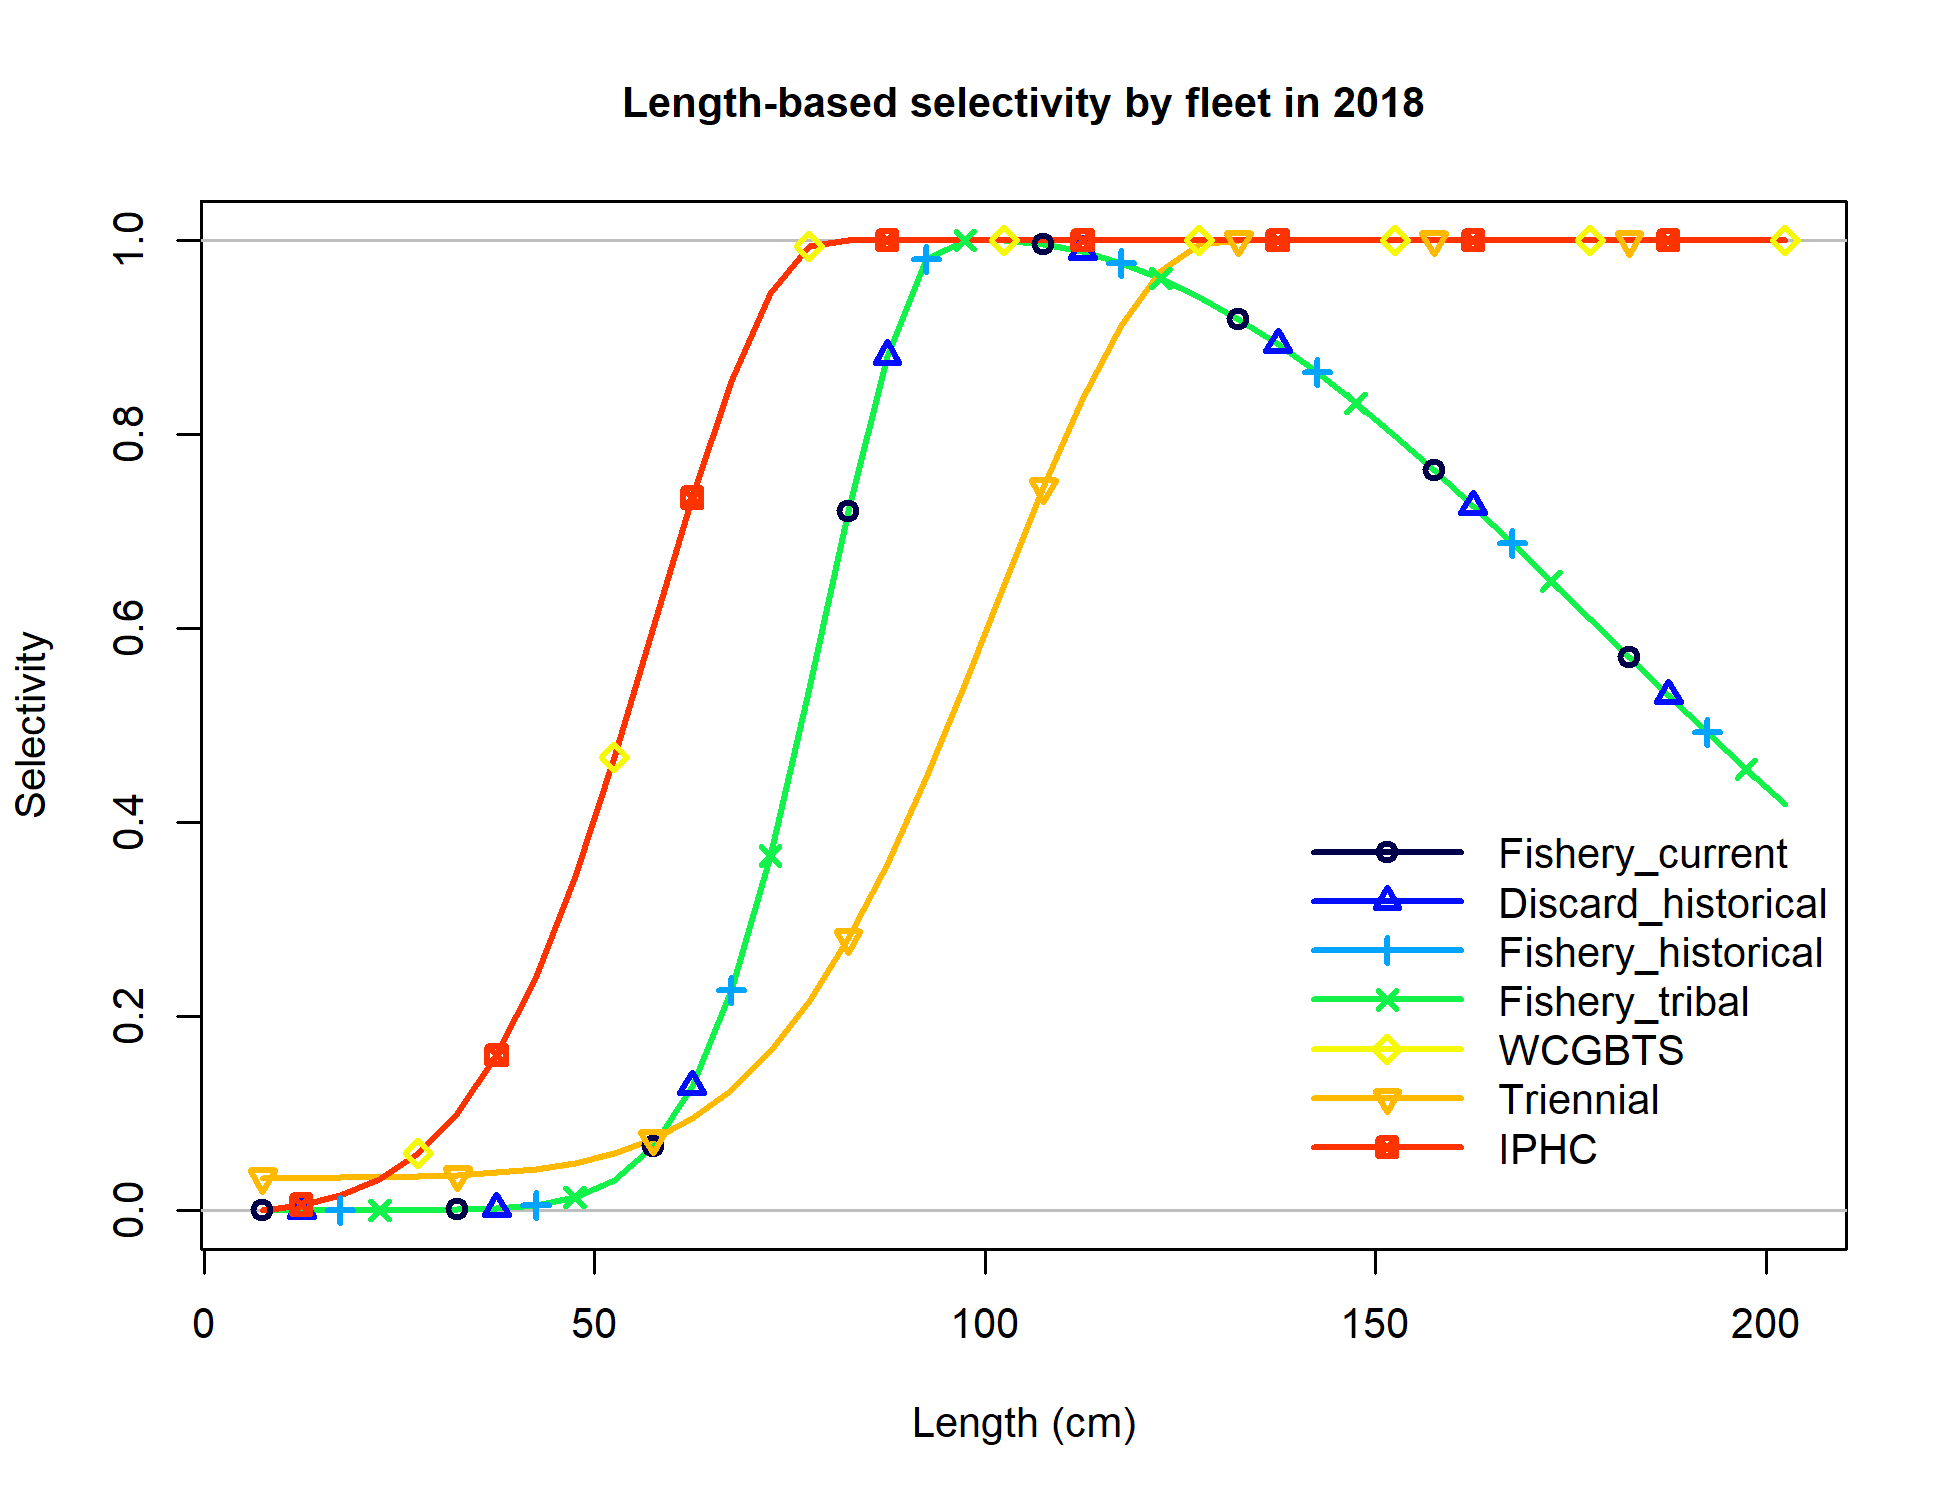
\includegraphics{r4ss/plots_mod1/sel01_multiple_fleets_length1.png}
\caption{Selectivity at length for all of the fleets in the base model.
\label{fig:sel01_multiple_fleets_length1}}
\end{figure}

\FloatBarrier

\begin{figure}
\centering
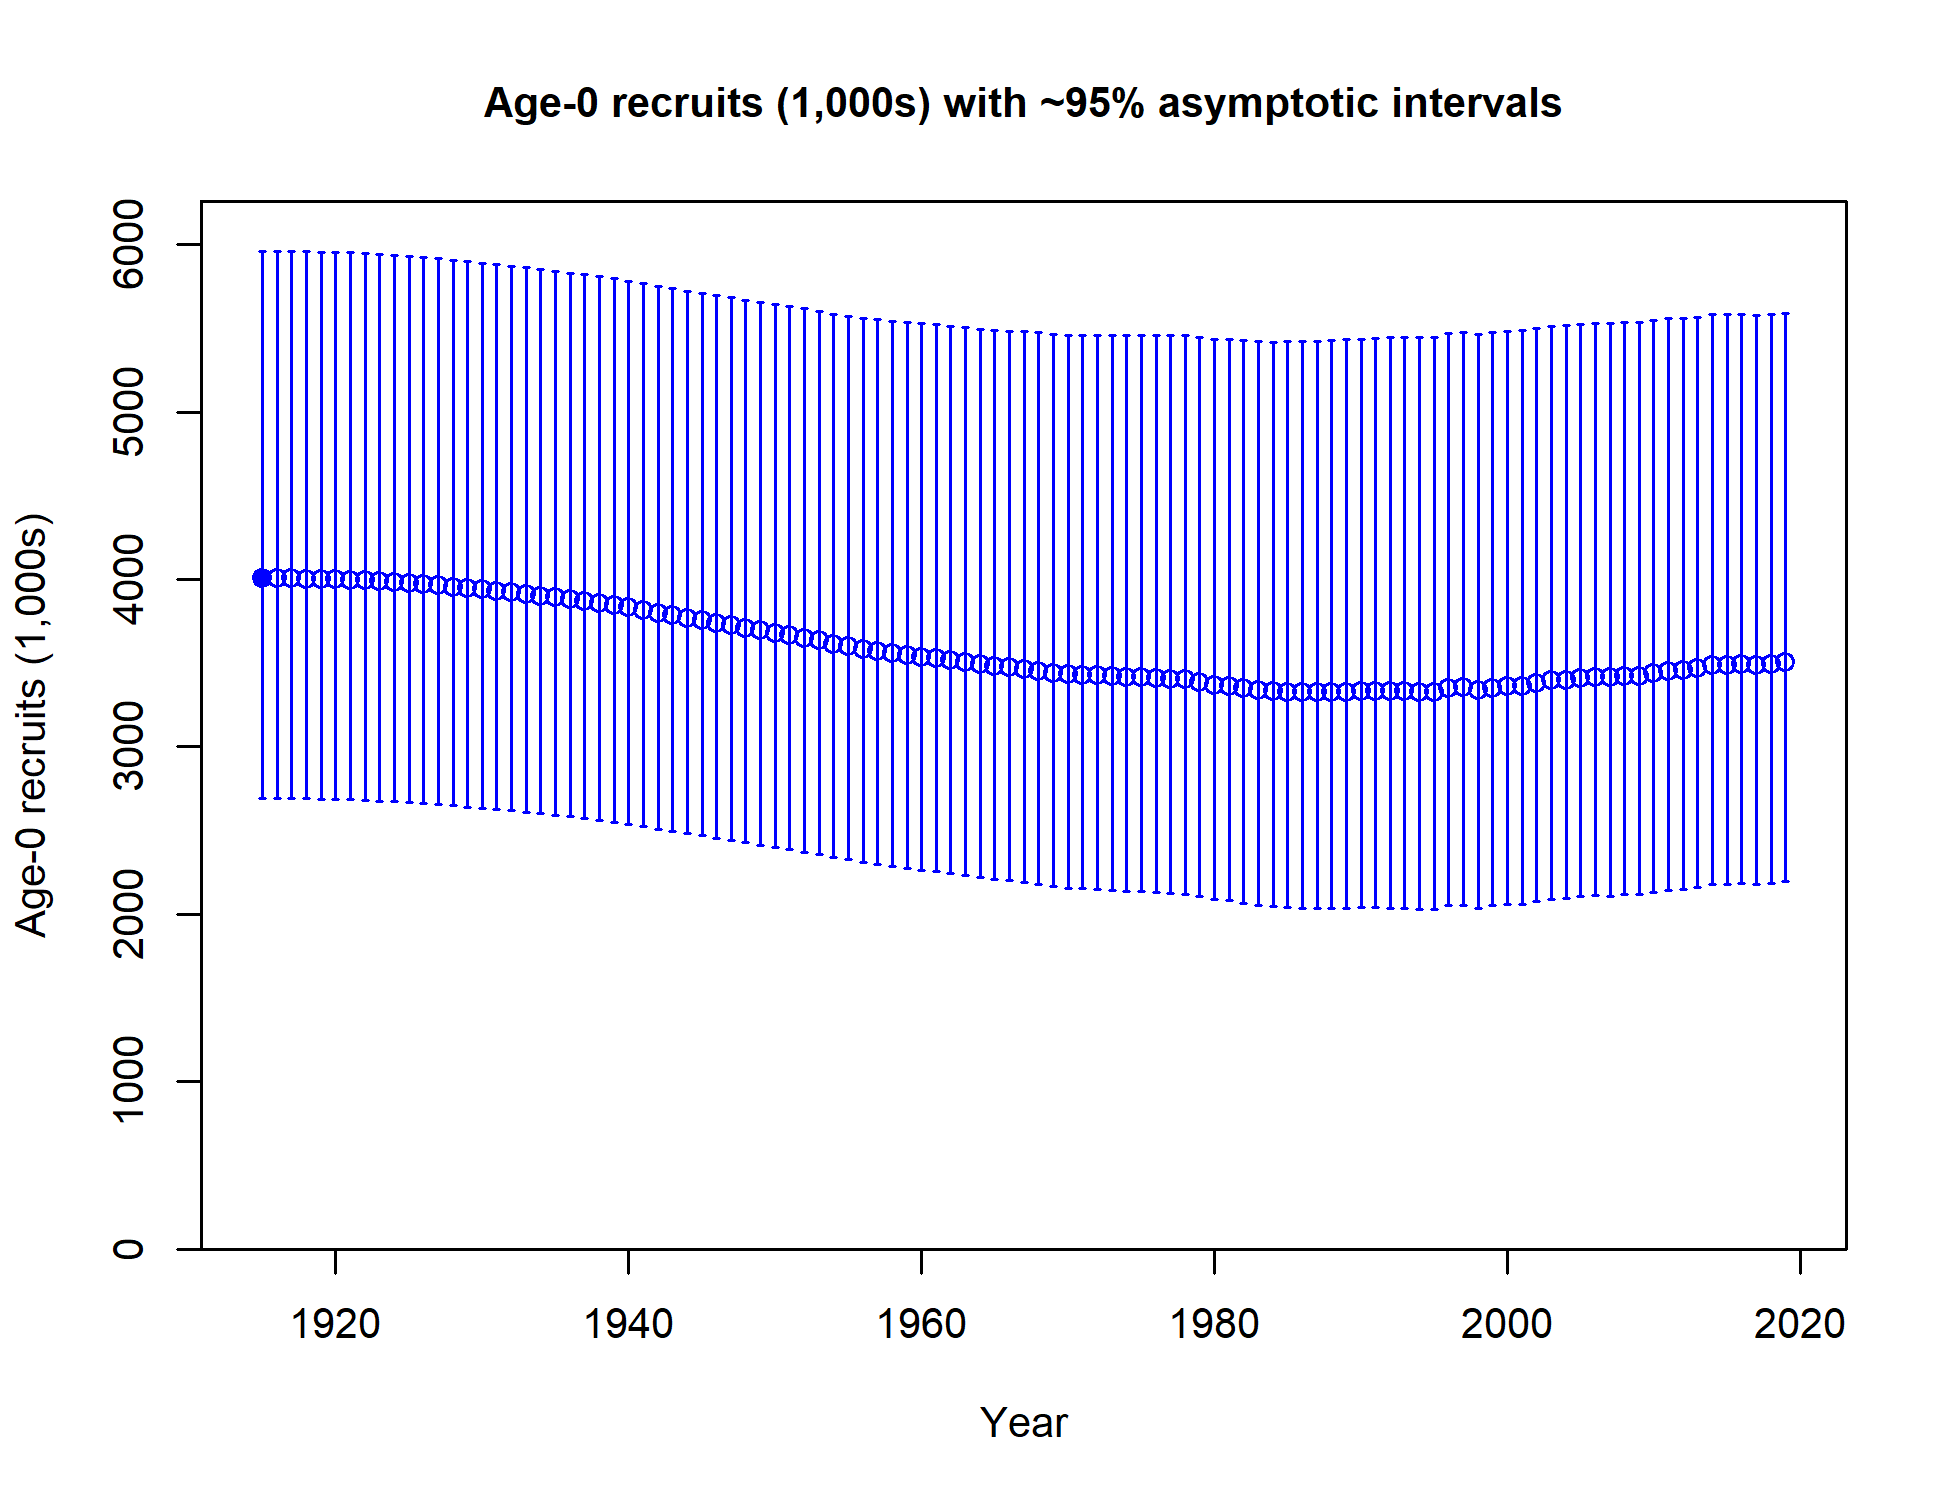
\includegraphics{r4ss/plots_mod1/ts11_Age-0_recruits_(1000s)_with_95_asymptotic_intervals.png}
\caption{Estimated time-series of recruitment for Big Skate.
\label{fig:ts11_Age-0_recruits_(1000s)_with_95_asymptotic_intervals}}
\end{figure}

\begin{figure}
\centering
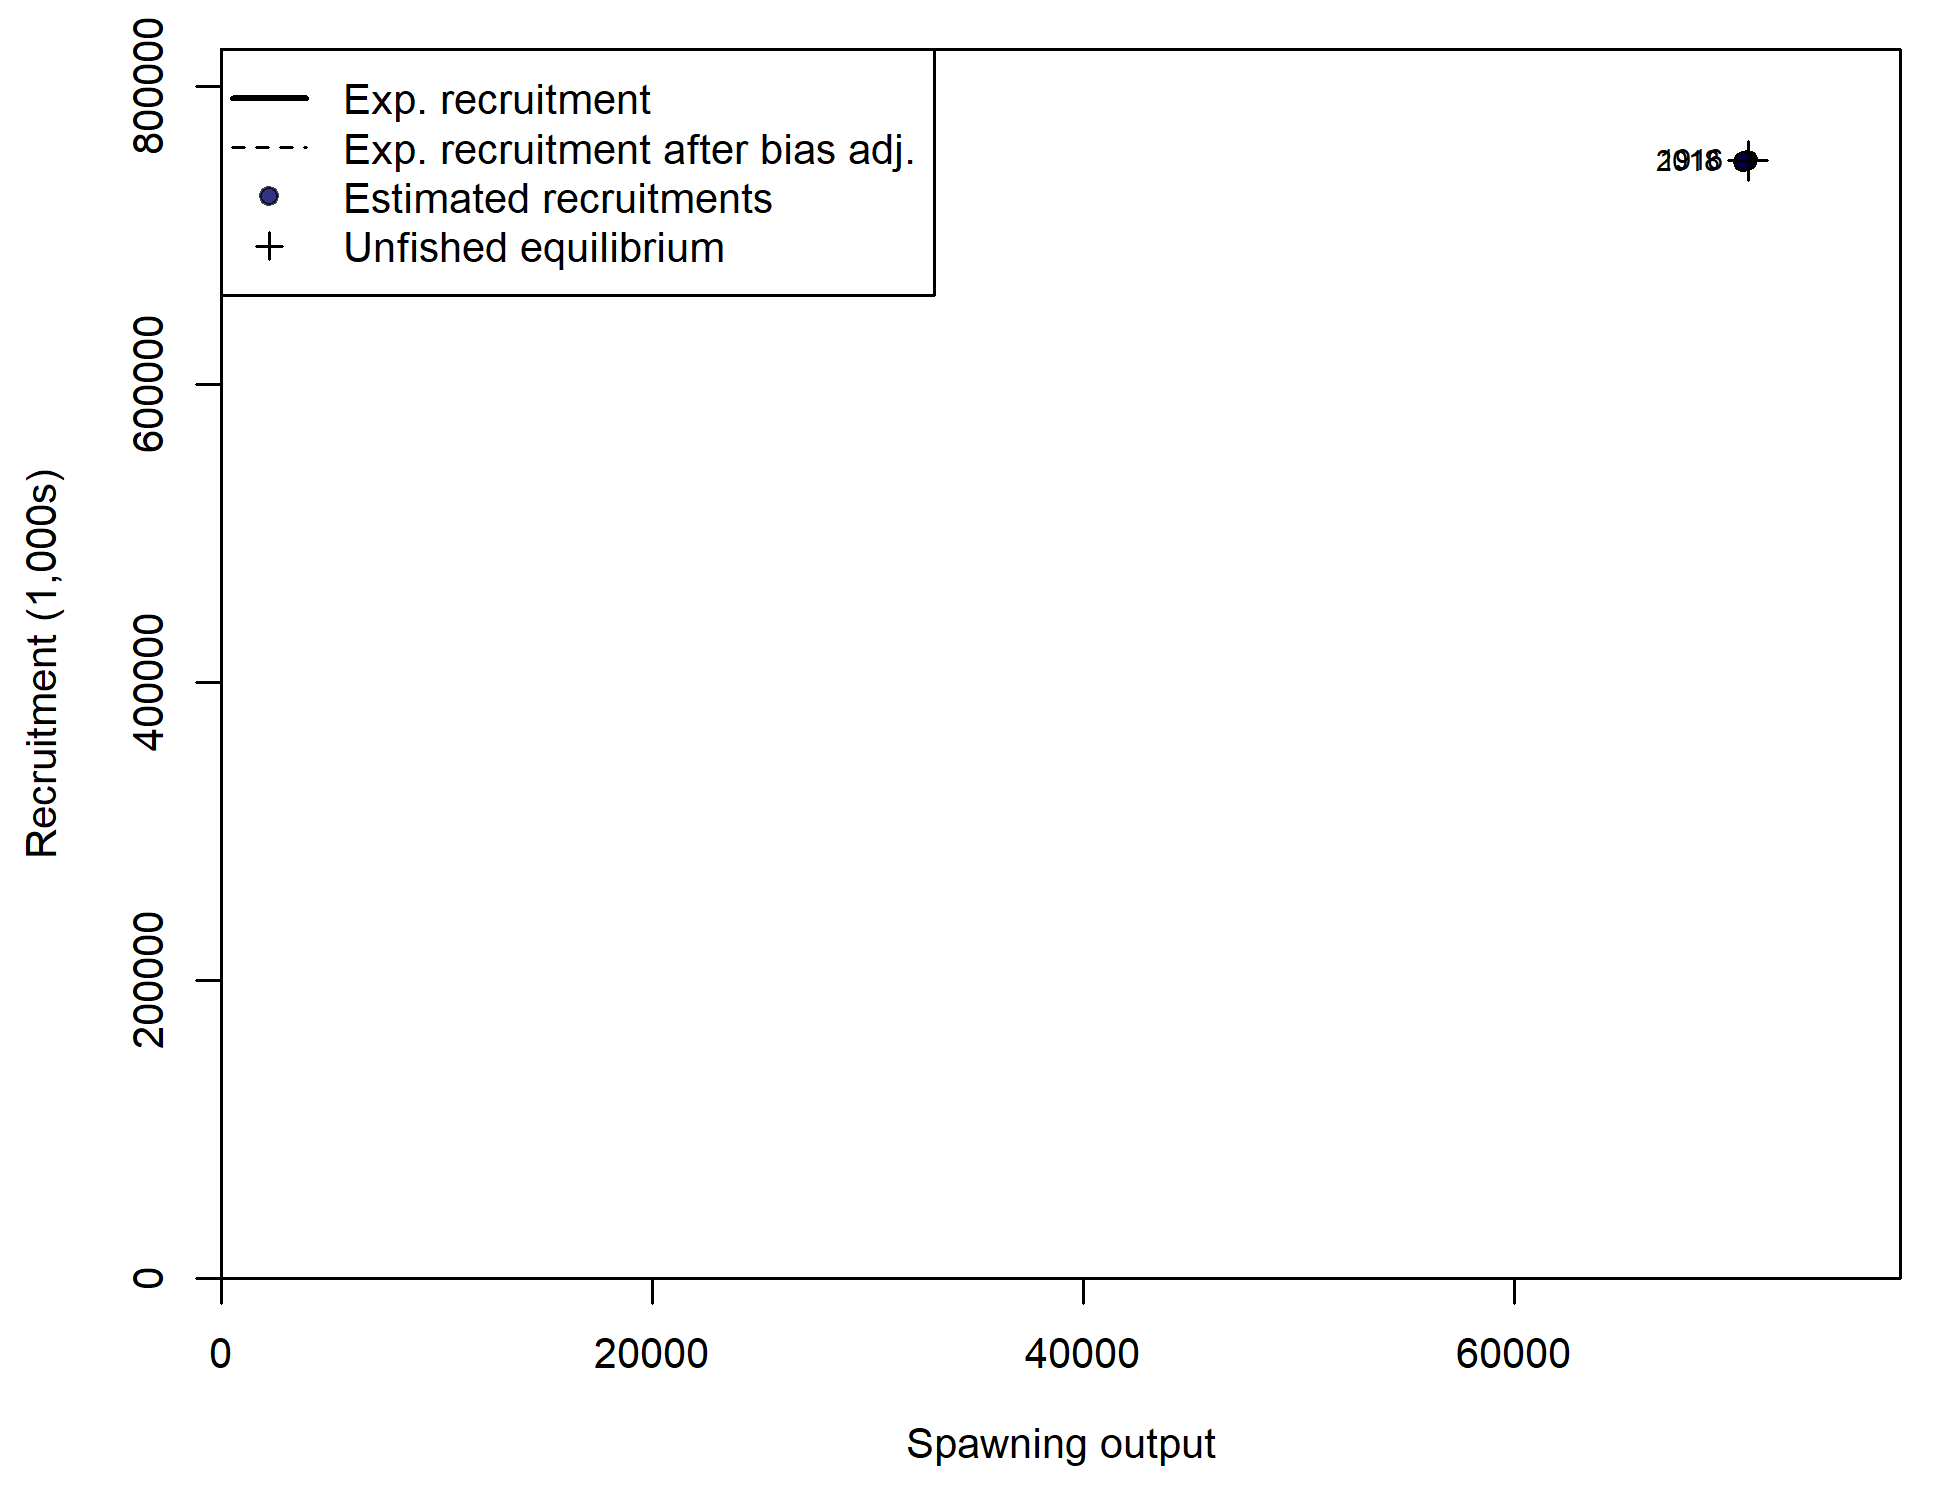
\includegraphics{r4ss/plots_mod1/SR_curve2.png}
\caption{Estimated recruitment (red circles) and the assumed
stock-recruit relationship (black line) for Big Skate. The green line
shows the effect of the bias correction for the lognormal distribution.
\label{fig:SR_curve2}}
\end{figure}

\FloatBarrier

\begin{figure}
\centering
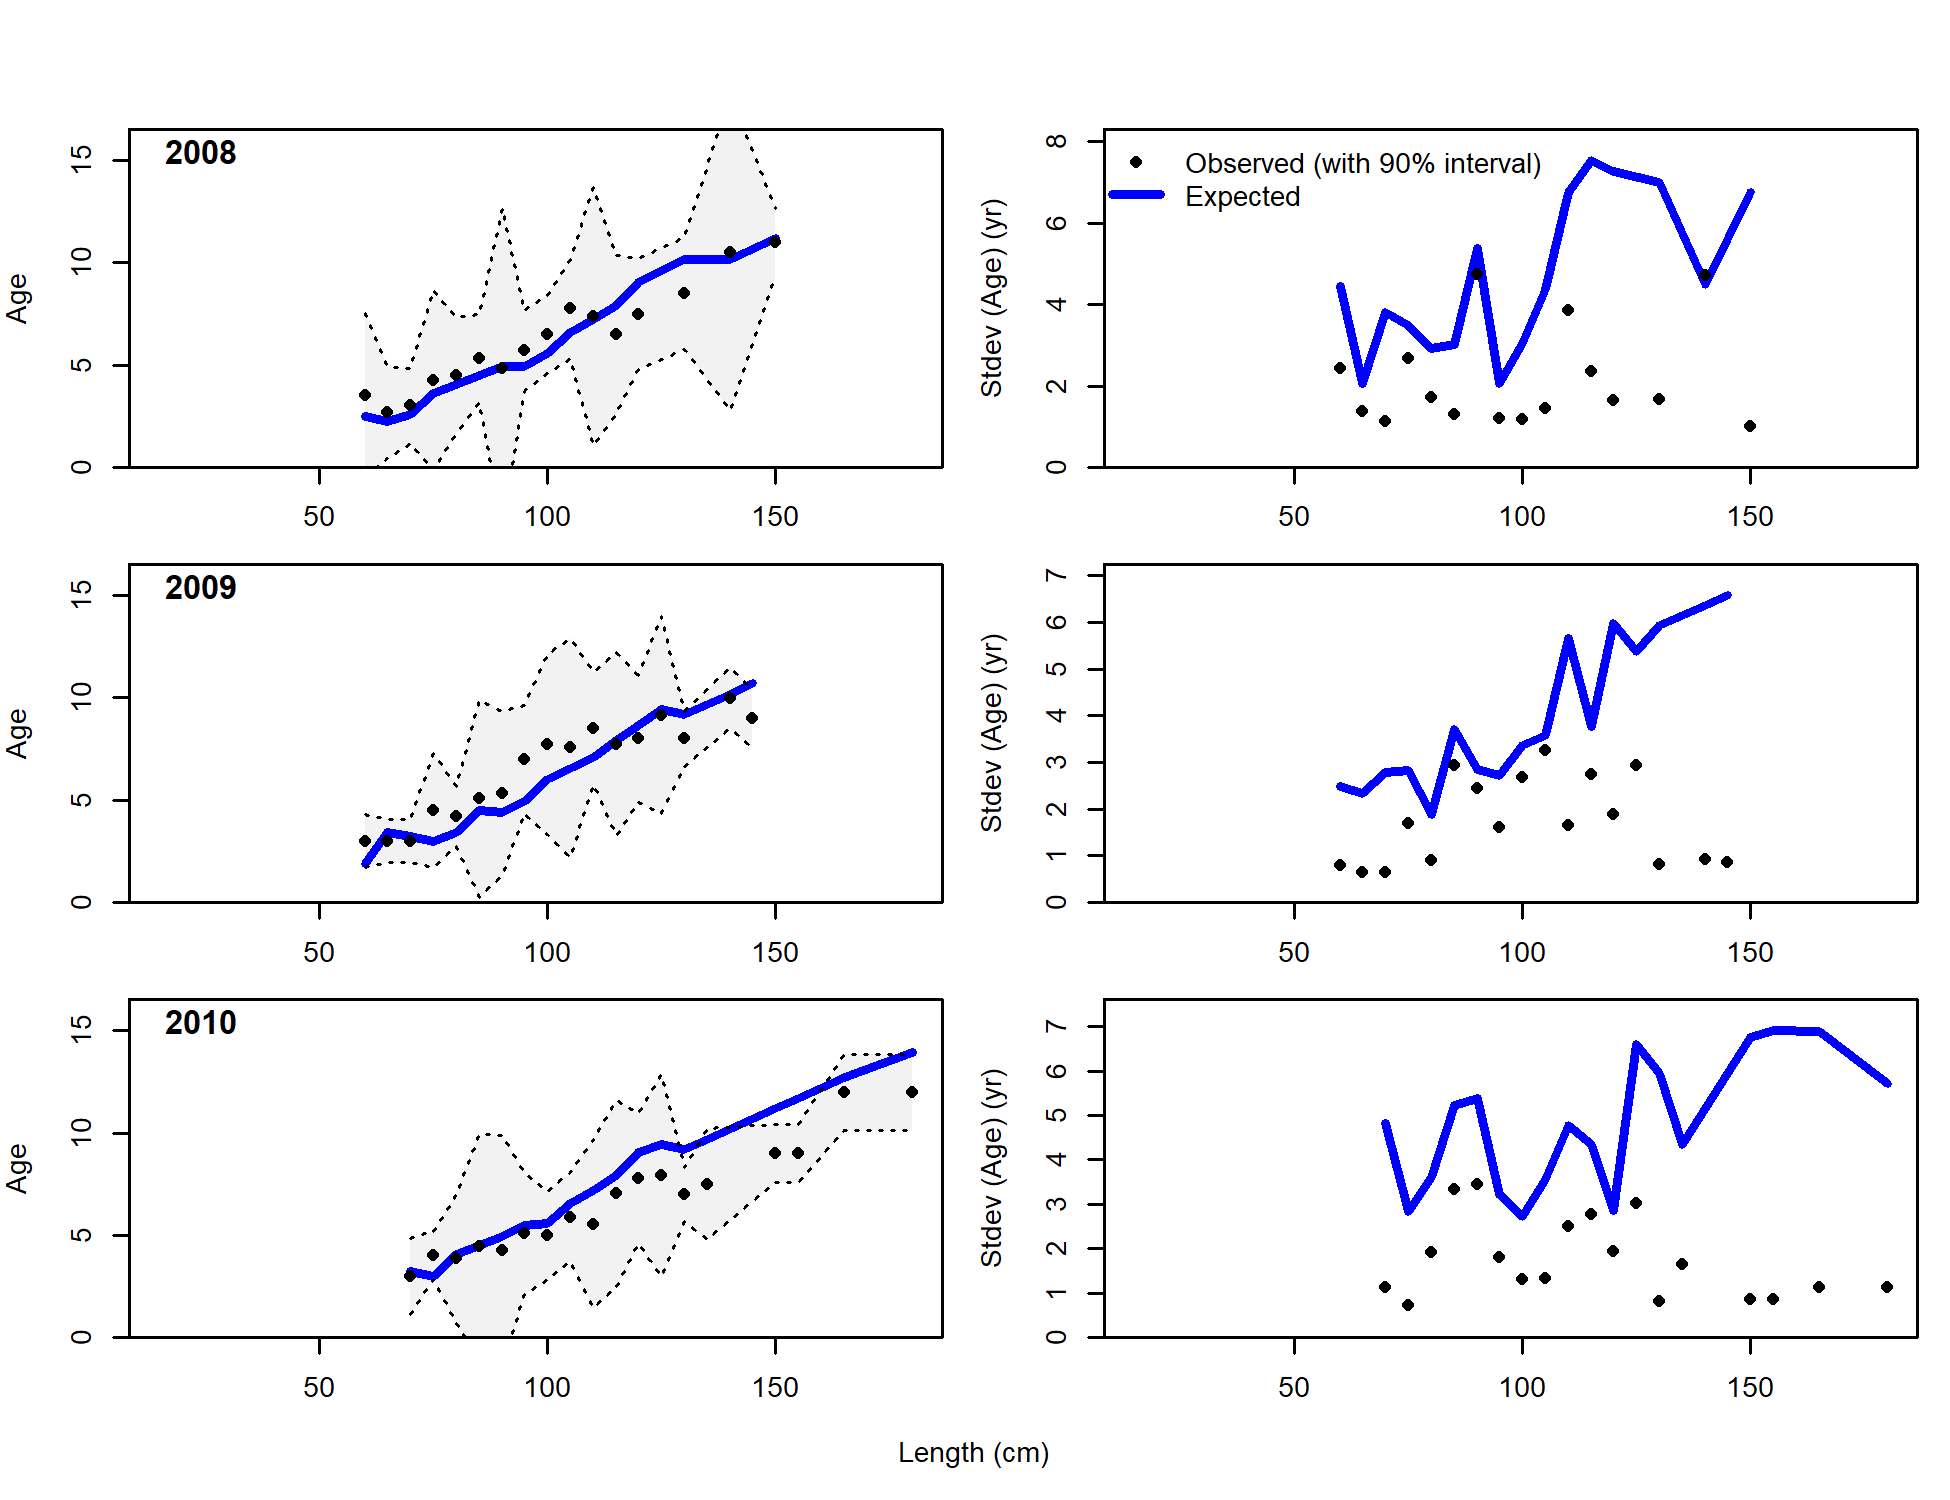
\includegraphics{./r4ss/plots_mod1/comp_condAALfit_Andre_plotsflt1mkt2_page1.png}
\caption{Conditional AAL plot, retained, Fishery\_current (plot 1 of 2)
These plots show mean age and std. dev. in conditional AAL. Left plots
are mean AAL by size\_class (obs. and pred.) with 90\% CIs based on
adding 1.64 SE of mean to the data. Right plots in each pair are SE of
mean AAL (obs. and pred.) with 90\% CIs based on the chi\_square
distribution.
\label{fig:mod1_4_comp_condAALfit_Andre_plotsflt1mkt2_page1}}
\end{figure}

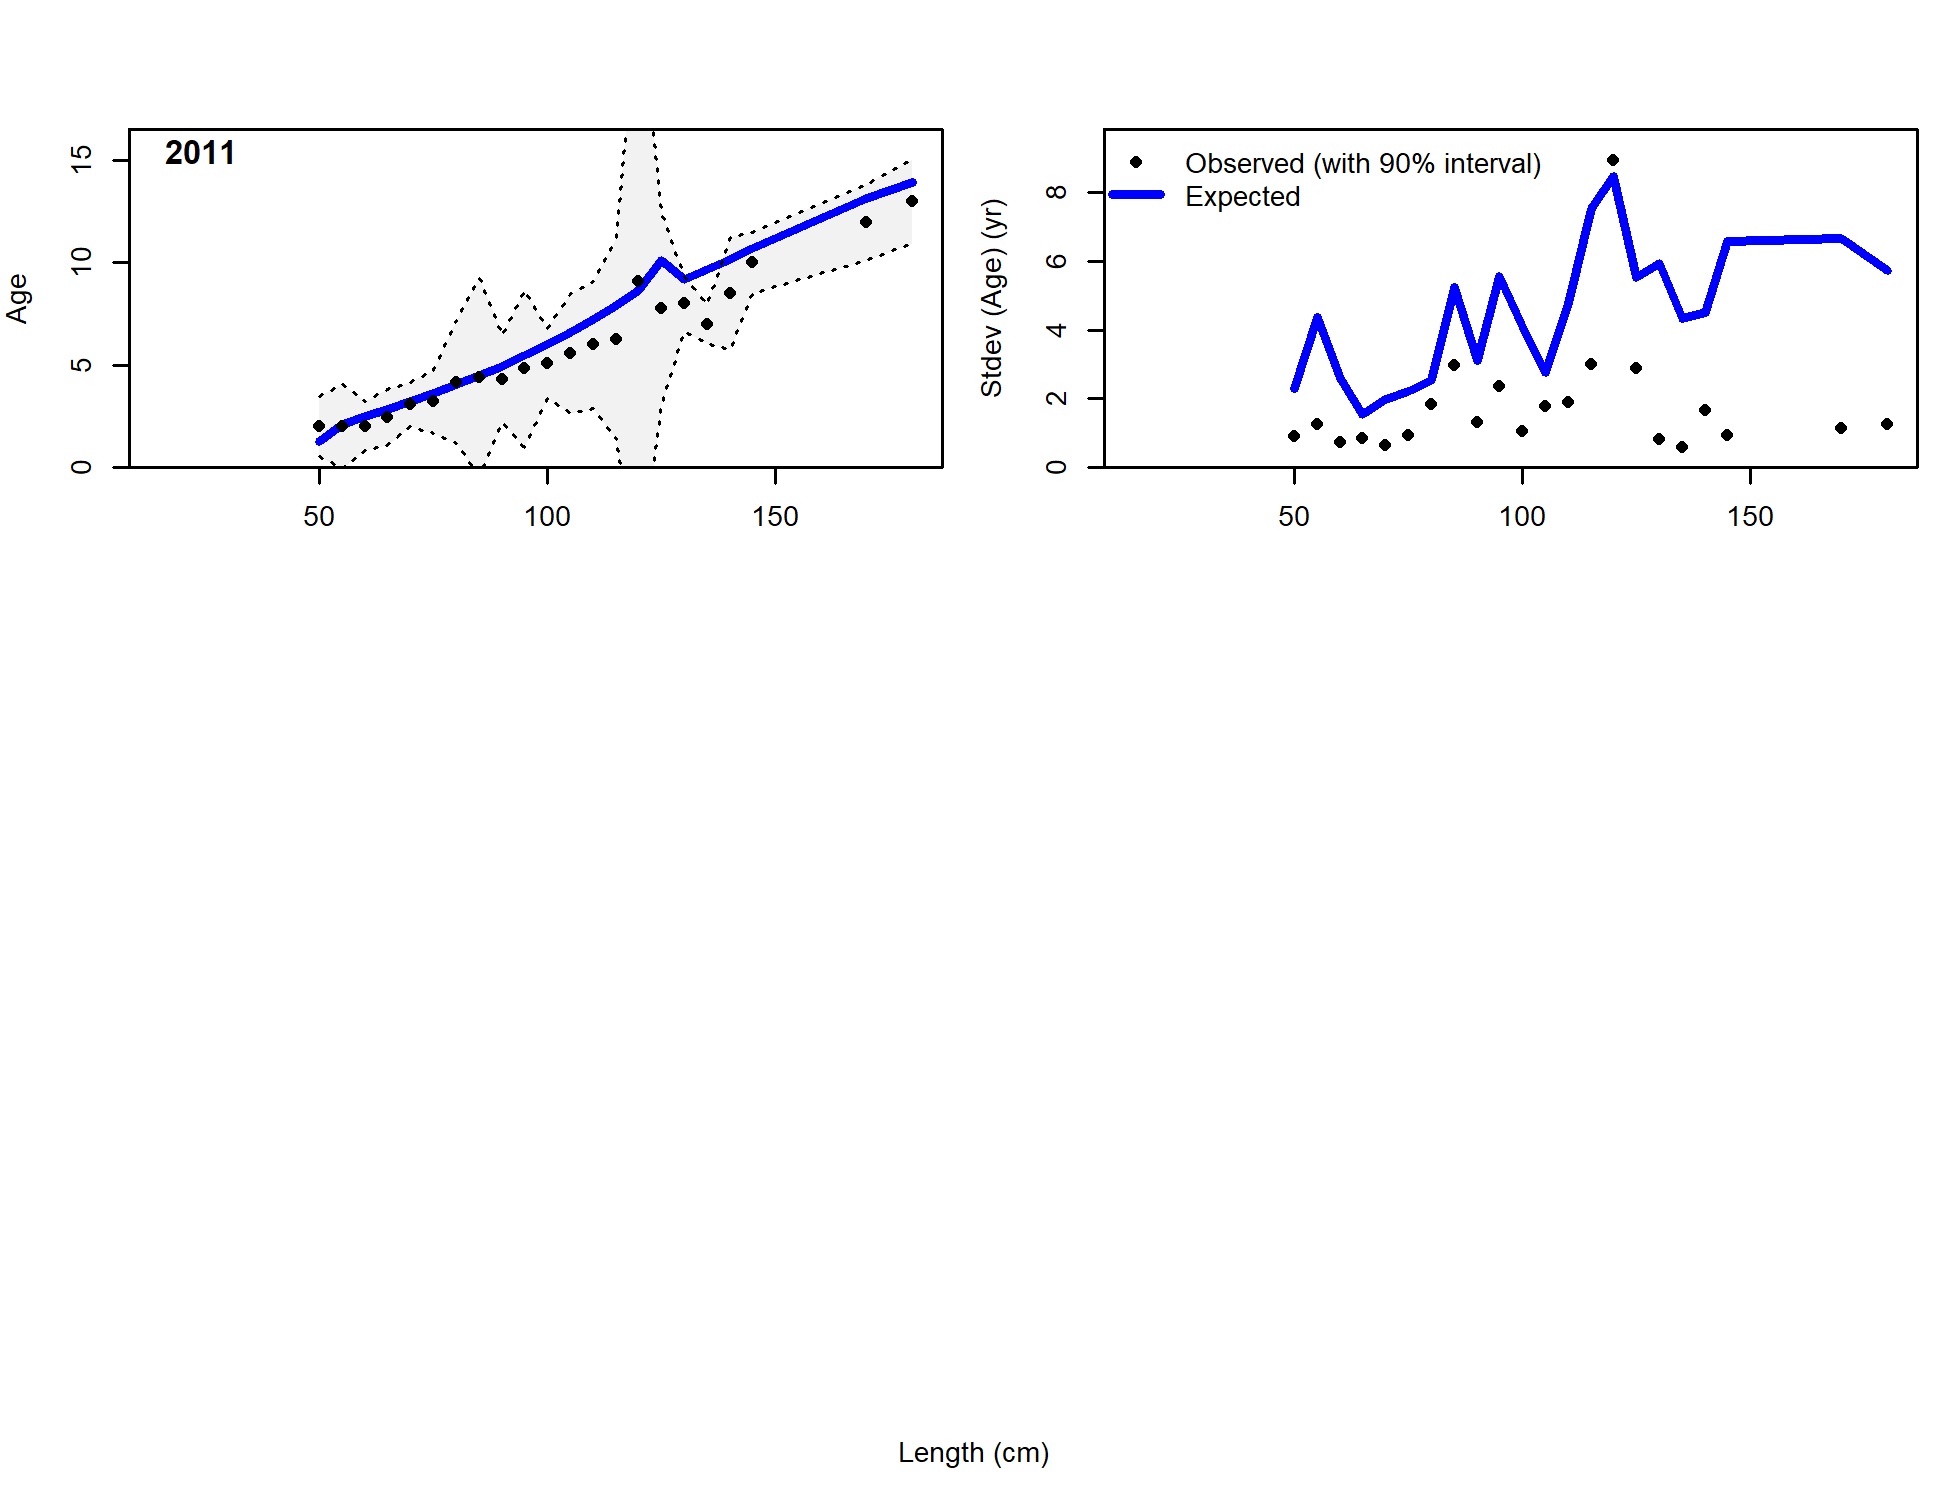
\includegraphics{./r4ss/plots_mod1/comp_condAALfit_Andre_plotsflt1mkt2_page2.png}

\begin{center} 

              Figure continued from previous page 

             \end{center}

\begin{figure}
\centering
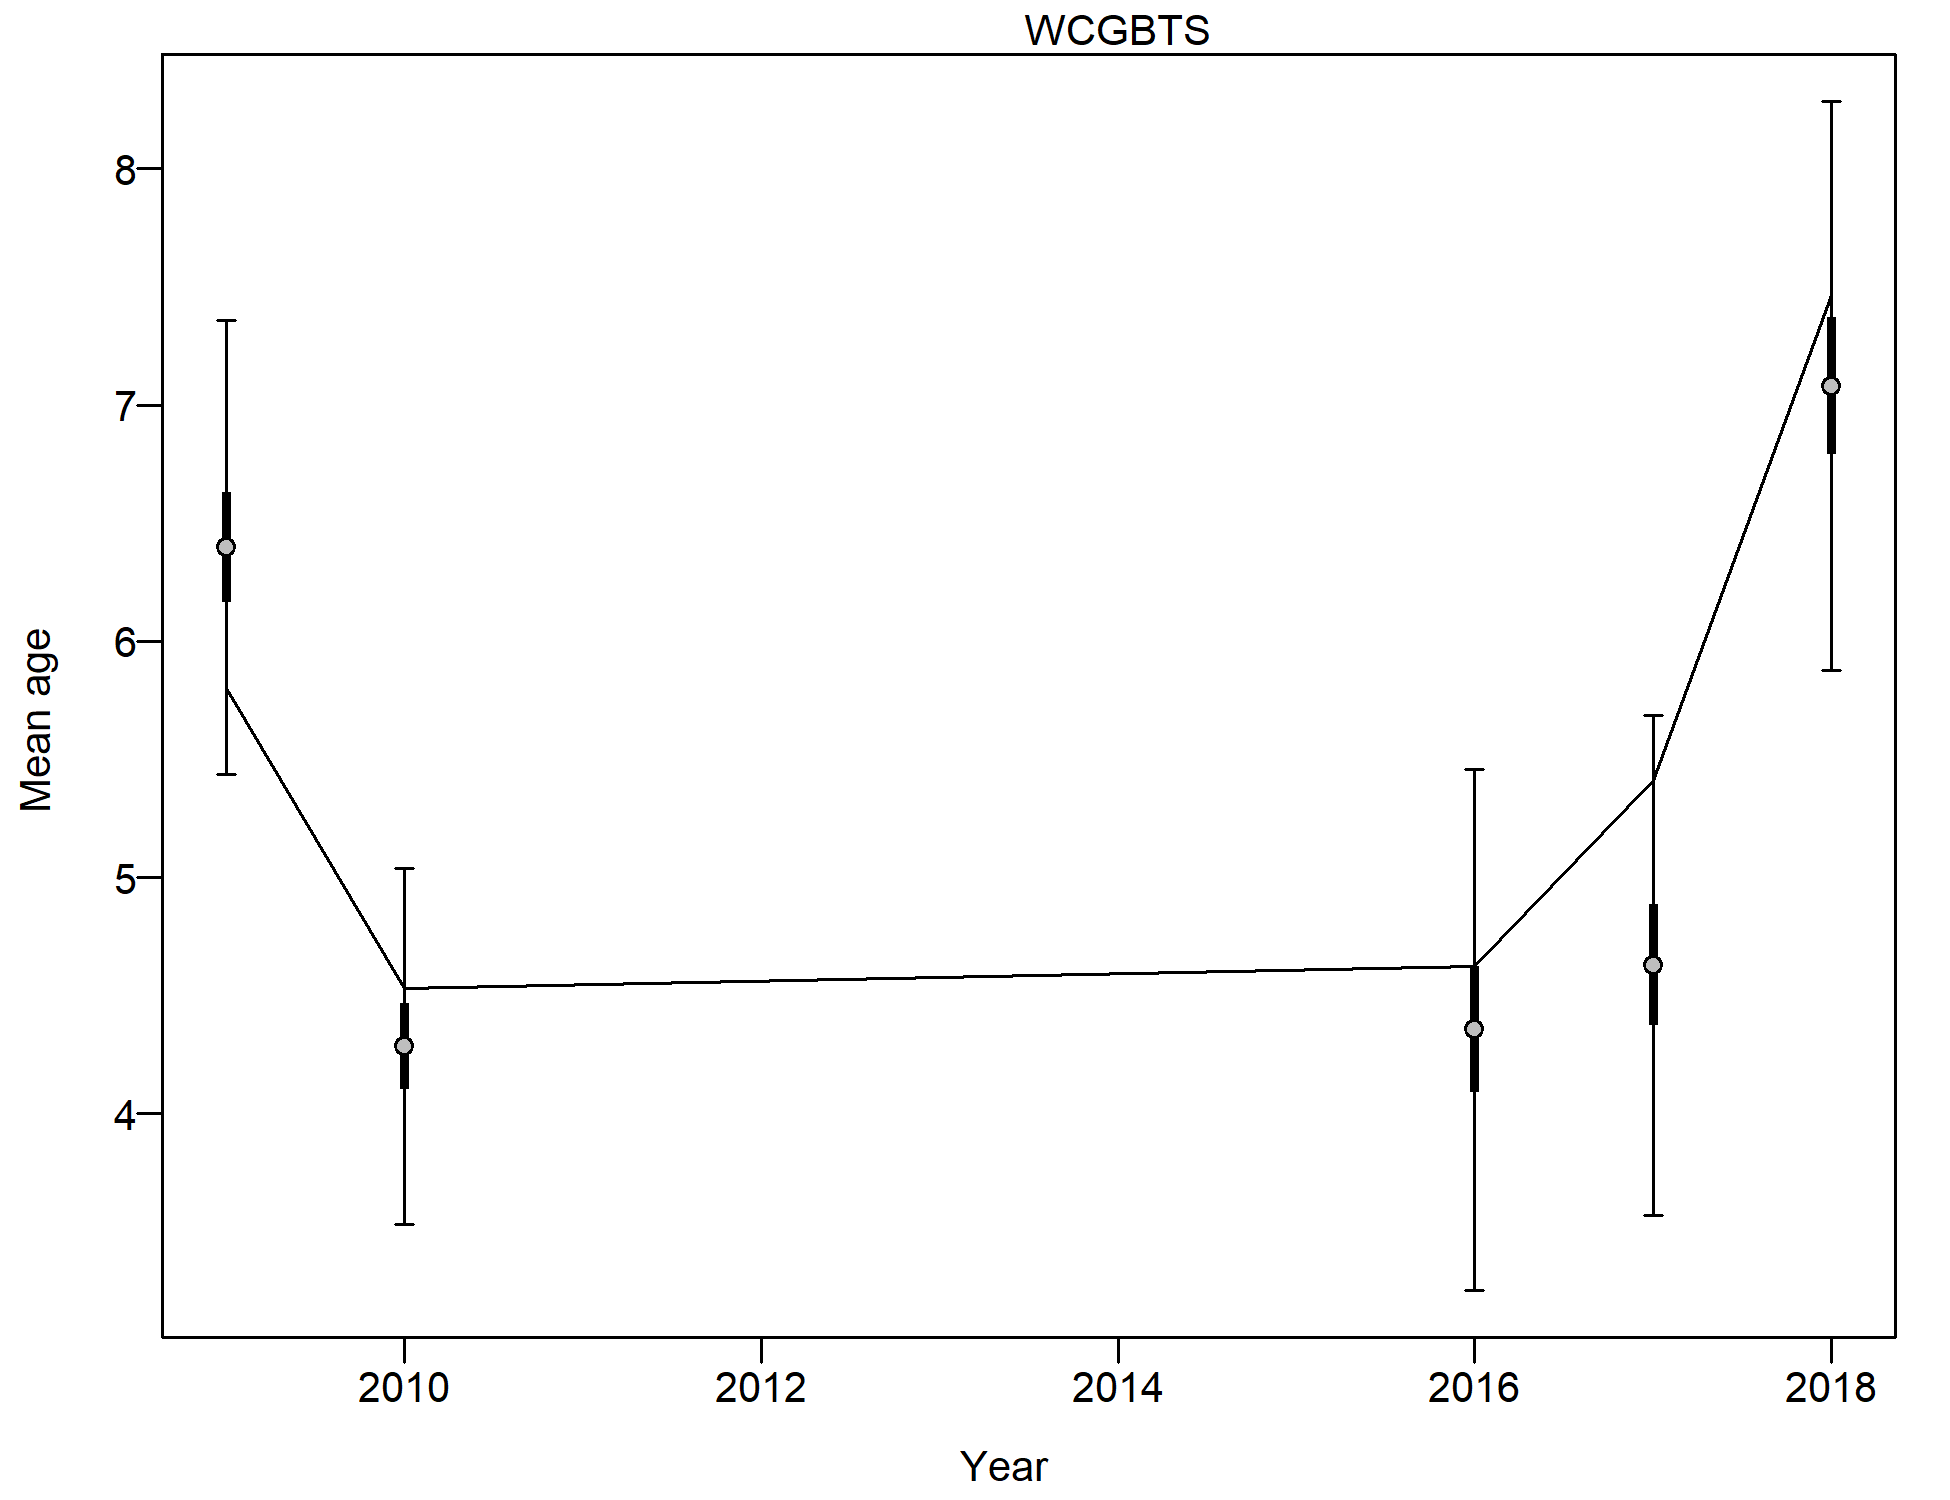
\includegraphics{./r4ss/plots_mod1/comp_condAALfit_data_weighting_TA1.8_condAgeWCGBTS.png}
\caption{Mean age from conditional data (aggregated across length bins)
for WCGBTS with 95\% confidence intervals based on current samples
sizes. Francis data weighting method TA1.8: thinner intervals (with
capped ends) show result of further adjusting sample sizes based on
suggested multiplier (with 95\% interval) for conditional
age\_at\_length data from WCGBTS: 1.3806 (0.8289\_39.92) For more info,
see Francis, R.I.C.C. (2011). Data weighting in statistical fisheries
stock assessment models. Can. J. Fish. Aquat. Sci. 68: 1124\_1138.
\label{fig:mod1_6_comp_condAALfit_data_weighting_TA1.8_condAgeWCGBTS}}
\end{figure}

\begin{figure}
\centering
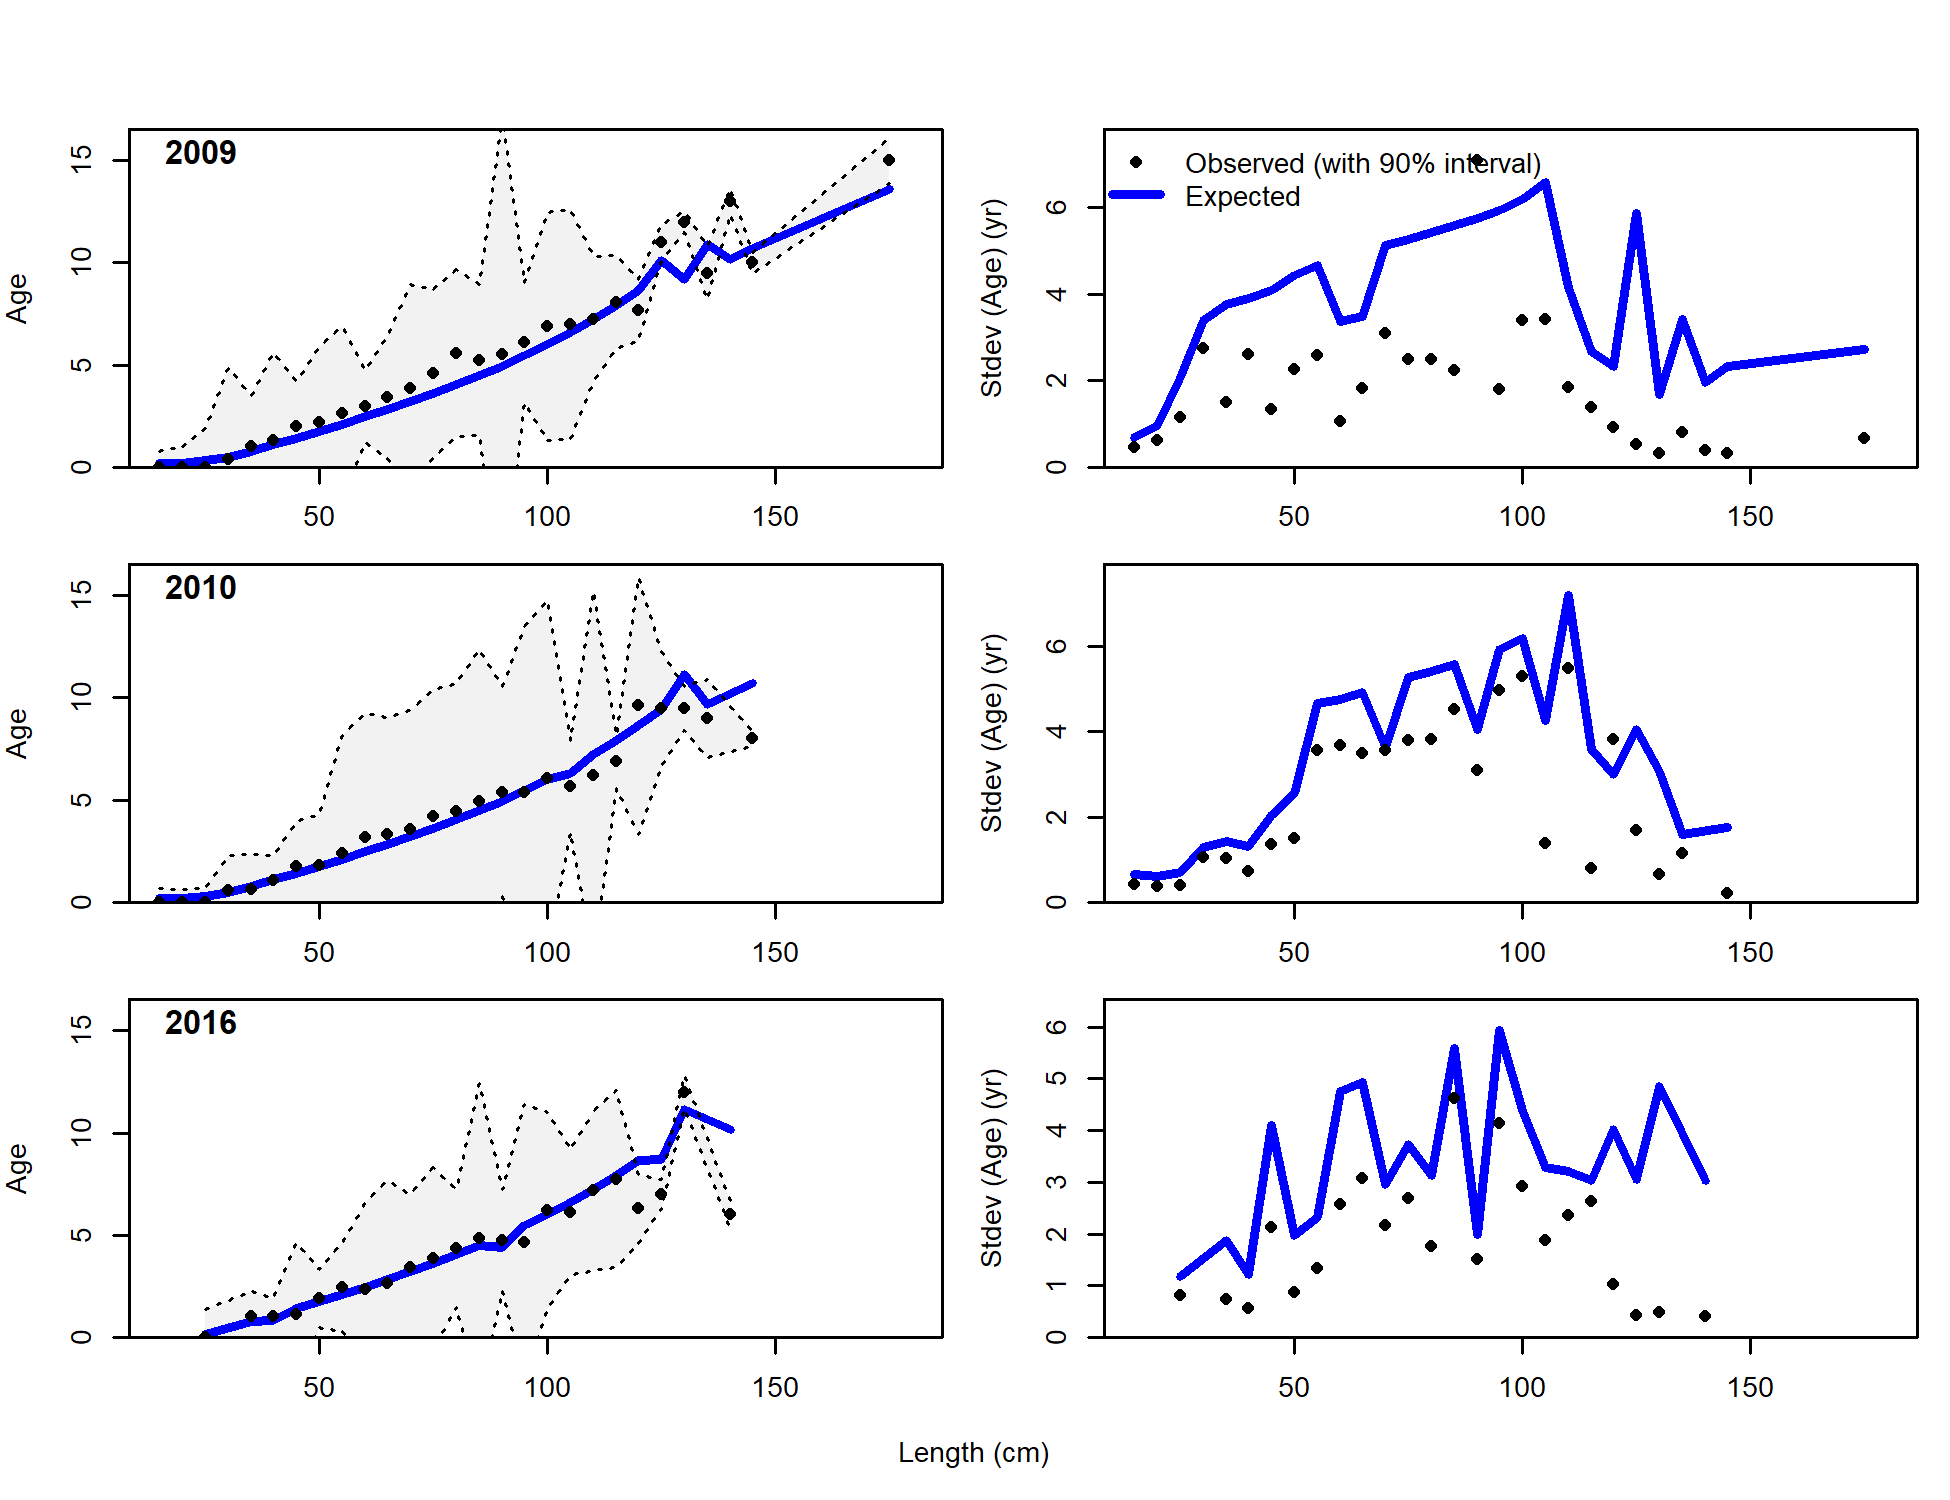
\includegraphics{./r4ss/plots_mod1/comp_condAALfit_Andre_plotsflt5mkt0_page1.png}
\caption{Conditional AAL plot, whole catch, WCGBTS (plot 1 of 2) These
plots show mean age and std. dev. in conditional AAL. Left plots are
mean AAL by size\_class (obs. and pred.) with 90\% CIs based on adding
1.64 SE of mean to the data. Right plots in each pair are SE of mean AAL
(obs. and pred.) with 90\% CIs based on the chi\_square distribution.
\label{fig:mod1_7_comp_condAALfit_Andre_plotsflt5mkt0_page1}}
\end{figure}

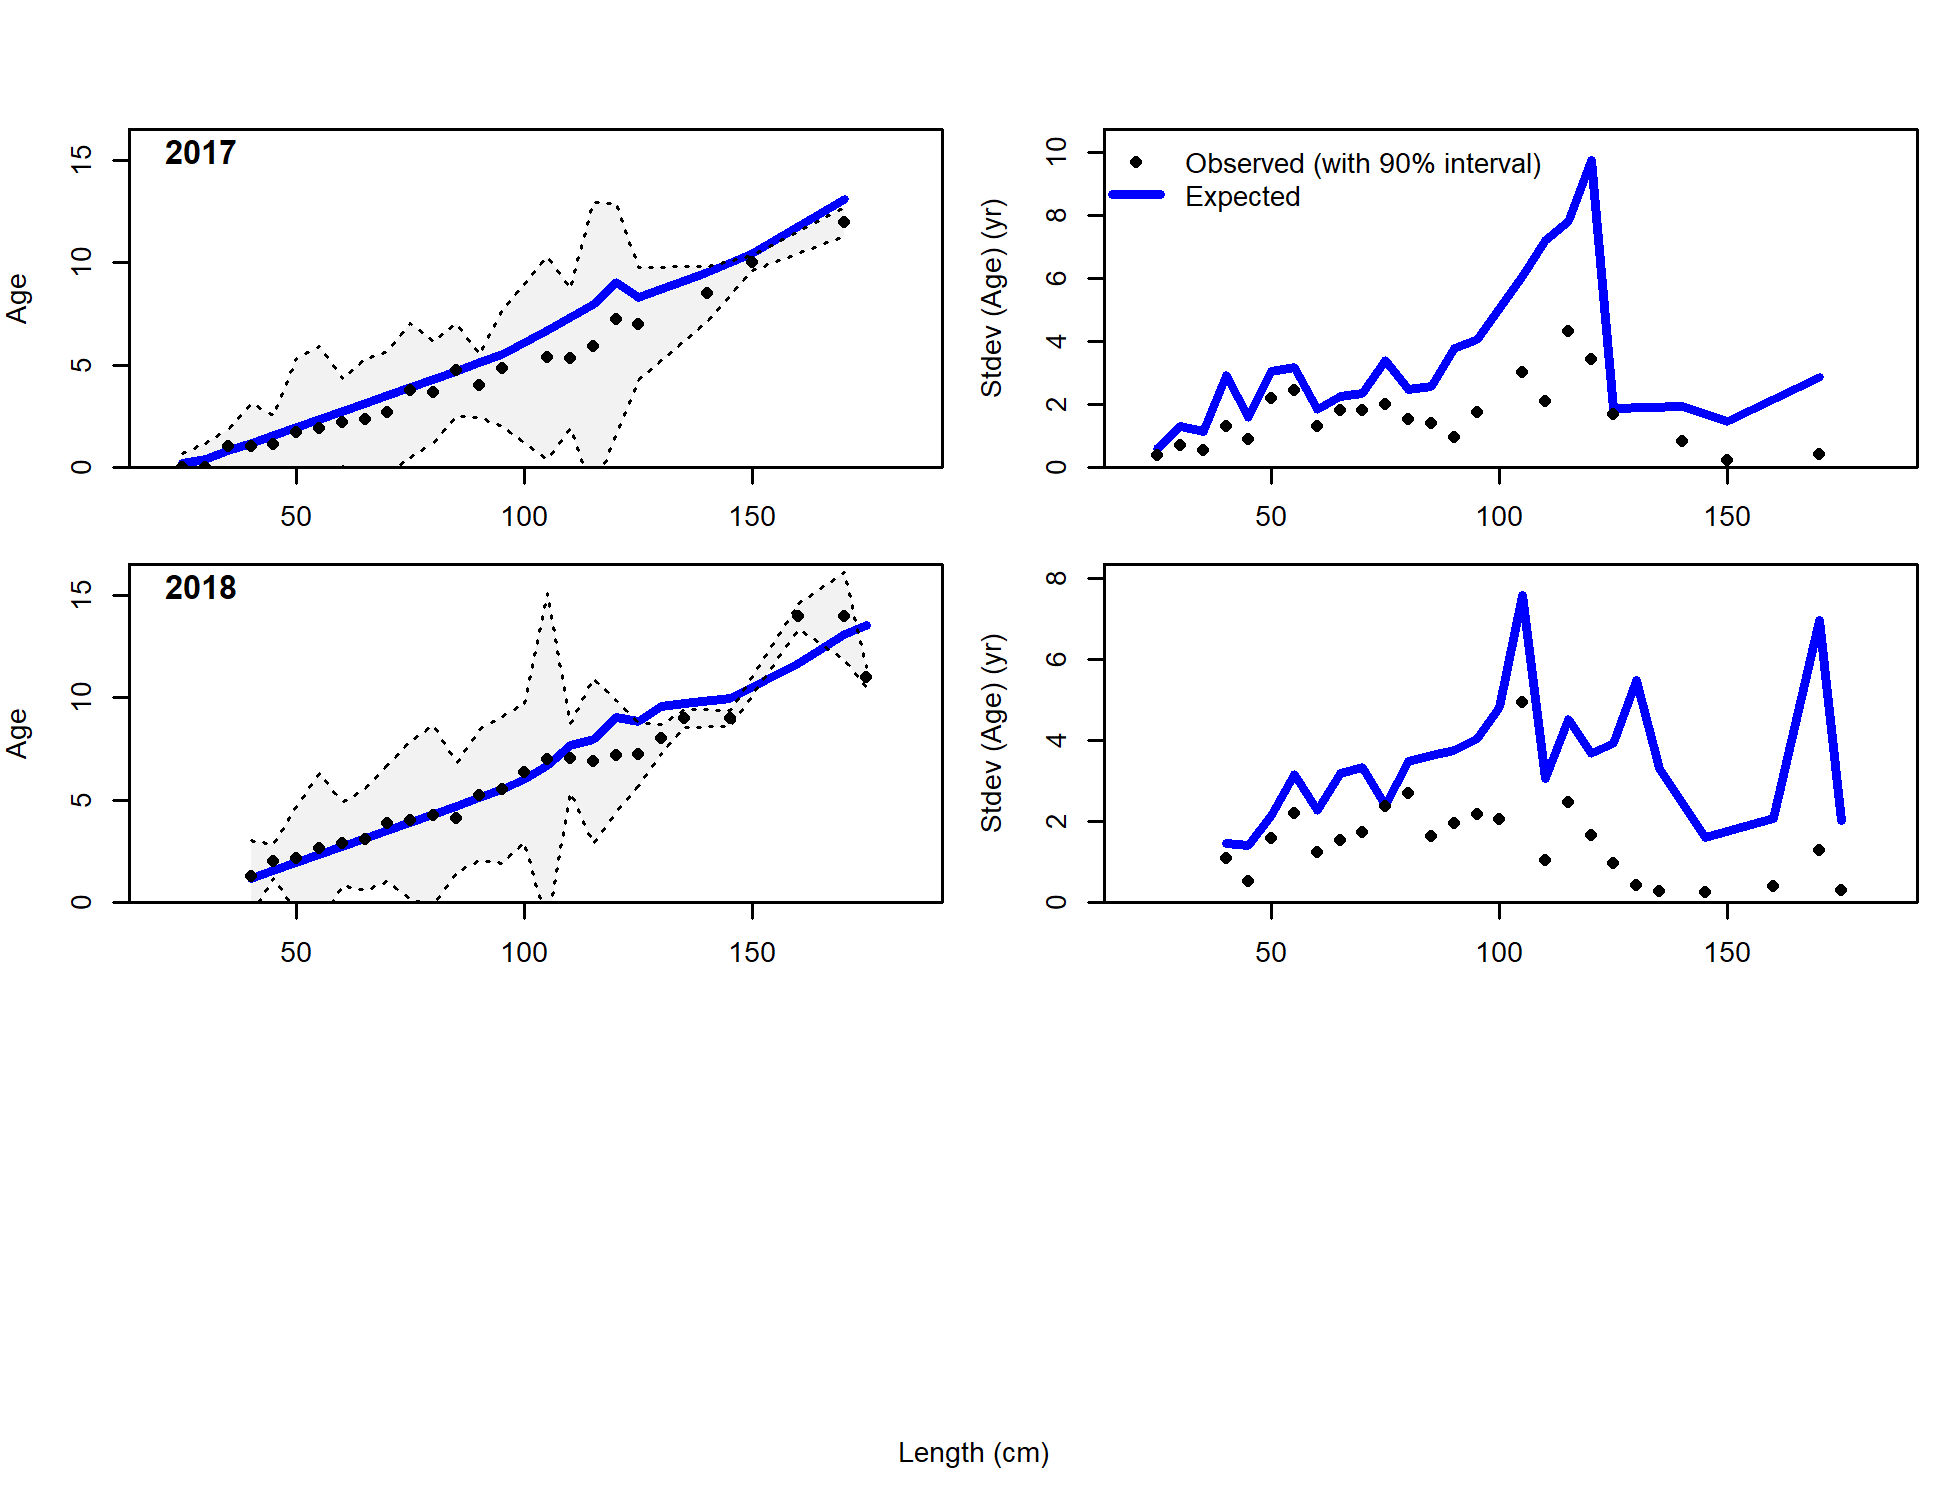
\includegraphics{./r4ss/plots_mod1/comp_condAALfit_Andre_plotsflt5mkt0_page2.png}

\begin{center} 

              Figure continued from previous page 

             \end{center}

\FloatBarrier

\FloatBarrier

\FloatBarrier

\FloatBarrier

\begin{figure}
\centering
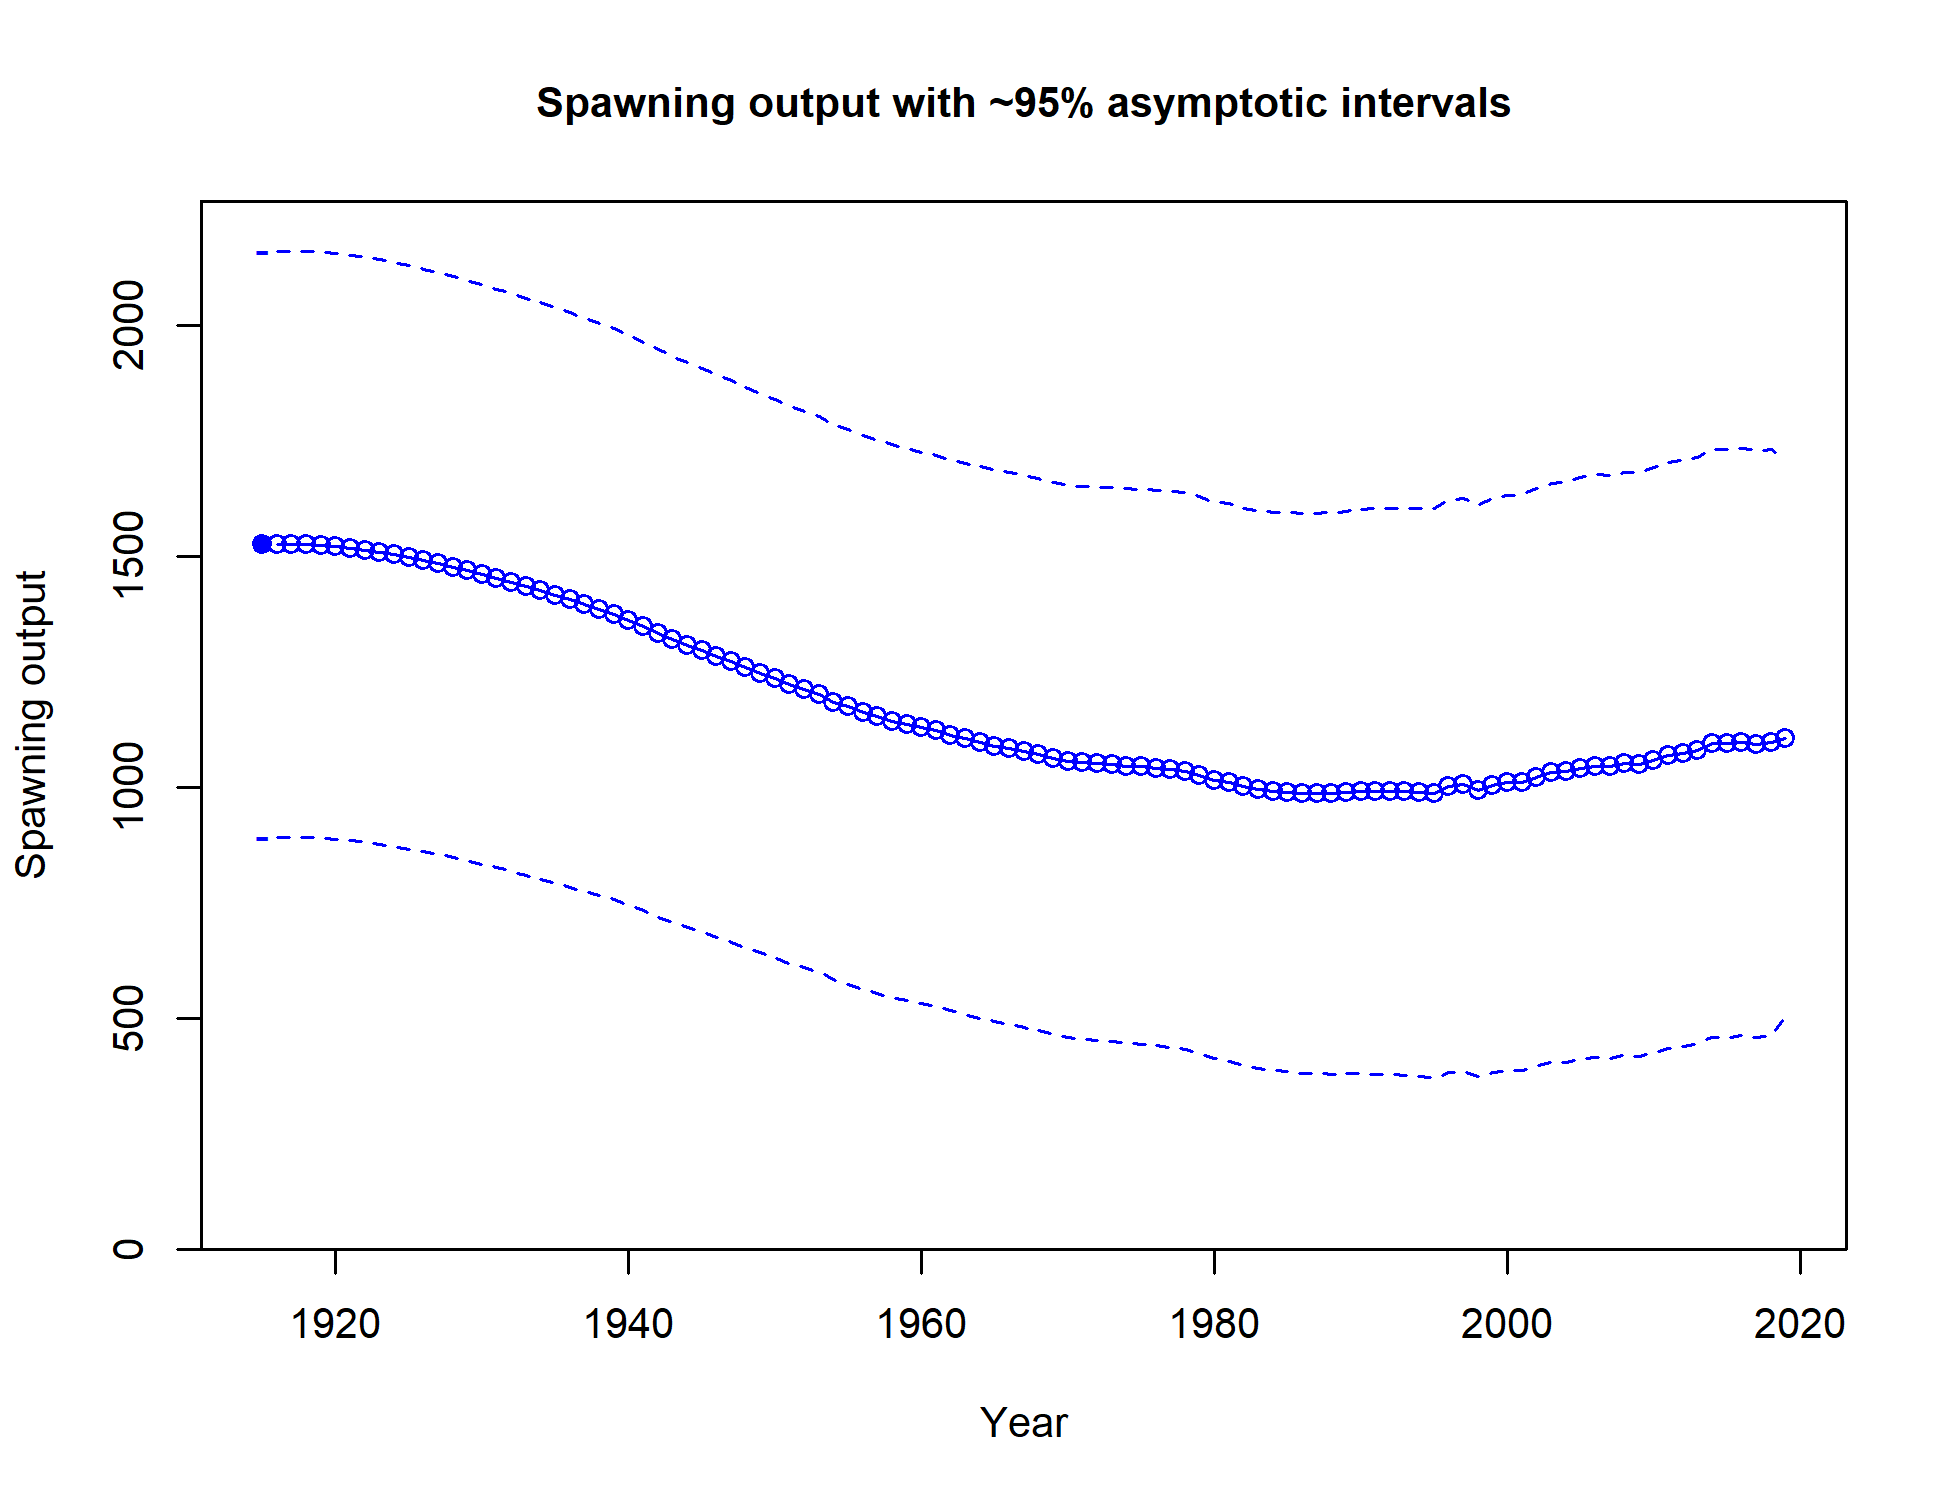
\includegraphics{r4ss/plots_mod1/ts7_Spawning_output_with_95_asymptotic_intervals_intervals.png}
\caption{Estimated spawning biomass (mt) with approximate 95\%
asymptotic intervals.
\label{fig:ts7_Spawning_biomass_(mt)_with_95_asymptotic_intervals_intervals}}
\end{figure}

\begin{figure}
\centering
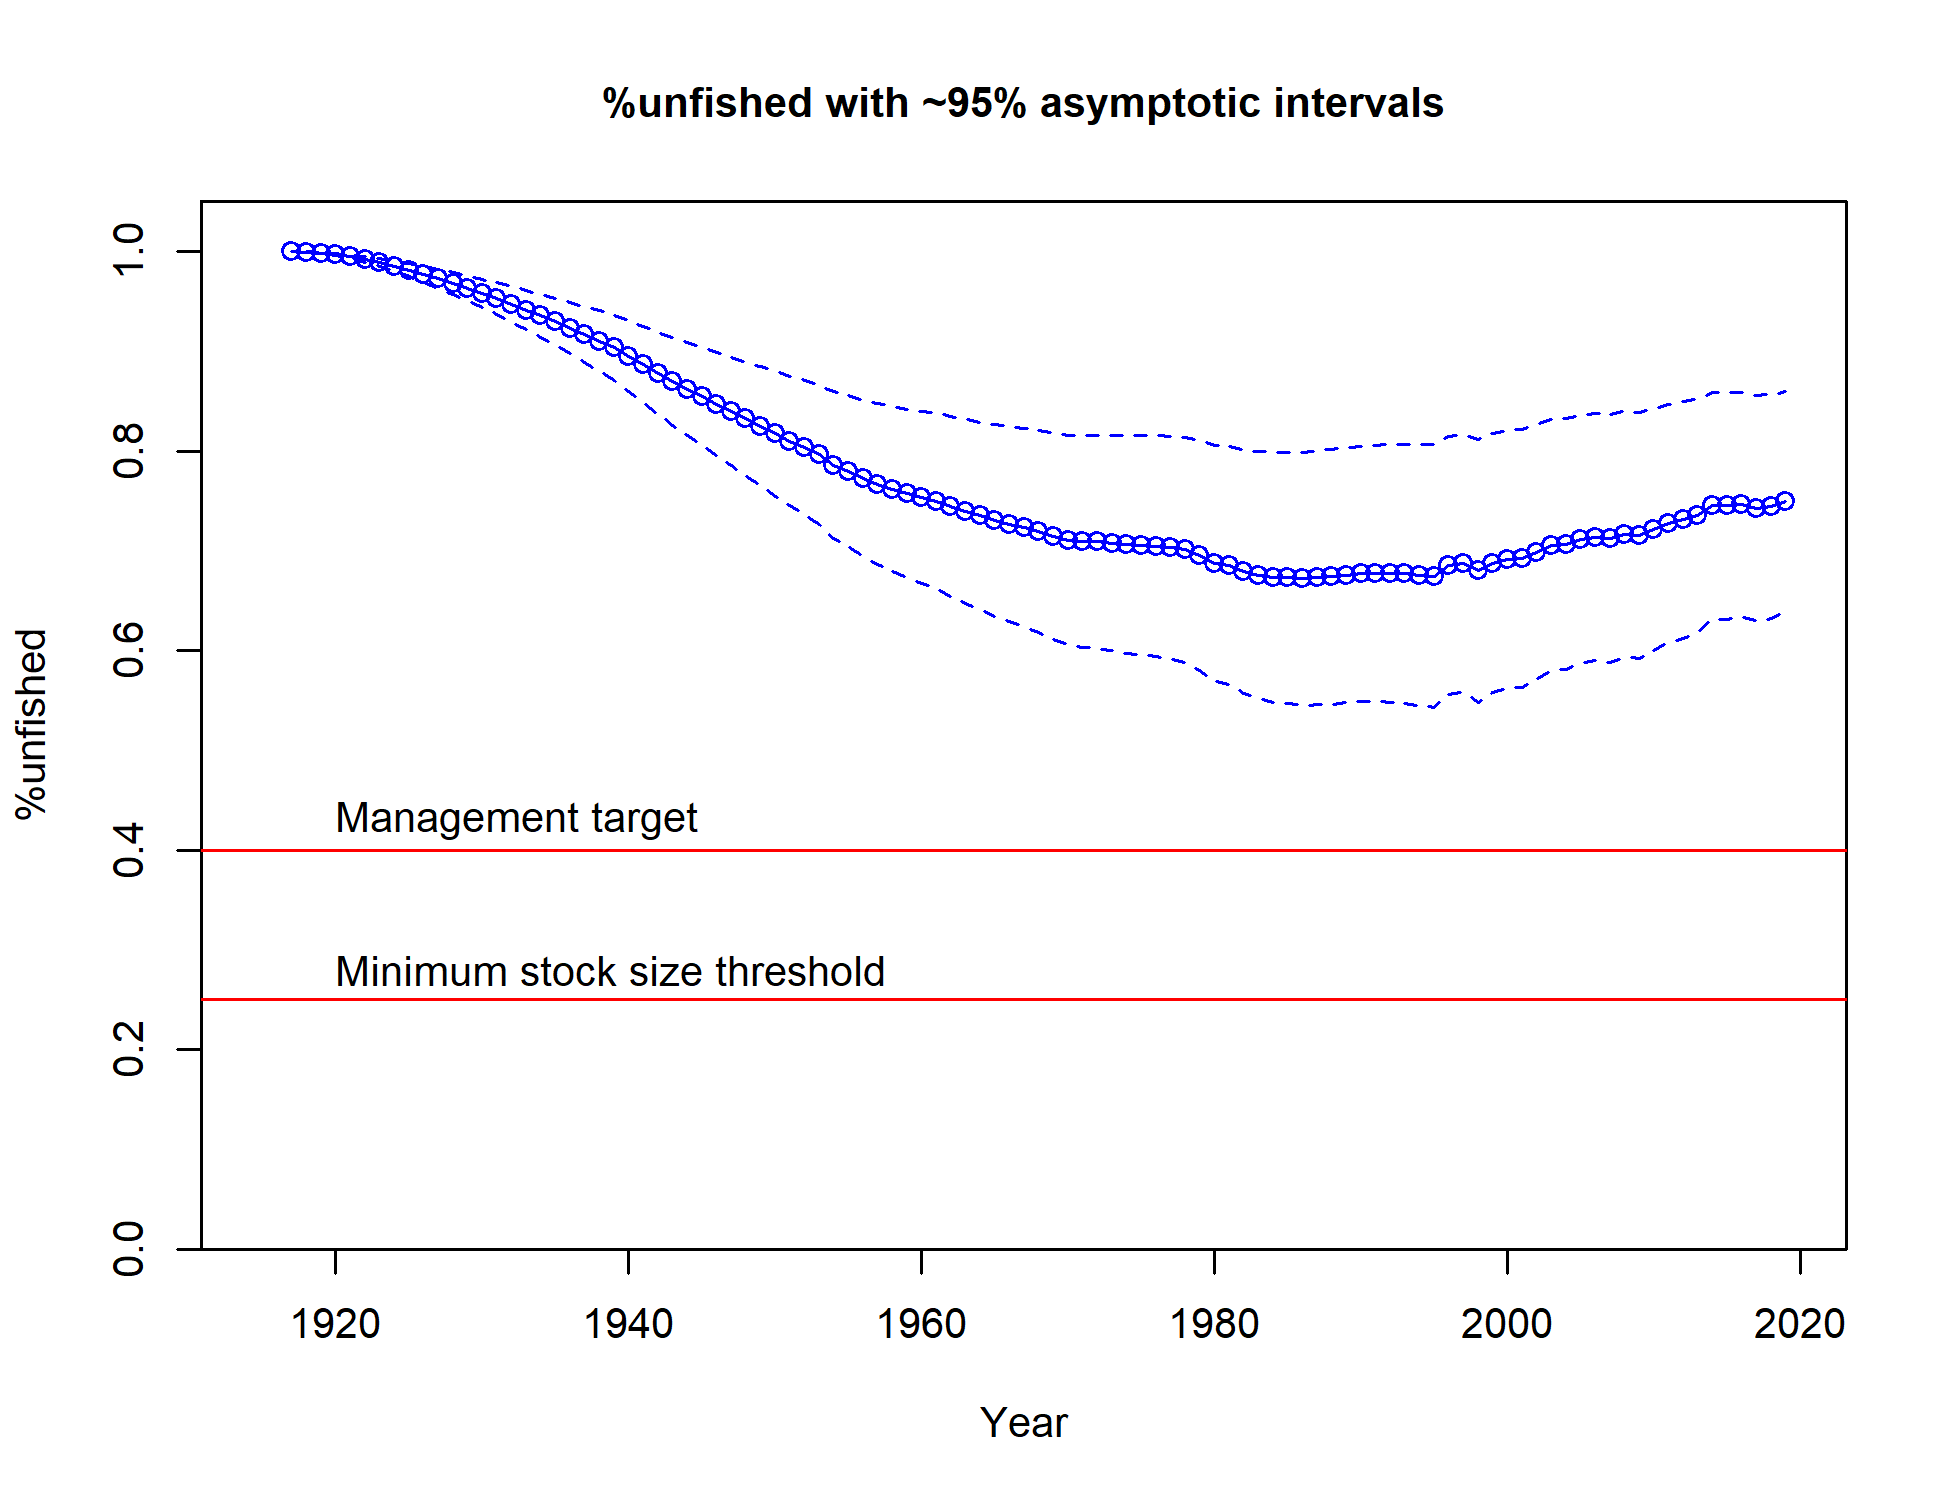
\includegraphics{r4ss/plots_mod1/ts9_Spawning_depletion_with_95_asymptotic_intervals_intervals.png}
\caption{Estimated spawning depletion with approximate 95\% asymptotic
intervals.
\label{fig:ts9_Spawning_depletion_with_95_asymptotic_intervals_intervals}}
\end{figure}

\begin{figure}
\centering
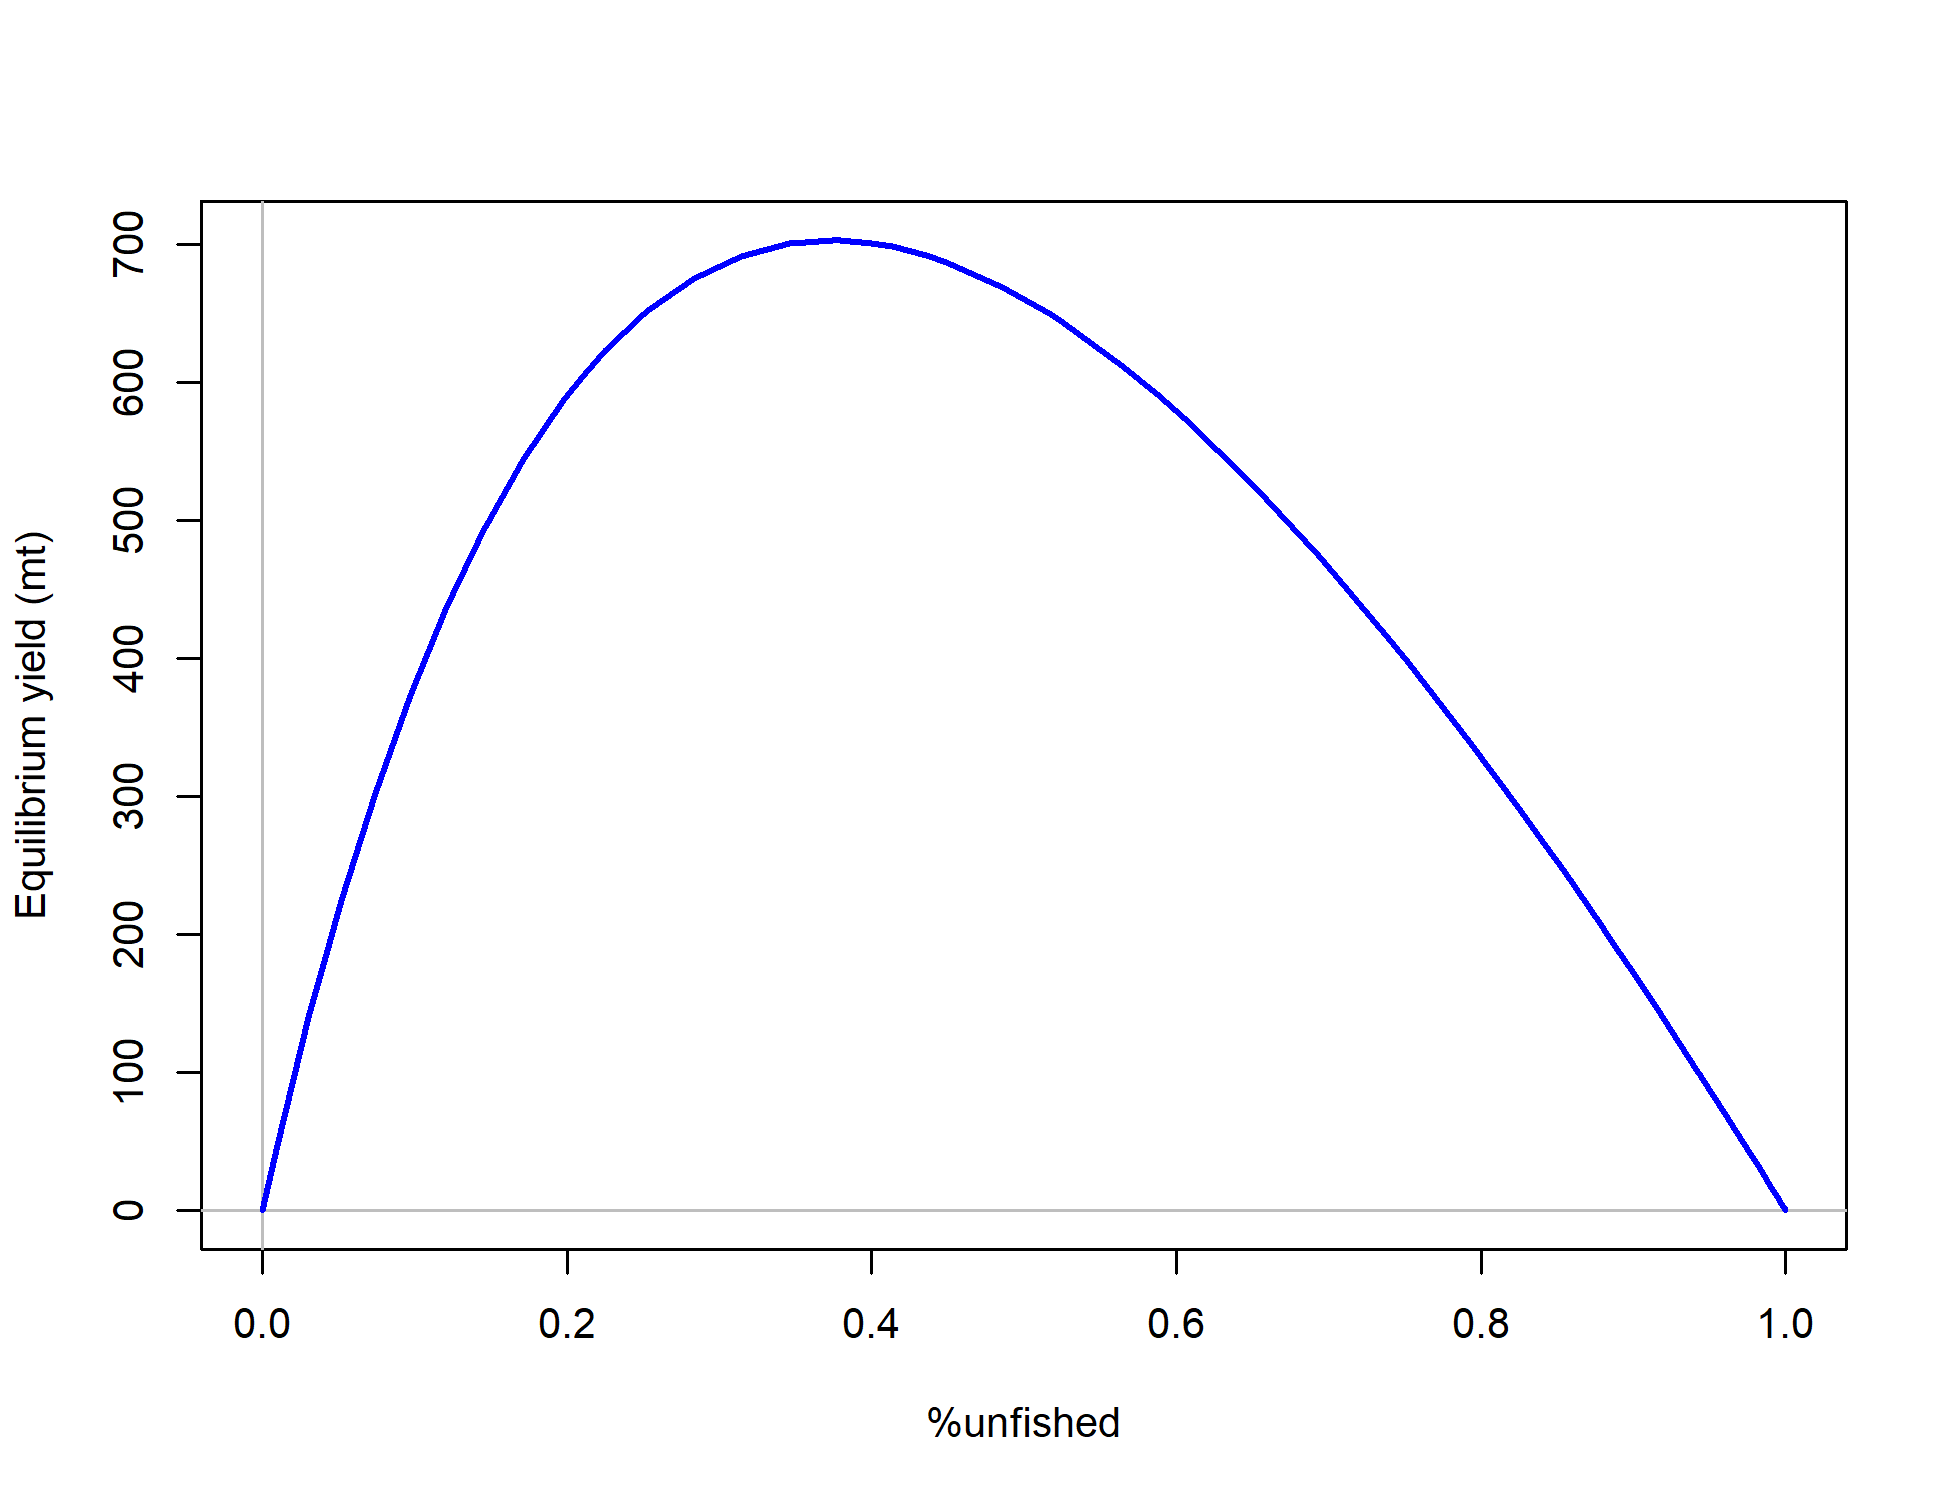
\includegraphics{r4ss/plots_mod1/yield1_yield_curve.png}
\caption{Equilibrium yield curve for the base case model. Values are
based on the 2018 fishery selectivity and with steepness fixed at 0.718.
\label{fig:yield1_yield_curve}}
\end{figure}

\FloatBarrier

\newpage

\FloatBarrier
\newpage

\#Appendix A. Detailed fits to length composition data \{-\}
\renewcommand{\thepage}{A-\arabic{page}}

\renewcommand{\thefigure}{A\arabic{figure}}
\setcounter{page}{1}

\begin{figure}
\centering
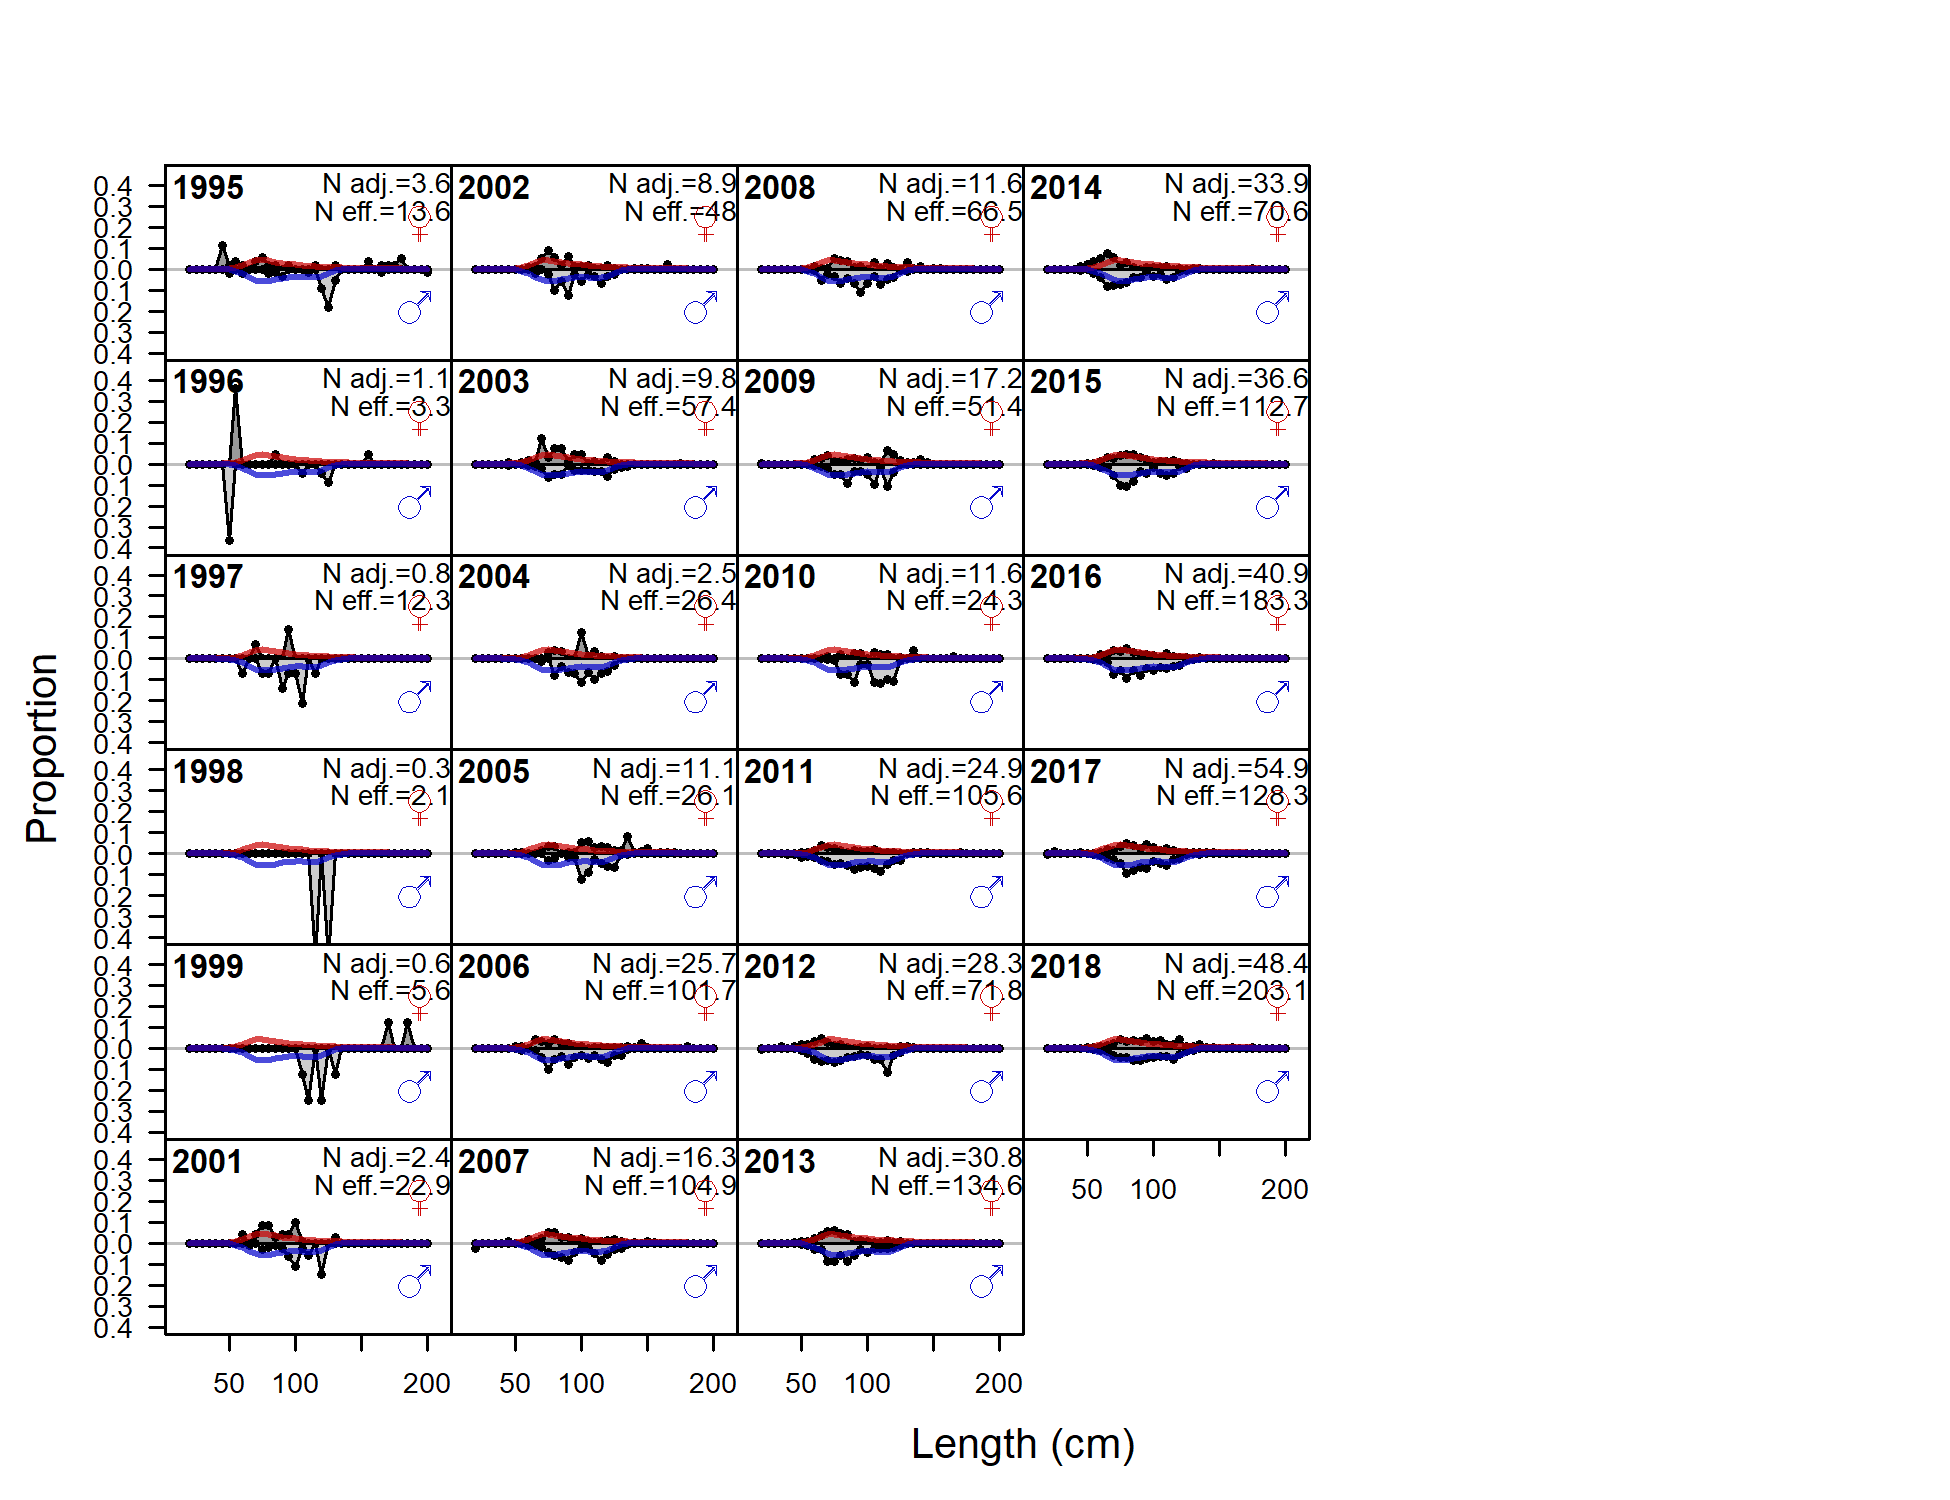
\includegraphics{./r4ss/plots_mod1/comp_lenfit_flt1mkt2.png}
\caption{Length comps, retained, Fishery\_current. `N adj.' is the input
sample size after data\_weighting adjustment. N eff. is the calculated
effective sample size used in the McAllister\_Iannelli tuning method.
\label{fig:mod1_1_comp_lenfit_flt1mkt2}}
\end{figure}

\begin{figure}
\centering
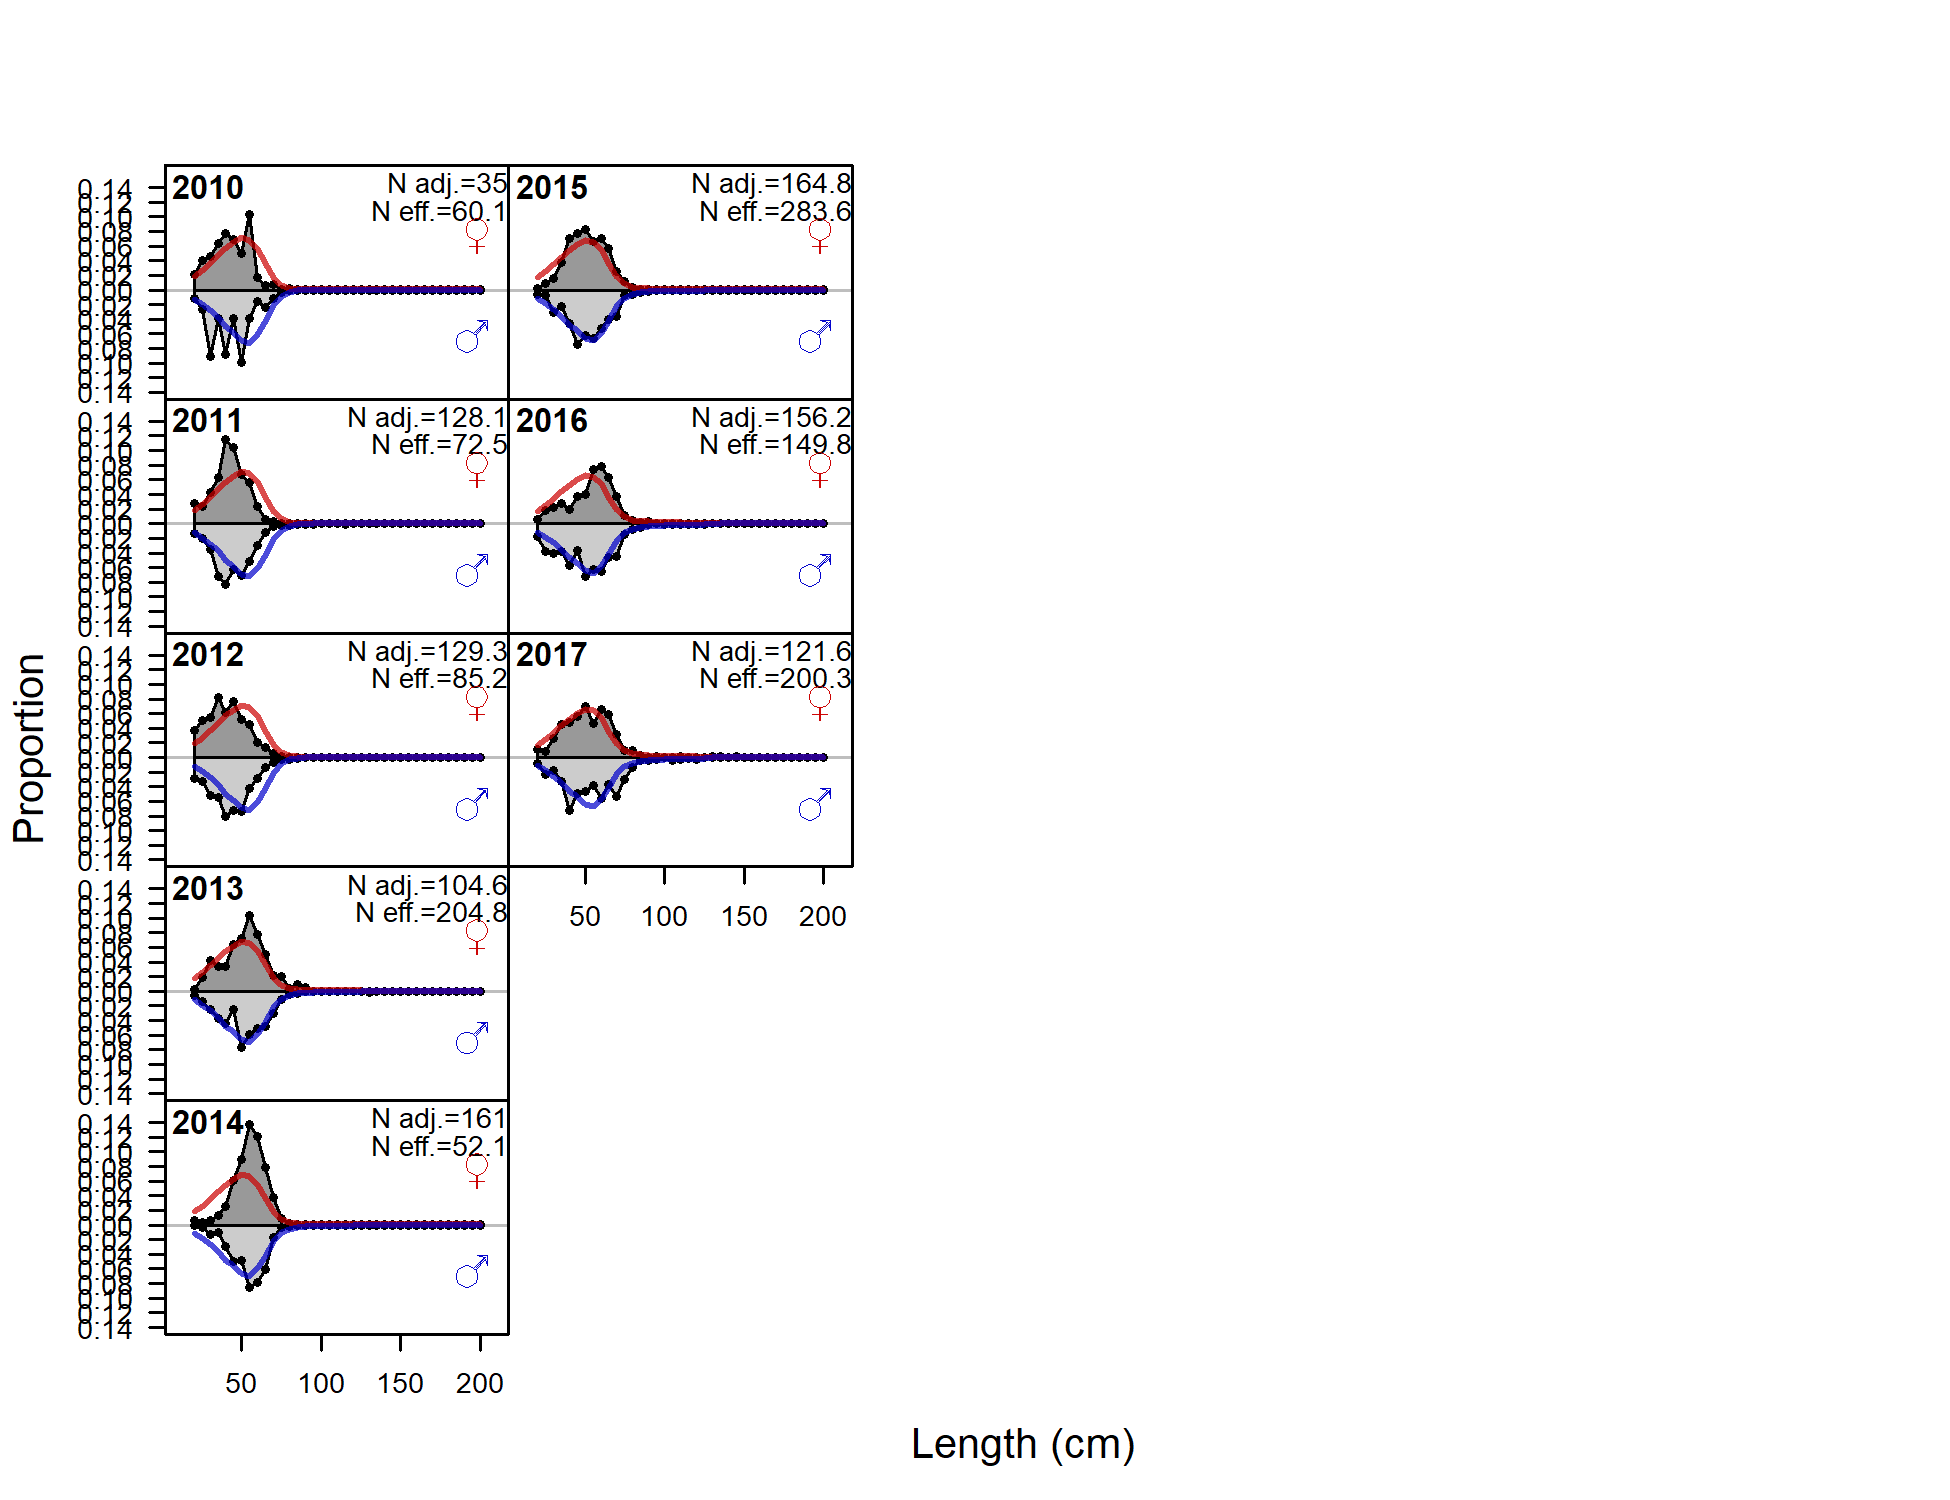
\includegraphics{./r4ss/plots_mod1/comp_lenfit_flt1mkt1.png}
\caption{Length comps, discard, Fishery\_current. `N adj.' is the input
sample size after data\_weighting adjustment. N eff. is the calculated
effective sample size used in the McAllister\_Iannelli tuning method.
\label{fig:mod1_2_comp_lenfit_flt1mkt1}}
\end{figure}

\begin{figure}
\centering
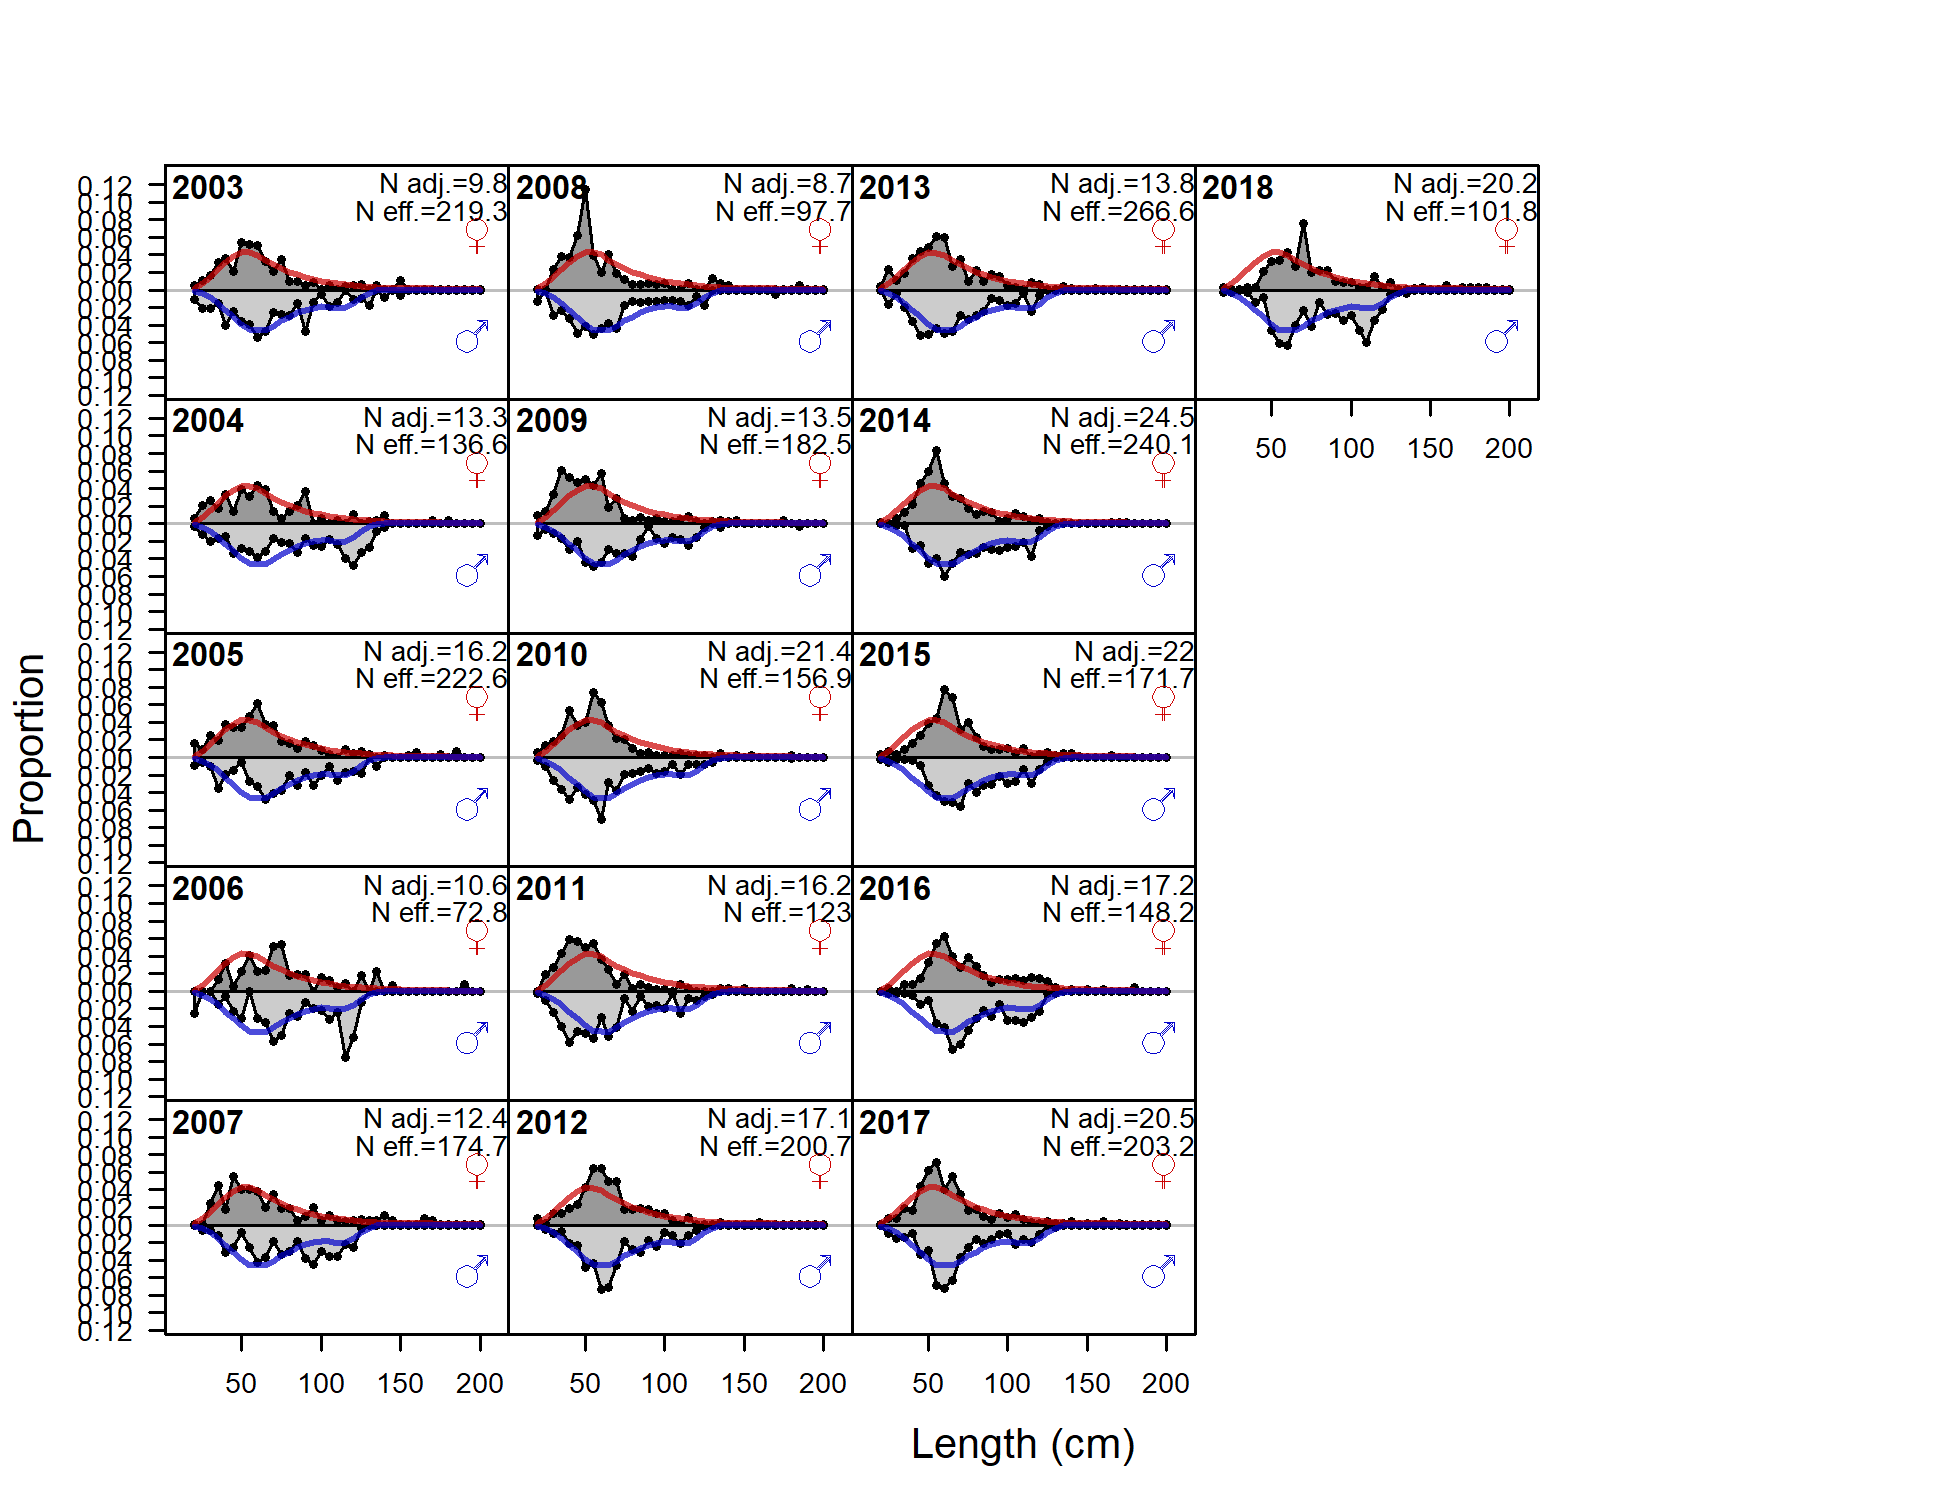
\includegraphics{./r4ss/plots_mod1/comp_lenfit_flt5mkt0.png}
\caption{Length comps, whole catch, WCGBTS. `N adj.' is the input sample
size after data\_weighting adjustment. N eff. is the calculated
effective sample size used in the McAllister\_Iannelli tuning method.
\label{fig:mod1_3_comp_lenfit_flt5mkt0}}
\end{figure}

\begin{figure}
\centering
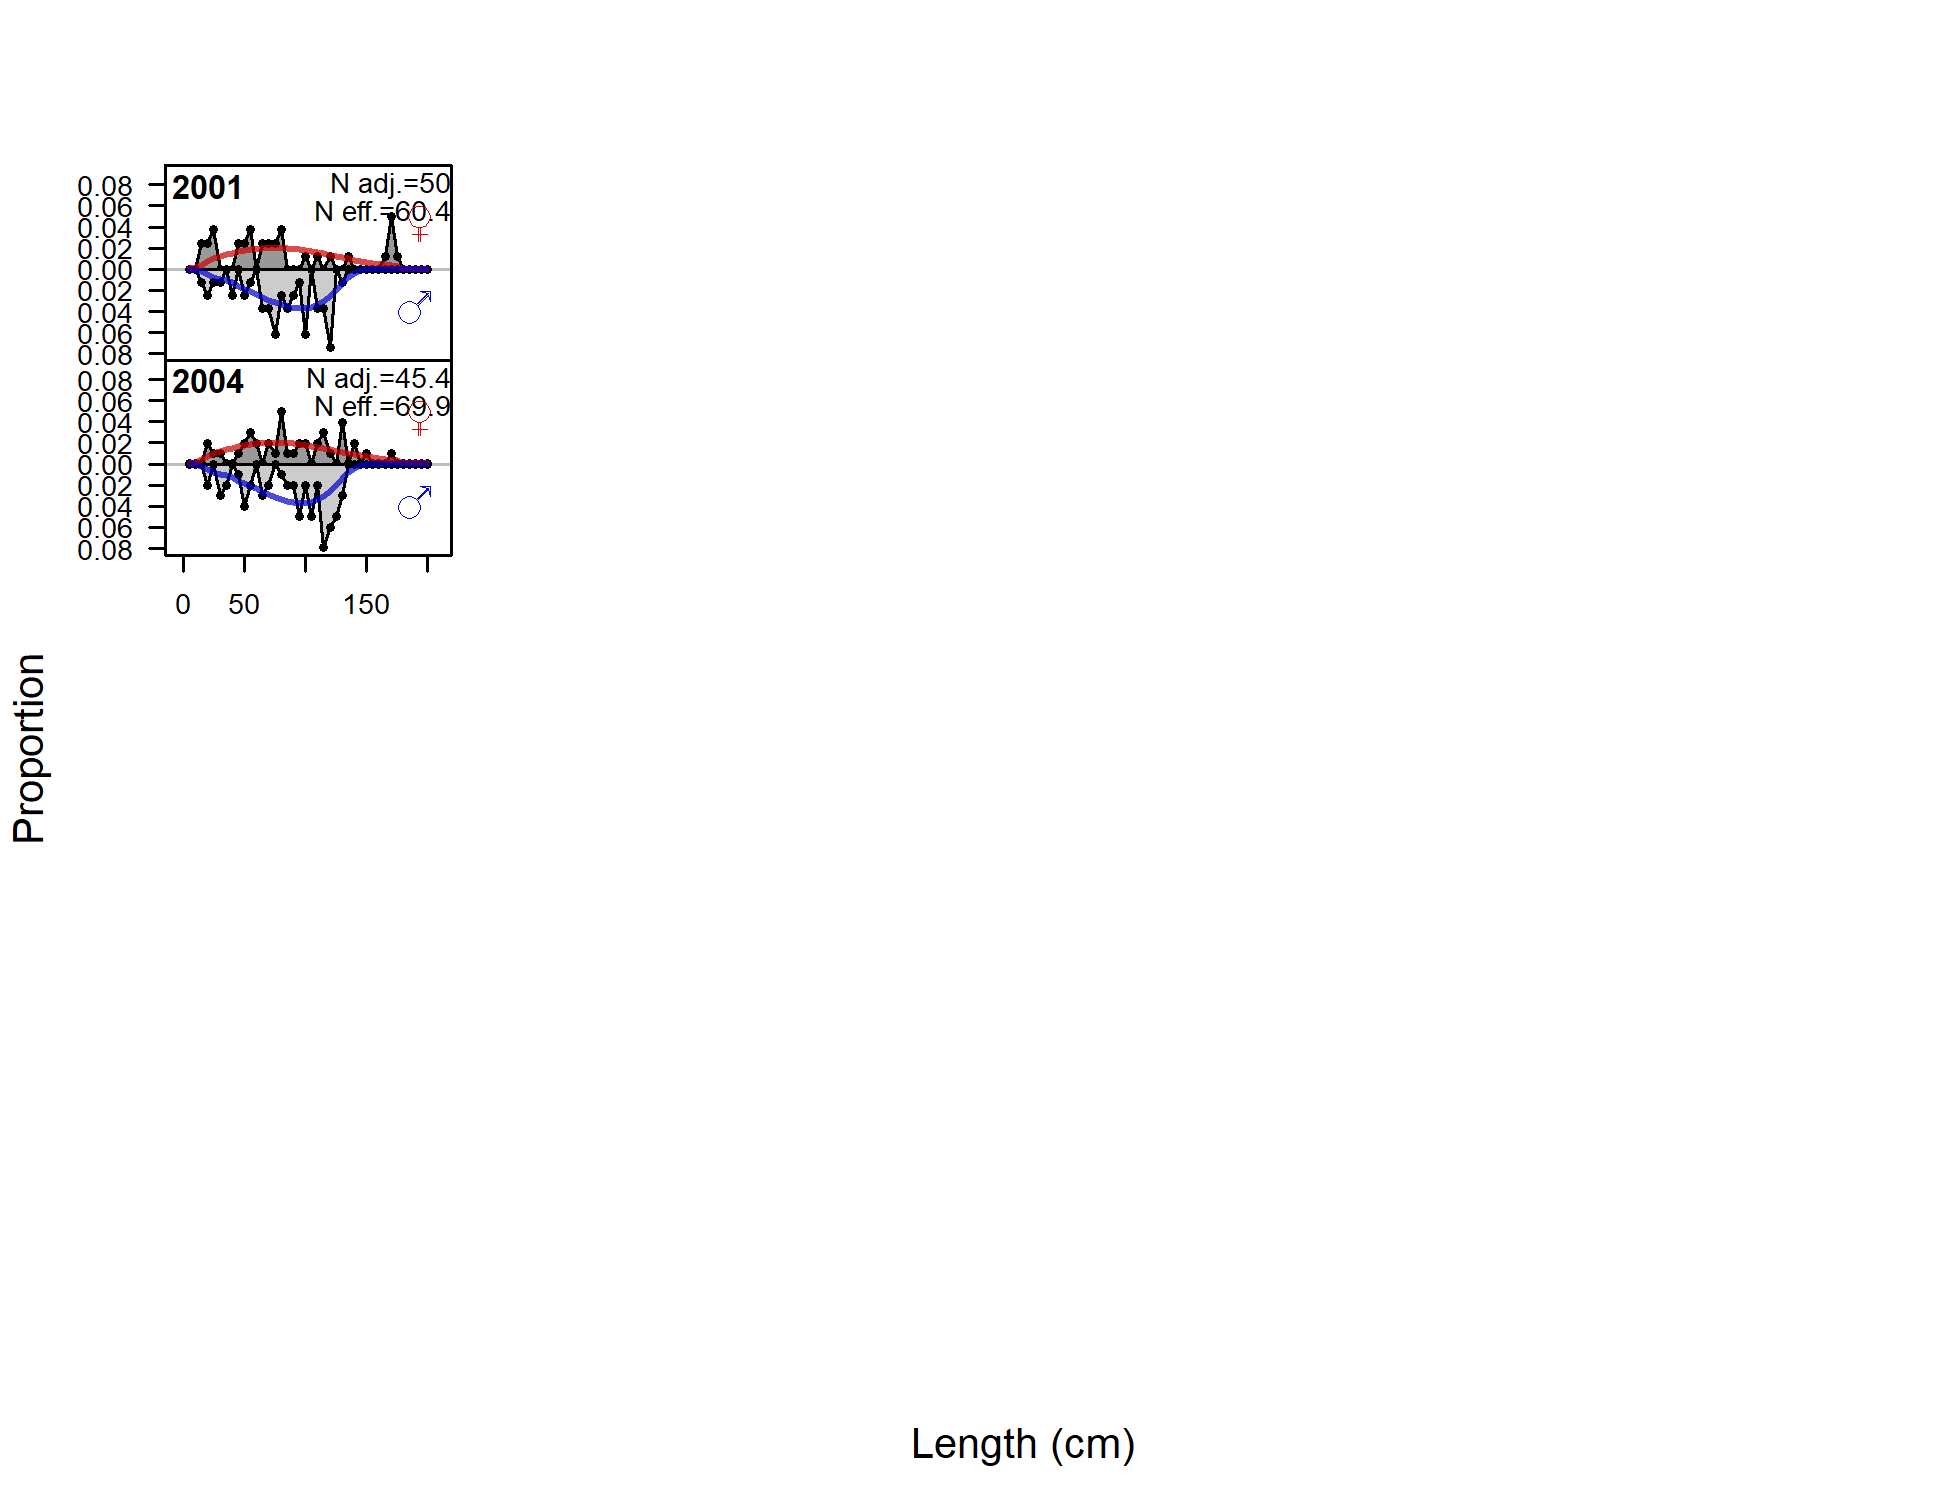
\includegraphics{./r4ss/plots_mod1/comp_lenfit_flt6mkt0.png}
\caption{Length comps, whole catch, Triennial. `N adj.' is the input
sample size after data\_weighting adjustment. N eff. is the calculated
effective sample size used in the McAllister\_Iannelli tuning method.
\label{fig:mod1_4_comp_lenfit_flt6mkt0}}
\end{figure}

\begin{figure}
\centering
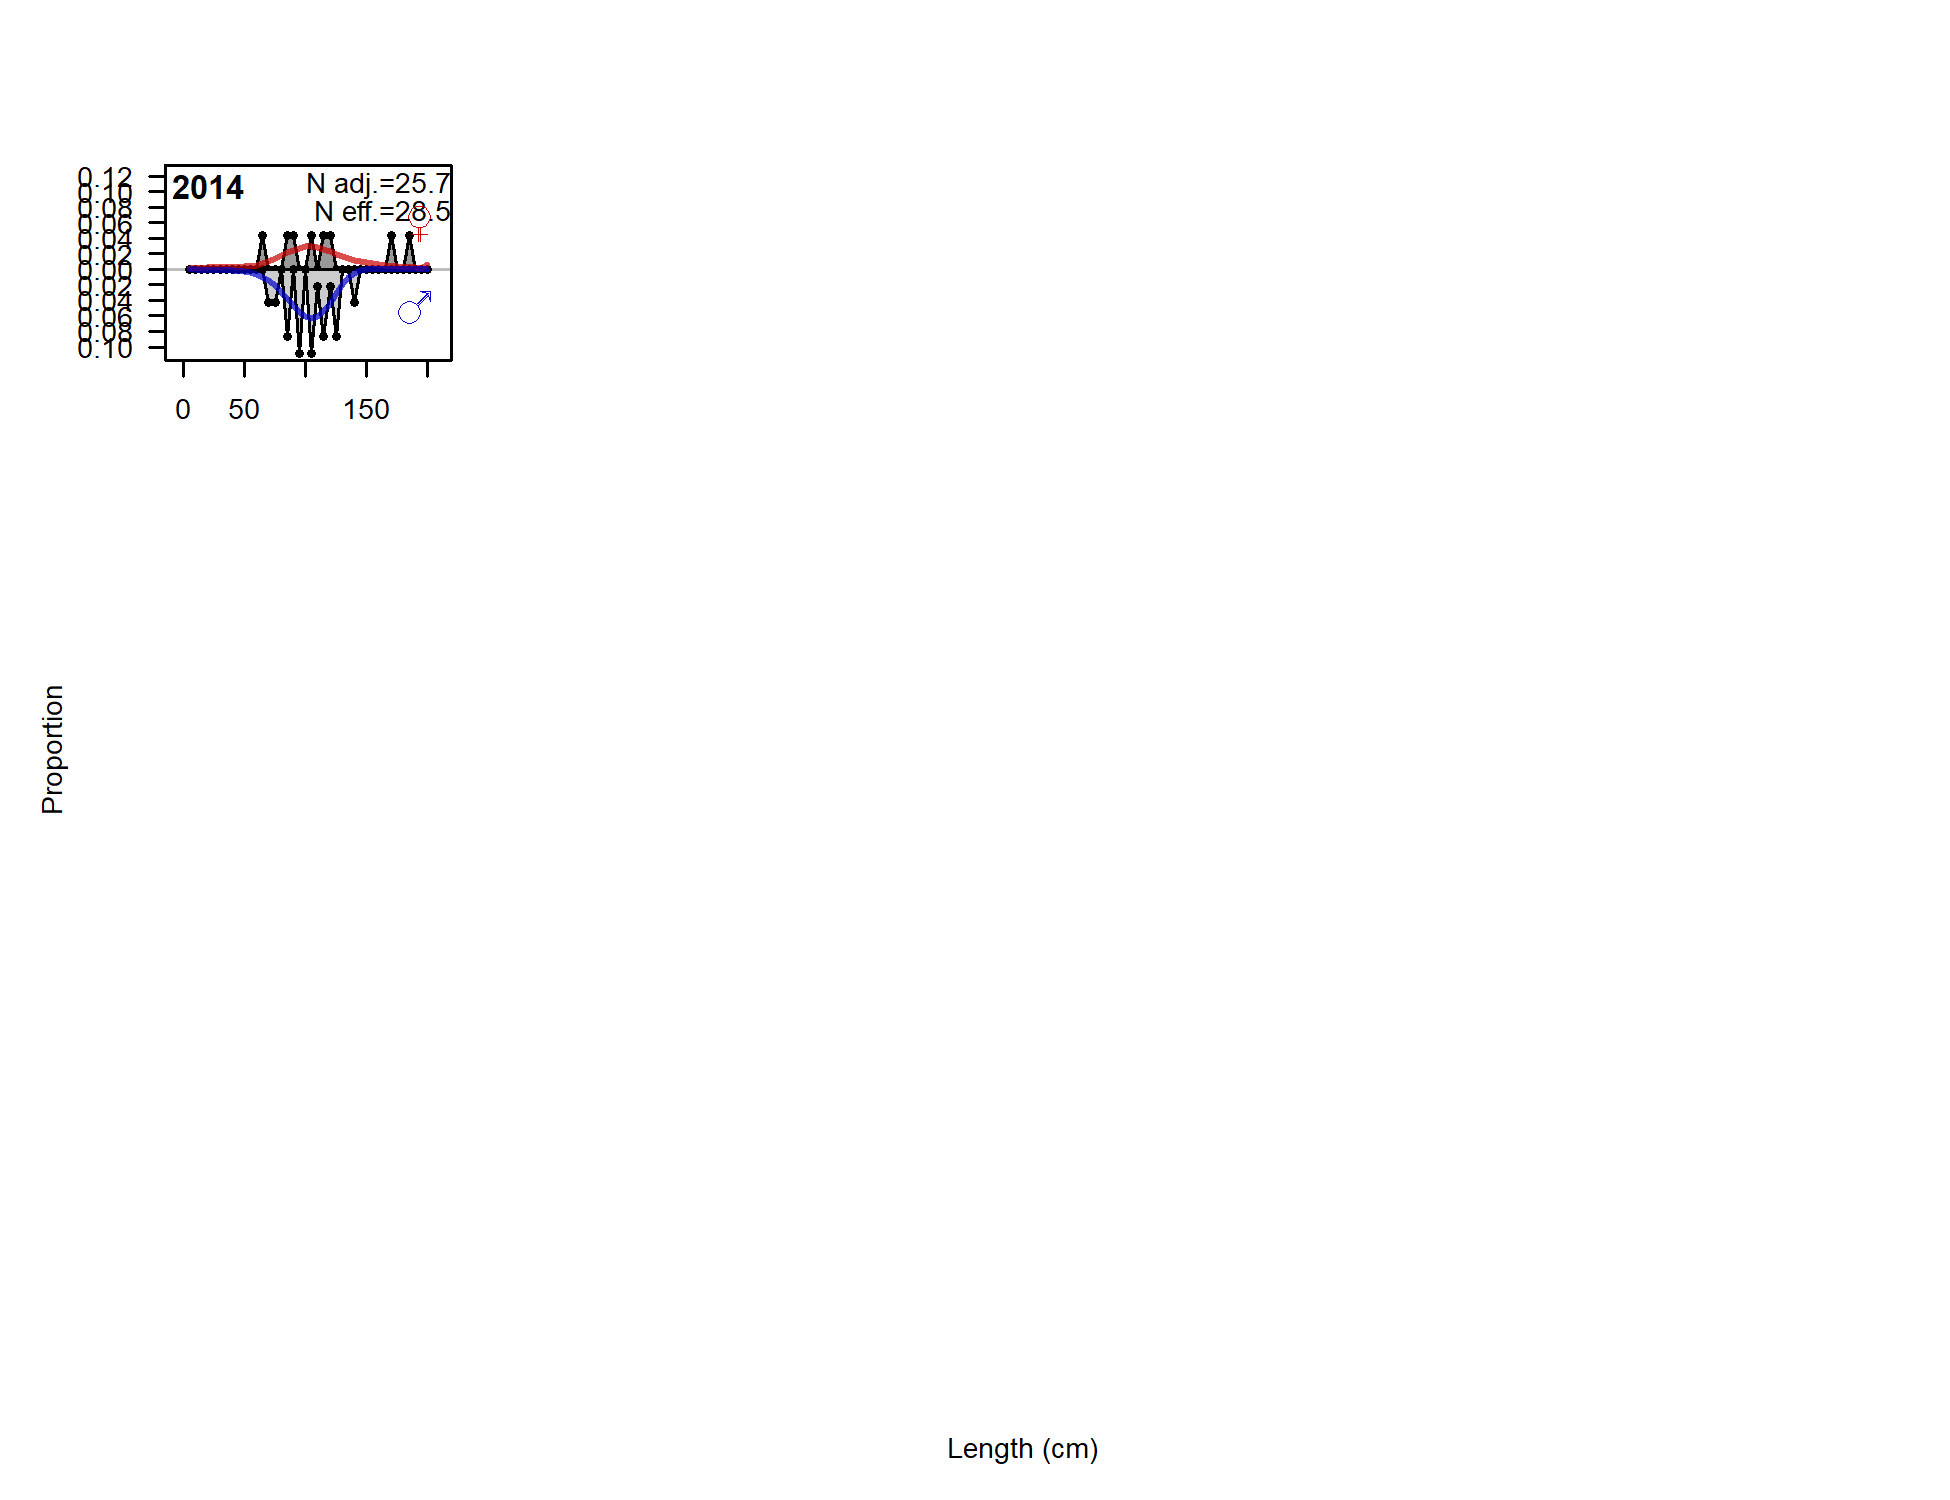
\includegraphics{./r4ss/plots_mod1/comp_lenfit_flt7mkt2.png}
\caption{Length comps, retained, IPHC. `N adj.' is the input sample size
after data\_weighting adjustment. N eff. is the calculated effective
sample size used in the McAllister\_Iannelli tuning method.
\label{fig:mod1_5_comp_lenfit_flt7mkt2}}
\end{figure}

\color{black}

\#References\{-\}

\renewcommand{\thepage}{}

\hypertarget{refs}{}
\leavevmode\hypertarget{ref-Bradburn2011}{}%
Bradburn, M.J. and Keller, A.A and Horness, B.H. (n.d.). The 2003 to
2008 US West Coast bottom trawl surveys of groundfish resources off
Washington, Oregon, and California: estimates of distribution,
abundance, length, and age composition. NOAA Technical Memorandum NMFS
NOAA-TM-NMFS-NWFSC-114: 323 pp.

\leavevmode\hypertarget{ref-Gunderson1980}{}%
Gunderson, Donald Raymond and Sample, Terrance M. (n.d.). Distribution
and abundance of rockfish off Washington, Oregon and California during
1977. Northwest and Alaska Fisheries Center, National Marine Fisheries
Service. Available from
\href{\%7Bhttp://spo.nmfs.noaa.gov/mfr423-4/mfr423-42.pdf\%7D}{\{http://spo.nmfs.noaa.gov/mfr423-4/mfr423-42.pdf\}}.

\leavevmode\hypertarget{ref-Hamel2015}{}%
Hamel, Owen S. (n.d.). A method for calculating a meta-analytical prior
for the natural mortality rate using multiple life history correlates.
ICES Journal of Marine Science: Journal du Conseil \textbf{72}(1):
62--69. doi:
\href{https://doi.org/\%7B10.1093/icesjms/fsu131\%7D}{\{10.1093/icesjms/fsu131\}}.

\leavevmode\hypertarget{ref-Keller2017}{}%
Keller, A.A. and Wallace, J.R. and Methot, R.D. (n.d.). The Northwest
Fisheries Science Center's West Coast Groundfish Bottom Trawl Survey:
History, Design, and Description. NOAA Technical Memorandum NMFS
NOAA-TM-NMFS-NWFSC-136: 38 pp.

\leavevmode\hypertarget{ref-Love1987}{}%
Love, Milton S and Axell, Brita and Morris, Pamela and Collins, Robson
and Brooks, Andrew. (n.d.). Life history and fishery of the California
scorpionfish,\\
emphScorpaena guttata, within the Southern California Bight. Fishery
Bulletin \textbf{85}: 99--116.

\leavevmode\hypertarget{ref-Thorson2015}{}%
Thorson, J. T. and Shelton, A. O. and Ward, E. J. and Skaug, H. J.
(n.d.). Geostatistical delta-generalized linear mixed models improve
precision for estimated abundance indices for West Coast groundfishes.
ICES Journal of Marine Science \textbf{72}(5): 1297--1310. doi:
\href{https://doi.org/\%7B10.1093/icesjms/fsu243\%7D}{\{10.1093/icesjms/fsu243\}}.

\end{document}
